%!TEX root = ../main.tex
\chapter{Termodinamica}

\section{Introduzione generale}

\paragraph{Esempio} Secondo il teorema dell'energia meccanica essa varia se agiscono forze non conservative che compiono lavoro. Ci sono casi in cui l'energia meccanica si dissipa, per esempio a causa dell'effetto della forza d'attrito. Si consideri la situazione in cui un corpo è fermo in cima ad un piano liscio inclinato che termina con un piano orizzontale scabro. Quando esso viene lasciato libero di scivolare, la sua energia potenziale si trasforma in energia cinetica che lo fa scendere verso il basso. Poi il corpo striscia sul piano con attrito fino a fermarsi, arrivando ad avere energia cinetica nulla. Se si ripete tante volte l'esperimento, si sente che il tavolo si è scaldato. Si comincia a capire che l'energia non è svanita ma si è trasformata in un altra forma. L'effetto dello strisciamento fa si che le molecole del piano si mettano a vibrare dando luogo a un moto di agitazione termica. Il moto ordinato si trasforma in un moto disordinato delle molecole che stanno sulla superficie del tavolo e vengono agitate.
Tramite gli urti fra il reticolo cristallino del materiale e il piano scabro, l'energia cinetica si è trasformata in calore. Quindi, il lavoro fatto da un corpo si può trasformare in calore ceduto.

Uno degli argomenti principali della termodinamica quindi è proprio l'esame del bilancio energetico complessivo di un processo fisico, esteso a scambi di energia che non sono meccanici nel senso macroscopico finora descritto.
Storicamente la termodinamica nasce con una valenza concreta, che è quella di riuscire a realizzare delle macchine che invertano questo processo descritto nell'esempio. Le \textbf{macchine termiche} (un esempio ne è quella a vapore) sono proprio dei dispositivi che sfruttando il calore ceduto da un corpo caldo, riuscendo a trasformarne una parte in lavoro meccanico. Non è infatti possibile trasformare tutto il calore disponibile, perché c'è sempre una parte di energia che diventa termica. Altro obiettivo della termodinamica è quello in realizzare \textbf{macchine frigorifere}, dispositivi che permettono il passaggio di calore da un corpo più freddo a un corpo più caldo.
In termodinamica non si mantiene lo stesso approccio microscopico utilizzato per lo studio della meccanica. Si immagini di avere un certo gas in una stanza. Esso è chiuso da un coperchio che si può muovere, sopra il quale è posta una massa $m$. Si vuole realizzare un processo per sollevarla. Si può fare ciò mettendo il contenitore su un fornello che cede il calore al gas: esso scaldandosi tende a espandersi e arriva a sollevare il pistone.

\begin{figure}[htpb]
	\centering

	% Pattern Info
	 
	\tikzset{
	pattern size/.store in=\mcSize, 
	pattern size = 5pt,
	pattern thickness/.store in=\mcThickness, 
	pattern thickness = 0.3pt,
	pattern radius/.store in=\mcRadius, 
	pattern radius = 1pt}
	\makeatletter
	\pgfutil@ifundefined{pgf@pattern@name@_w62qczmze}{
	\pgfdeclarepatternformonly[\mcThickness,\mcSize]{_w62qczmze}
	{\pgfqpoint{0pt}{0pt}}
	{\pgfpoint{\mcSize}{\mcSize}}
	{\pgfpoint{\mcSize}{\mcSize}}
	{
	\pgfsetcolor{\tikz@pattern@color}
	\pgfsetlinewidth{\mcThickness}
	\pgfpathmoveto{\pgfqpoint{0pt}{\mcSize}}
	\pgfpathlineto{\pgfpoint{\mcSize+\mcThickness}{-\mcThickness}}
	\pgfpathmoveto{\pgfqpoint{0pt}{0pt}}
	\pgfpathlineto{\pgfpoint{\mcSize+\mcThickness}{\mcSize+\mcThickness}}
	\pgfusepath{stroke}
	}}
	\makeatother
	\tikzset{every picture/.style={line width=0.75pt}} %set default line width to 0.75pt        

	\begin{tikzpicture}[x=0.75pt,y=0.75pt,yscale=-1,xscale=1]
	%uncomment if require: \path (0,300); %set diagram left start at 0, and has height of 300

	%Shape: Rectangle [id:dp8385749660235218] 
	\draw  [fill={rgb, 255:red, 155; green, 155; blue, 155 }  ,fill opacity=1 ] (183,99) -- (213,99) -- (213,119) -- (183,119) -- cycle ;
	%Straight Lines [id:da657731717925097] 
	\draw    (150,112) -- (150,220) ;
	%Straight Lines [id:da7283267698919824] 
	\draw    (240,112) -- (240,220) ;
	%Straight Lines [id:da4943759947161752] 
	\draw    (150,220) -- (240,220) ;
	%Straight Lines [id:da3363410918516512] 
	\draw [line width=2.25]    (150,120) -- (240,120) ;
	%Shape: Circle [id:dp1531034878009534] 
	\draw  [draw opacity=0][fill={rgb, 255:red, 212; green, 212; blue, 212 }  ,fill opacity=1 ] (159,139.13) .. controls (159,134.64) and (162.64,131) .. (167.13,131) .. controls (171.61,131) and (175.25,134.64) .. (175.25,139.13) .. controls (175.25,143.61) and (171.61,147.25) .. (167.13,147.25) .. controls (162.64,147.25) and (159,143.61) .. (159,139.13) -- cycle ;
	%Shape: Circle [id:dp16555656889441606] 
	\draw  [draw opacity=0][fill={rgb, 255:red, 212; green, 212; blue, 212 }  ,fill opacity=1 ] (185.5,140.63) .. controls (185.5,136.14) and (189.14,132.5) .. (193.63,132.5) .. controls (198.11,132.5) and (201.75,136.14) .. (201.75,140.63) .. controls (201.75,145.11) and (198.11,148.75) .. (193.63,148.75) .. controls (189.14,148.75) and (185.5,145.11) .. (185.5,140.63) -- cycle ;
	%Shape: Circle [id:dp2325841443862715] 
	\draw  [draw opacity=0][fill={rgb, 255:red, 212; green, 212; blue, 212 }  ,fill opacity=1 ] (206,156.13) .. controls (206,151.64) and (209.64,148) .. (214.13,148) .. controls (218.61,148) and (222.25,151.64) .. (222.25,156.13) .. controls (222.25,160.61) and (218.61,164.25) .. (214.13,164.25) .. controls (209.64,164.25) and (206,160.61) .. (206,156.13) -- cycle ;
	%Shape: Circle [id:dp23279454300641023] 
	\draw  [draw opacity=0][fill={rgb, 255:red, 212; green, 212; blue, 212 }  ,fill opacity=1 ] (167.5,157.13) .. controls (167.5,152.64) and (171.14,149) .. (175.63,149) .. controls (180.11,149) and (183.75,152.64) .. (183.75,157.13) .. controls (183.75,161.61) and (180.11,165.25) .. (175.63,165.25) .. controls (171.14,165.25) and (167.5,161.61) .. (167.5,157.13) -- cycle ;
	%Shape: Circle [id:dp1344282787670925] 
	\draw  [draw opacity=0][fill={rgb, 255:red, 212; green, 212; blue, 212 }  ,fill opacity=1 ] (185,169.63) .. controls (185,165.14) and (188.64,161.5) .. (193.13,161.5) .. controls (197.61,161.5) and (201.25,165.14) .. (201.25,169.63) .. controls (201.25,174.11) and (197.61,177.75) .. (193.13,177.75) .. controls (188.64,177.75) and (185,174.11) .. (185,169.63) -- cycle ;
	%Shape: Circle [id:dp3125843154048371] 
	\draw  [draw opacity=0][fill={rgb, 255:red, 212; green, 212; blue, 212 }  ,fill opacity=1 ] (161,180.63) .. controls (161,176.14) and (164.64,172.5) .. (169.13,172.5) .. controls (173.61,172.5) and (177.25,176.14) .. (177.25,180.63) .. controls (177.25,185.11) and (173.61,188.75) .. (169.13,188.75) .. controls (164.64,188.75) and (161,185.11) .. (161,180.63) -- cycle ;
	%Shape: Circle [id:dp2629546156324918] 
	\draw  [draw opacity=0][fill={rgb, 255:red, 212; green, 212; blue, 212 }  ,fill opacity=1 ] (212,179.63) .. controls (212,175.14) and (215.64,171.5) .. (220.13,171.5) .. controls (224.61,171.5) and (228.25,175.14) .. (228.25,179.63) .. controls (228.25,184.11) and (224.61,187.75) .. (220.13,187.75) .. controls (215.64,187.75) and (212,184.11) .. (212,179.63) -- cycle ;
	%Shape: Circle [id:dp8643090492517644] 
	\draw  [draw opacity=0][fill={rgb, 255:red, 212; green, 212; blue, 212 }  ,fill opacity=1 ] (191.5,190.63) .. controls (191.5,186.14) and (195.14,182.5) .. (199.63,182.5) .. controls (204.11,182.5) and (207.75,186.14) .. (207.75,190.63) .. controls (207.75,195.11) and (204.11,198.75) .. (199.63,198.75) .. controls (195.14,198.75) and (191.5,195.11) .. (191.5,190.63) -- cycle ;
	%Shape: Circle [id:dp9763411767245602] 
	\draw  [draw opacity=0][fill={rgb, 255:red, 212; green, 212; blue, 212 }  ,fill opacity=1 ] (211,205.13) .. controls (211,200.64) and (214.64,197) .. (219.13,197) .. controls (223.61,197) and (227.25,200.64) .. (227.25,205.13) .. controls (227.25,209.61) and (223.61,213.25) .. (219.13,213.25) .. controls (214.64,213.25) and (211,209.61) .. (211,205.13) -- cycle ;
	%Shape: Circle [id:dp04886257473073541] 
	\draw  [draw opacity=0][fill={rgb, 255:red, 212; green, 212; blue, 212 }  ,fill opacity=1 ] (172,204.63) .. controls (172,200.14) and (175.64,196.5) .. (180.13,196.5) .. controls (184.61,196.5) and (188.25,200.14) .. (188.25,204.63) .. controls (188.25,209.11) and (184.61,212.75) .. (180.13,212.75) .. controls (175.64,212.75) and (172,209.11) .. (172,204.63) -- cycle ;
	%Shape: Trapezoid [id:dp5293639465287374] 
	\draw  [pattern=_w62qczmze,pattern size=3pt,pattern thickness=0.75pt,pattern radius=0pt, pattern color={rgb, 255:red, 222; green, 222; blue, 222}] (161.5,220) -- (165.93,234.75) -- (224.08,234.75) -- (228.5,220) -- cycle ;
	%Shape: Circle [id:dp9592351510731913] 
	\draw  [draw opacity=0][fill={rgb, 255:red, 212; green, 212; blue, 212 }  ,fill opacity=1 ] (216,136.13) .. controls (216,131.64) and (219.64,128) .. (224.13,128) .. controls (228.61,128) and (232.25,131.64) .. (232.25,136.13) .. controls (232.25,140.61) and (228.61,144.25) .. (224.13,144.25) .. controls (219.64,144.25) and (216,140.61) .. (216,136.13) -- cycle ;

	% Text Node
	\draw (197.5,106) node    {$m$};

	\end{tikzpicture}
\end{figure}
\FloatBarrier
Tramite energia termica si è compiuto lavoro meccanico. Per usare un approccio microscopico si dovrebbero considerare tutte le innumerevoli molecole del gas e vedere come si muovono sotto l'azione dell'energia termica, cosa ovviamente impossibile. Si vanno invece a definire delle \textbf{variabili termodinamiche}, che permettono di descrivere nel complesso quello che succede al gas, basandosi sul suo comportamento osservato da un punto di vista macroscopico. Il sapere come si muovono in moto disordinato, anche detto \emph{browniano}, le particelle del gas non è molto utile per capire come si muove il pistone verso l'alto. Insomma, non si studierà più il moto di punti materiali, ma i passaggi energetici da un corpo a un altro.

La definizione stessa di stato termodinamico è concettualmente diversa da quella di stato meccanico, per il quale, in linea di principio, si presuppone la conoscenza di posizione e velocità di ciascuno dei punti. In questi termini un sistema termodinamico non è definibile. In effetti, se è noto lo stato termodinamico, non lo è in generale quello meccanico, anzi, a un dato stato termodinamico possono corrispondere moltissimi stati meccanici diversi. La descrizione termodinamica di un sistema e dei suoi scambi energetici, tramite le variabili termodinamiche, porta a conclusioni di grande generalità, applicabili a sistemi molto diversi tra loro. Tale descrizione però non può fornire informazioni sulle caratteristiche microscopiche del sistema, che vanno studiate concettualmente in modo diverso.

\section{I sistemi termodinamici}

\subsection{Definizione e caratteristiche generali}

Un \textbf{sistema termodinamico} è una porzione di spazio materiale, separata dal resto dell'ambiente esterno mediante una superficie di controllo. La parte o l'insieme delle parti con cui il sistema può interagire, prende il nome di \textbf{ambiente termodinamico}. Esso, nel caso prima citato è costituito dal fornello, dalla massa sul pistone e dallo spazio attorno ad esso. L'insieme sistema più ambiente si chiama \textbf{universo termodinamico}. La superficie che separa sistema termodinamico può essere reale o immaginaria e, a seconda dei passaggi che essa permette, il sistema termodinamico può essere classificato in tre tipologie:

\begin{itemize}
	\item Aperto: il confine permette il passaggio sia di energia sia di materia.
	\item Chiuso: il confine permette scambi di energia ma non di materia.
	\item Isolato: nessuno scambio è permesso.
\end{itemize}

Come già anticipato, per descrivere macroscopicamente un sistema termodinamico si introducono delle variabili termodinamiche che vanno a descrivere lo stato del sistema. Esse sono la pressione, la temperatura, il volume e la quantità di materia presente, ossia il numero di moli $n$.
Le variabili termodinamiche si distinguono in:

\begin{itemize}
	\item Variabili \textbf{intensive} (o locali): sono funzione della posizione (come la pressione o la temperatura);
	\item Variabili \textbf{estensive} (o globali): danno un'informazione generale, appunto, globale sul sistema. Esse sono ad esempio il volume o la quantità di materia.
\end{itemize}

Quando il sistema termodinamico è in equilibrio, esistono delle relazioni matematiche tra le variabili termodinamiche che prendono il nome di \textbf{funzioni di stato}: esse sussistono \emph{solo nella situazione in cui il sistema è in equilibrio}.

\[
	f(p,T,V,n) = 0
\]

\paragraph{Esempio} Quando un gas ideale viene mantenuto a temperatura costante e si espande in volume, la pressione diminuisce. Se la temperatura è costante, anche il prodotto pressione e volume si mantiene costante. Questo risultato è una funzione di stato nota come \textbf{legge di Boyle}.

\[
	p_1 V_1=p_2 V_2
\]

Le funzioni di stato sono caratteristiche del particolare sistema termodinamico che si sta considerando.

\subsection{Equilibrio termodinamico}

Perché un sistema termodinamico sia in equilibrio termodinamico devono sussistere contemporaneamente tre equilibri:

\begin{itemize}
	\item \emph{equilibrio termico}: il sistema ha una temperatura uniforme in tutti i suoi punti. Se così non fosse esso tenderebbe spontaneamente a scambiare calore da una parte all'altra fino a raggiungere l'equilibrio termico. In più, quando il confine lo permette, un sistema in equilibrio termico si trova in equilibrio con la temperatura dell'ambiente circostante. Ci sono infatti delle situazioni in cui il sistema termodinamico è costituito da un confine che non permette il passaggio del calore. Ad esempio il termos del caffè ha delle pareti isolanti tali per cui se anche fuori fa freddo il caffè rimane caldo. Esso allora sarà in equilibrio termico quando la temperatura è la stessa in tutti i suoi punti ma non si può imporre un equilibrio termico anche con l'ambiente circostante.
	\item \emph{equilibrio meccanico}: un sistema termodinamico è in equilibrio meccanico quando la pressione all'interno del sistema è la stessa in tutti i suoi punti: essa tende a bilanciare quella esterna se il confine lo permette. Nell'esempio, quando la pressione interna aumenta il coperchio si solleva, in modo tale da rendere il gas più rarefatto, il che porterà a un abbassamento di pressione, fino a che essa non tornerà a bilanciare quella esterna. Questo è un esempio di equilibrio meccanico. La pressione deve essere uguale in tutti i punti e, se il confine lo permette, pari alla pressione esterna.
	\item \emph{equilibrio chimico}: le parti del sistema non stanno eseguendo nessuna reazione chimica e non stanno facendo alcun cambiamento di fase.
\end{itemize}

\subsection{Trasformazioni termodinamiche}

L'evoluzione del sistema da uno stato di equilibrio iniziale a uno finale, in cui le variabili termodinamiche sono cambiate, prende il nome di \textbf{trasformazione termodinamica}. Nello stato di equilibrio iniziale e finale le variabili termodinamiche rispettano la funzione di stato. In mezzo, durante la trasformazione termodinamica, questa cosa non avviene. Si osserva che le variabili indipendenti che cambiano durante una trasformazione sono le coordinate termodinamiche, in funzione delle quali si esprimono tutte le proprietà del sistema.

\begin{figure}[htpb]
	\centering

	\tikzset{every picture/.style={line width=0.75pt}} %set default line width to 0.75pt        

	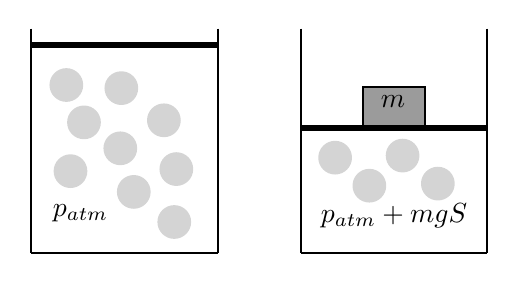
\begin{tikzpicture}[x=0.75pt,y=0.75pt,yscale=-1,xscale=1]
	%uncomment if require: \path (0,300); %set diagram left start at 0, and has height of 300

	%Shape: Rectangle [id:dp14035139223234783] 
	\draw  [fill={rgb, 255:red, 155; green, 155; blue, 155 }  ,fill opacity=1 ] (290,120) -- (320,120) -- (320,140) -- (290,140) -- cycle ;
	%Straight Lines [id:da49681278948526053] 
	\draw    (130,92) -- (130,200) ;
	%Straight Lines [id:da4994473620807358] 
	\draw    (220,92) -- (220,200) ;
	%Straight Lines [id:da6387671993341548] 
	\draw    (130,200) -- (220,200) ;
	%Straight Lines [id:da08286092123994537] 
	\draw [line width=2.25]    (130,100) -- (220,100) ;
	%Straight Lines [id:da8841436304629093] 
	\draw    (260,92) -- (260,200) ;
	%Straight Lines [id:da868104119488712] 
	\draw    (350,92) -- (350,200) ;
	%Straight Lines [id:da6604958276683548] 
	\draw    (260,200) -- (350,200) ;
	%Straight Lines [id:da4733301466444775] 
	\draw [line width=2.25]    (260,140) -- (350,140) ;
	%Shape: Circle [id:dp847297195728026] 
	\draw  [draw opacity=0][fill={rgb, 255:red, 212; green, 212; blue, 212 }  ,fill opacity=1 ] (139,119.13) .. controls (139,114.64) and (142.64,111) .. (147.13,111) .. controls (151.61,111) and (155.25,114.64) .. (155.25,119.13) .. controls (155.25,123.61) and (151.61,127.25) .. (147.13,127.25) .. controls (142.64,127.25) and (139,123.61) .. (139,119.13) -- cycle ;
	%Shape: Circle [id:dp5074006468657941] 
	\draw  [draw opacity=0][fill={rgb, 255:red, 212; green, 212; blue, 212 }  ,fill opacity=1 ] (165.5,120.63) .. controls (165.5,116.14) and (169.14,112.5) .. (173.63,112.5) .. controls (178.11,112.5) and (181.75,116.14) .. (181.75,120.63) .. controls (181.75,125.11) and (178.11,128.75) .. (173.63,128.75) .. controls (169.14,128.75) and (165.5,125.11) .. (165.5,120.63) -- cycle ;
	%Shape: Circle [id:dp24582200119657371] 
	\draw  [draw opacity=0][fill={rgb, 255:red, 212; green, 212; blue, 212 }  ,fill opacity=1 ] (186,136.13) .. controls (186,131.64) and (189.64,128) .. (194.13,128) .. controls (198.61,128) and (202.25,131.64) .. (202.25,136.13) .. controls (202.25,140.61) and (198.61,144.25) .. (194.13,144.25) .. controls (189.64,144.25) and (186,140.61) .. (186,136.13) -- cycle ;
	%Shape: Circle [id:dp8148506207242139] 
	\draw  [draw opacity=0][fill={rgb, 255:red, 212; green, 212; blue, 212 }  ,fill opacity=1 ] (147.5,137.13) .. controls (147.5,132.64) and (151.14,129) .. (155.63,129) .. controls (160.11,129) and (163.75,132.64) .. (163.75,137.13) .. controls (163.75,141.61) and (160.11,145.25) .. (155.63,145.25) .. controls (151.14,145.25) and (147.5,141.61) .. (147.5,137.13) -- cycle ;
	%Shape: Circle [id:dp5047766488519425] 
	\draw  [draw opacity=0][fill={rgb, 255:red, 212; green, 212; blue, 212 }  ,fill opacity=1 ] (165,149.63) .. controls (165,145.14) and (168.64,141.5) .. (173.13,141.5) .. controls (177.61,141.5) and (181.25,145.14) .. (181.25,149.63) .. controls (181.25,154.11) and (177.61,157.75) .. (173.13,157.75) .. controls (168.64,157.75) and (165,154.11) .. (165,149.63) -- cycle ;
	%Shape: Circle [id:dp5204784668116911] 
	\draw  [draw opacity=0][fill={rgb, 255:red, 212; green, 212; blue, 212 }  ,fill opacity=1 ] (141,160.63) .. controls (141,156.14) and (144.64,152.5) .. (149.13,152.5) .. controls (153.61,152.5) and (157.25,156.14) .. (157.25,160.63) .. controls (157.25,165.11) and (153.61,168.75) .. (149.13,168.75) .. controls (144.64,168.75) and (141,165.11) .. (141,160.63) -- cycle ;
	%Shape: Circle [id:dp4567328025212567] 
	\draw  [draw opacity=0][fill={rgb, 255:red, 212; green, 212; blue, 212 }  ,fill opacity=1 ] (192,159.63) .. controls (192,155.14) and (195.64,151.5) .. (200.13,151.5) .. controls (204.61,151.5) and (208.25,155.14) .. (208.25,159.63) .. controls (208.25,164.11) and (204.61,167.75) .. (200.13,167.75) .. controls (195.64,167.75) and (192,164.11) .. (192,159.63) -- cycle ;
	%Shape: Circle [id:dp7972438623150406] 
	\draw  [draw opacity=0][fill={rgb, 255:red, 212; green, 212; blue, 212 }  ,fill opacity=1 ] (171.5,170.63) .. controls (171.5,166.14) and (175.14,162.5) .. (179.63,162.5) .. controls (184.11,162.5) and (187.75,166.14) .. (187.75,170.63) .. controls (187.75,175.11) and (184.11,178.75) .. (179.63,178.75) .. controls (175.14,178.75) and (171.5,175.11) .. (171.5,170.63) -- cycle ;
	%Shape: Circle [id:dp2794407603749758] 
	\draw  [draw opacity=0][fill={rgb, 255:red, 212; green, 212; blue, 212 }  ,fill opacity=1 ] (191,185.13) .. controls (191,180.64) and (194.64,177) .. (199.13,177) .. controls (203.61,177) and (207.25,180.64) .. (207.25,185.13) .. controls (207.25,189.61) and (203.61,193.25) .. (199.13,193.25) .. controls (194.64,193.25) and (191,189.61) .. (191,185.13) -- cycle ;
	%Shape: Circle [id:dp5580122495464388] 
	\draw  [draw opacity=0][fill={rgb, 255:red, 212; green, 212; blue, 212 }  ,fill opacity=1 ] (268.5,154.13) .. controls (268.5,149.64) and (272.14,146) .. (276.63,146) .. controls (281.11,146) and (284.75,149.64) .. (284.75,154.13) .. controls (284.75,158.61) and (281.11,162.25) .. (276.63,162.25) .. controls (272.14,162.25) and (268.5,158.61) .. (268.5,154.13) -- cycle ;
	%Shape: Circle [id:dp49522420372510156] 
	\draw  [draw opacity=0][fill={rgb, 255:red, 212; green, 212; blue, 212 }  ,fill opacity=1 ] (301,153.13) .. controls (301,148.64) and (304.64,145) .. (309.13,145) .. controls (313.61,145) and (317.25,148.64) .. (317.25,153.13) .. controls (317.25,157.61) and (313.61,161.25) .. (309.13,161.25) .. controls (304.64,161.25) and (301,157.61) .. (301,153.13) -- cycle ;
	%Shape: Circle [id:dp966021302774063] 
	\draw  [draw opacity=0][fill={rgb, 255:red, 212; green, 212; blue, 212 }  ,fill opacity=1 ] (318,166.63) .. controls (318,162.14) and (321.64,158.5) .. (326.13,158.5) .. controls (330.61,158.5) and (334.25,162.14) .. (334.25,166.63) .. controls (334.25,171.11) and (330.61,174.75) .. (326.13,174.75) .. controls (321.64,174.75) and (318,171.11) .. (318,166.63) -- cycle ;
	%Shape: Circle [id:dp11574108347735068] 
	\draw  [draw opacity=0][fill={rgb, 255:red, 212; green, 212; blue, 212 }  ,fill opacity=1 ] (285,167.63) .. controls (285,163.14) and (288.64,159.5) .. (293.13,159.5) .. controls (297.61,159.5) and (301.25,163.14) .. (301.25,167.63) .. controls (301.25,172.11) and (297.61,175.75) .. (293.13,175.75) .. controls (288.64,175.75) and (285,172.11) .. (285,167.63) -- cycle ;

	% Text Node
	\draw (304.5,127) node    {$m$};
	% Text Node
	\draw (154,181) node    {$p_{atm}$};
	% Text Node
	\draw (305,182) node    {$p_{atm} +mgS$};

	\end{tikzpicture}
\end{figure}
\FloatBarrier
Il tempo non compare esplicitamente, a differenza di quanto avviene in meccanica. Durante la trasformazione termodinamica, il sistema scambierà energia con l'ambiente circostante.
Le trasformazioni termodinamiche si distinguono in due tipologie:

\begin{itemize}
	\item reversibili: sono quelle trasformazioni in cui è possibile tornare indietro allo stato di partenza scambiando esattamente le stesse quantità di energia ribaltate di segno. Si tratta in realtà di processi ideali.
	\item Irreversibili: sono quelle trasformazioni in cui non si verificano le condizioni precedenti, ossia che passano attraverso stati di non equilibrio e/o avvengono in presenza di forze dissipative o entrambe le cose.
\end{itemize}

Per realizzare una trasformazione in maniera reversibile essa deve essere prima di tutto \textbf{quasi statica}. Ciò significa che viene fatta avvenire per passaggi tra continui stati di equilibrio. La si fa avvenire così lentamente che il sistema va in un nuovo stato di equilibrio, lo si smuove un po' e lo si fa passare per un altro stato di equilibrio e via dicendo. In ogni punto della trasformazione quasi statica vale la funzione di stato. In aggiunta, perché essa sia reversibile, è necessario che durante la trasformazione tutti gli effetti dissipativi, ossia tutte le forze d'attrito, siano rimossi. Questo accade perché bisogna poter tornare indietro scambiando le stessa quantità di energia, quindi essa non può andare dissipata.
In una trasformazione reversibile, poiché passa per continui stati di equilibrio, i valori delle variabili termodinamiche sono noti in tutti i punti perché dati dalla funzione di stato, che è, proprio per la quasi staticità, valida in ogni istante. Ecco perché essa può essere graficata nel cosiddetto \textbf{piano di Clapeyron} come una certa funzione nelle variabili.

\begin{figure}[htpb]
	\centering

	\tikzset{every picture/.style={line width=0.75pt}} %set default line width to 0.75pt        

	\begin{tikzpicture}[x=0.75pt,y=0.75pt,yscale=-1,xscale=1]
	%uncomment if require: \path (0,300); %set diagram left start at 0, and has height of 300

	%Shape: Axis 2D [id:dp3310228244561544] 
	\draw  (148.5,177.74) -- (378.5,177.74)(159.52,101) -- (159.52,186) (371.5,172.74) -- (378.5,177.74) -- (371.5,182.74) (154.52,108) -- (159.52,101) -- (164.52,108)  ;

	% Text Node
	\draw (147,104.5) node    {$p$};
	% Text Node
	\draw (392.5,178) node    {$V$};

	\end{tikzpicture}
\end{figure}
\FloatBarrier
In una trasformazione irreversibile, sono noti stato iniziale e finale perché ivi è soddisfatta l'equazione di stato, ma in mezzo il gas assume valori caotici di volume pressione e temperatura, non noti. In questo caso si disegna la trasformazione tratteggiata.

\subsection{Lavoro meccanico}

Data una certa trasformazione, per passare da uno stato di equilibrio all'altro il sistema scambierà delle energie con l'ambiente circostanze. Esse potranno essere un lavoro meccanico, elettrico o un'energia termica.
La pressione è quella variabile che permette di capire se il sistema è in equilibrio meccanico con l'ambiente circostante. La mancanza di equilibrio meccanico comporta la realizzazione di un lavoro meccanico $\mathcal{L}$ chiamato lavoro della pressione.
Si immagini di voler calcolare il lavoro fatto dalla pressione di un gas in un cilindro mentre esso si espande di un tratto $z$, dalla situazione iniziale fino a quella finale.

\begin{figure}[htpb]
	\centering

	\tikzset{every picture/.style={line width=0.75pt}} %set default line width to 0.75pt        

	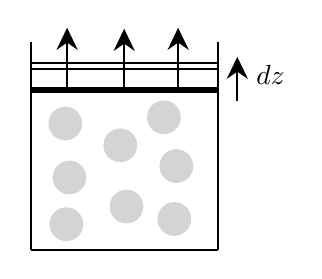
\begin{tikzpicture}[x=0.75pt,y=0.75pt,yscale=-1,xscale=1]
	%uncomment if require: \path (0,300); %set diagram left start at 0, and has height of 300

	%Straight Lines [id:da46135479872599006] 
	\draw    (130,100) -- (130,200) ;
	%Straight Lines [id:da5457765796068568] 
	\draw    (220,100) -- (220,200) ;
	%Straight Lines [id:da6748695752601523] 
	\draw    (130,200) -- (220,200) ;
	%Straight Lines [id:da5142681174243358] 
	\draw [line width=2.25]    (130,123) -- (220,123) ;
	%Shape: Circle [id:dp9738521381170515] 
	\draw  [draw opacity=0][fill={rgb, 255:red, 212; green, 212; blue, 212 }  ,fill opacity=1 ] (138.5,139.13) .. controls (138.5,134.64) and (142.14,131) .. (146.63,131) .. controls (151.11,131) and (154.75,134.64) .. (154.75,139.13) .. controls (154.75,143.61) and (151.11,147.25) .. (146.63,147.25) .. controls (142.14,147.25) and (138.5,143.61) .. (138.5,139.13) -- cycle ;
	%Shape: Circle [id:dp6699148200404468] 
	\draw  [draw opacity=0][fill={rgb, 255:red, 212; green, 212; blue, 212 }  ,fill opacity=1 ] (186,136.13) .. controls (186,131.64) and (189.64,128) .. (194.13,128) .. controls (198.61,128) and (202.25,131.64) .. (202.25,136.13) .. controls (202.25,140.61) and (198.61,144.25) .. (194.13,144.25) .. controls (189.64,144.25) and (186,140.61) .. (186,136.13) -- cycle ;
	%Shape: Circle [id:dp06833473002119006] 
	\draw  [draw opacity=0][fill={rgb, 255:red, 212; green, 212; blue, 212 }  ,fill opacity=1 ] (140.5,165.13) .. controls (140.5,160.64) and (144.14,157) .. (148.63,157) .. controls (153.11,157) and (156.75,160.64) .. (156.75,165.13) .. controls (156.75,169.61) and (153.11,173.25) .. (148.63,173.25) .. controls (144.14,173.25) and (140.5,169.61) .. (140.5,165.13) -- cycle ;
	%Shape: Circle [id:dp4991812434962075] 
	\draw  [draw opacity=0][fill={rgb, 255:red, 212; green, 212; blue, 212 }  ,fill opacity=1 ] (165,149.63) .. controls (165,145.14) and (168.64,141.5) .. (173.13,141.5) .. controls (177.61,141.5) and (181.25,145.14) .. (181.25,149.63) .. controls (181.25,154.11) and (177.61,157.75) .. (173.13,157.75) .. controls (168.64,157.75) and (165,154.11) .. (165,149.63) -- cycle ;
	%Shape: Circle [id:dp1471771351523674] 
	\draw  [draw opacity=0][fill={rgb, 255:red, 212; green, 212; blue, 212 }  ,fill opacity=1 ] (139,187.63) .. controls (139,183.14) and (142.64,179.5) .. (147.13,179.5) .. controls (151.61,179.5) and (155.25,183.14) .. (155.25,187.63) .. controls (155.25,192.11) and (151.61,195.75) .. (147.13,195.75) .. controls (142.64,195.75) and (139,192.11) .. (139,187.63) -- cycle ;
	%Shape: Circle [id:dp4476354313067108] 
	\draw  [draw opacity=0][fill={rgb, 255:red, 212; green, 212; blue, 212 }  ,fill opacity=1 ] (192,159.63) .. controls (192,155.14) and (195.64,151.5) .. (200.13,151.5) .. controls (204.61,151.5) and (208.25,155.14) .. (208.25,159.63) .. controls (208.25,164.11) and (204.61,167.75) .. (200.13,167.75) .. controls (195.64,167.75) and (192,164.11) .. (192,159.63) -- cycle ;
	%Shape: Circle [id:dp3622533136691808] 
	\draw  [draw opacity=0][fill={rgb, 255:red, 212; green, 212; blue, 212 }  ,fill opacity=1 ] (168,179.13) .. controls (168,174.64) and (171.64,171) .. (176.13,171) .. controls (180.61,171) and (184.25,174.64) .. (184.25,179.13) .. controls (184.25,183.61) and (180.61,187.25) .. (176.13,187.25) .. controls (171.64,187.25) and (168,183.61) .. (168,179.13) -- cycle ;
	%Shape: Circle [id:dp3062247486090506] 
	\draw  [draw opacity=0][fill={rgb, 255:red, 212; green, 212; blue, 212 }  ,fill opacity=1 ] (191,185.13) .. controls (191,180.64) and (194.64,177) .. (199.13,177) .. controls (203.61,177) and (207.25,180.64) .. (207.25,185.13) .. controls (207.25,189.61) and (203.61,193.25) .. (199.13,193.25) .. controls (194.64,193.25) and (191,189.61) .. (191,185.13) -- cycle ;
	%Straight Lines [id:da25081709908699445] 
	\draw [line width=0.75]    (130,110) -- (220,110)(130,113) -- (220,113) ;
	%Straight Lines [id:da5784681561768281] 
	\draw    (229.5,110) -- (229.5,128.5) ;
	\draw [shift={(229.5,107)}, rotate = 90] [fill={rgb, 255:red, 0; green, 0; blue, 0 }  ][line width=0.08]  [draw opacity=0] (10.72,-5.15) -- (0,0) -- (10.72,5.15) -- (7.12,0) -- cycle    ;
	%Straight Lines [id:da8294208051947267] 
	\draw    (147.5,96) -- (147.5,122.5) ;
	\draw [shift={(147.5,93)}, rotate = 90] [fill={rgb, 255:red, 0; green, 0; blue, 0 }  ][line width=0.08]  [draw opacity=0] (10.72,-5.15) -- (0,0) -- (10.72,5.15) -- (7.12,0) -- cycle    ;
	%Straight Lines [id:da9530121924947981] 
	\draw    (175,96.5) -- (175,123) ;
	\draw [shift={(175,93.5)}, rotate = 90] [fill={rgb, 255:red, 0; green, 0; blue, 0 }  ][line width=0.08]  [draw opacity=0] (10.72,-5.15) -- (0,0) -- (10.72,5.15) -- (7.12,0) -- cycle    ;
	%Straight Lines [id:da5497785411174465] 
	\draw    (201,96) -- (201,122.5) ;
	\draw [shift={(201,93)}, rotate = 90] [fill={rgb, 255:red, 0; green, 0; blue, 0 }  ][line width=0.08]  [draw opacity=0] (10.72,-5.15) -- (0,0) -- (10.72,5.15) -- (7.12,0) -- cycle    ;

	% Text Node
	\draw (245.5,115.5) node    {$dz$};

	\end{tikzpicture}
\end{figure}
\FloatBarrier
La forza che compie il lavoro è quella generata dalla pressione. In quanto tale, è sempre ortogonale al pistone, alla superficie su cui agisce. Il prodotto scalare $\vec{F}\cdot d\vec{r}$ sarà semplicemente il prodotto della forza normale per lo spostamento infinitesimo $dz$.

\[
	\mathcal{L} = \int \vec{F} d\vec{r} = \int F_n dz = \int p_{\text{gas} }Sdz
\]
$S$ è la superficie del pistone, e quindi $S\,dz$ è la variazione di volume infinitesima che subisce il gas mentre si espande. Il lavoro della pressione si può scrivere semplicemente come:

\[
	\boxed{\mathcal{L} = \int p_{\text{gas}}dV}
\]

La pressione del gas non è necessariamente costante. Ma se esso si espande la pressione diminuirà. Inoltre non è una variabile sempre nota durante la trasformazione. Lo è se la trasformazione è quasi statica. Quando non si ha un equilibrio delle pressioni, il gas fa sempre un lavoro meccanico legato alla pressione. In termodinamica ci si pone dal punto di vista del sistema termodinamico, cioè del gas. Il lavoro sarà positivo quando il gas si espande, è negativo altrimenti.

\subsection{Calore scambiato}

L'altra grandezza energetica che scambia il sistema termodinamico è il calore (si misura in Joule) e il suo scambio comporta movimenti macroscopici. La variabile termodinamica coinvolta è la temperatura. Essa è indice dell'equilibro termodinamico tra due corpi o fra il sistema termodinamico e l'ambiente circostante. Quando due corpi sono alla stessa temperatura, si dice che sono in equilibrio termico, altrimenti vi è passaggio di calore dal corpo più caldo al corpo più freddo. La scala termometrica che si usa nel sistema internazionale delle unità di misura è la scala Kelvin. Molto utilizzata è anche la scala Celsius, che è definita tramite due punti di riferimento: il punto di congelamento dell'acqua alla pressione atmosferica $(0 \degree \text{C})$ e quello della sua ebollizione (sempre alla pressione atmosferica, $100 \degree \text{C}$). Si prendono questi due punti, li si divide in cento parti e si ottiene la definizione di grado centigrado. La scala in gradi Kelvin invece è costruita in maniera tale che $0 \degree \text{C} =273.15 K$. Vi è poi una temperatura minima a cui un corpo può solo tendere che è proprio $0 K (-273.15 \degree \text{C})$. Le temperature in Kelvin sono quindi sempre positive. Quando le grandezze sono funzione del salto termico è equivalente usare i gradi centigradi o i Kelvin: aumentare o diminuire la temperatura di un grado Kelvin o Celsius è infatti la stessa cosa.

Quando due corpi sono a temperature diverse si può verificare uno scambio di calore che dipende da come essi sono fatti. Per caratterizzare la capacità che ha un materiale di variare la sua temperatura al variare dell'energia termica che assorbe, viene definita una grandezza caratteristica del materiale che prende il nome di \textbf{calore specifico} ($c$) e che fondamentalmente è un energia per unità di massa, per unità di temperatura. È definito come la quantità di energia termica, di calore, che bisogna fornire a un corpo per unità di massa per fargli variare la sua temperatura di una quantità infinitesima $dT$. È evidente che maggiore è il calore specifico, maggiore calore deve essere ceduto a pari salto termico.

\[
	c = \frac{1}{m} \frac{dQ}{dT}
\]

Calore specifico elevato vuole dire bassa capacità di variare la propria temperatura, bassa conducibilità termica. Basso calore specifico è tipico invece dei metalli. Dimensionalmente il calore specifico è:

\begin{gather*}
	c = \frac{[E]}{[m][T]} = \frac{J}{kg\cdot K} \\
	c_{H_2 O} = \frac{1\,cal }{g\, \degree \text{C} } = \frac{4.18 \, J}{g\, \degree \text{C}} = \frac{4180J}{kg\, \degree \text{C}}
\end{gather*}

Preso un grammo d'acqua, se si vuole innalzare la sua temperatura da $17.5 \degree \text{C}$ a $18.5 \degree \text{C}$ bisogna fornirgli una caloria o $4.18 \, J$.
Si usa la definizione di $c$ per ottenere quella di calore trasferito da un corpo all'altro. È possibile ribaltare la relazione e dire che l'energia termica che deve assorbire o cedere un corpo di massa $m$ e calore specifico $c$, a cui si vuol far aumentare la temperatura di una variazione infinitesima $dT$ è pari a:

\[
	dQ = m\,c\,dT
\]

Questa è una quantità infinitesima. Se si vuole la quantità totale di calore o di energia termica che è necessario fornire a un corpo per fargli variare la temperatura, si sommano in maniera continua tutti i calori infinitesimi, si calcola un integrale.

\[
	Q = \int_{T_A}^{T_B} m\,c\,dT
\]

Questa definizione è valida tutte le volte che il corpo non sta cambiando di fase. Quando una sostanza cambia fase non varia la sua temperatura, ma il calore specifico è diverso. Teoricamente bisognerebbe conoscere la funzione che descrive come varia $c$ al variare di $T$. Si ipotizzerà sempre costante il calore specifico nell'intervallo termico considerato. È evidente che quando il corpo si scalda l'energia sarà assorbita e quindi positiva.

Si supponga di avere una quantità di latte (1) che si vuole mischiare con del caffè liquido (2) in una tazza isolante, tale per cui gli scambi di calore con l'ambiente esterno sono trascurabili.

\begin{figure}[htpb]
	\centering

	\tikzset{every picture/.style={line width=0.75pt}} %set default line width to 0.75pt        

	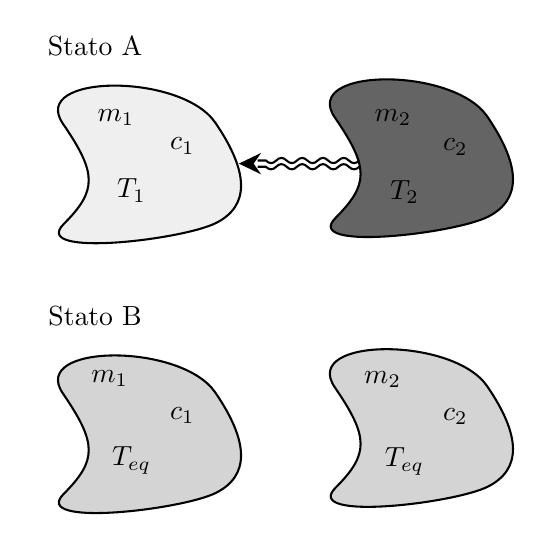
\begin{tikzpicture}[x=0.75pt,y=0.75pt,yscale=-1,xscale=1]
	%uncomment if require: \path (0,300); %set diagram left start at 0, and has height of 300

	%Shape: Regular Polygon [id:dp4011525611692206] 
	\draw  [fill={rgb, 255:red, 240; green, 239; blue, 239 }  ,fill opacity=1 ] (276.21,139.12) .. controls (259.96,147.3) and (186.65,155.91) .. (202.83,139.65) .. controls (219.02,123.4) and (218.96,115.33) .. (202.48,91.25) .. controls (186,67.16) and (259.37,66.63) .. (275.85,90.71) .. controls (292.33,114.79) and (292.45,130.93) .. (276.21,139.12) -- cycle ;
	%Shape: Regular Polygon [id:dp3359698689255244] 
	\draw  [fill={rgb, 255:red, 100; green, 100; blue, 100 }  ,fill opacity=1 ] (407.22,136.12) .. controls (390.97,144.31) and (317.63,152.92) .. (333.82,136.66) .. controls (350.01,120.4) and (349.95,112.33) .. (333.46,88.24) .. controls (316.98,64.15) and (390.37,63.61) .. (406.86,87.7) .. controls (423.35,111.79) and (423.47,127.93) .. (407.22,136.12) -- cycle ;
	%Straight Lines [id:da851480115804305] 
	\draw    (345.25,112) .. controls (343.58,113.67) and (341.92,113.67) .. (340.25,112) .. controls (338.58,110.33) and (336.92,110.33) .. (335.25,112) .. controls (333.58,113.67) and (331.92,113.67) .. (330.25,112) .. controls (328.58,110.33) and (326.92,110.33) .. (325.25,112) .. controls (323.58,113.67) and (321.92,113.67) .. (320.25,112) .. controls (318.58,110.33) and (316.92,110.33) .. (315.25,112) .. controls (313.58,113.67) and (311.92,113.67) .. (310.25,112) .. controls (308.58,110.33) and (306.92,110.33) .. (305.25,112) .. controls (303.58,113.67) and (301.92,113.67) .. (300.25,112) -- (299.25,112) -- (296.25,112)(345.25,109) .. controls (343.58,110.67) and (341.92,110.67) .. (340.25,109) .. controls (338.58,107.33) and (336.92,107.33) .. (335.25,109) .. controls (333.58,110.67) and (331.92,110.67) .. (330.25,109) .. controls (328.58,107.33) and (326.92,107.33) .. (325.25,109) .. controls (323.58,110.67) and (321.92,110.67) .. (320.25,109) .. controls (318.58,107.33) and (316.92,107.33) .. (315.25,109) .. controls (313.58,110.67) and (311.92,110.67) .. (310.25,109) .. controls (308.58,107.33) and (306.92,107.33) .. (305.25,109) .. controls (303.58,110.67) and (301.92,110.67) .. (300.25,109) -- (299.25,109) -- (296.25,109) ;
	\draw [shift={(287.25,110.5)}, rotate = 360] [fill={rgb, 255:red, 0; green, 0; blue, 0 }  ][line width=0.08]  [draw opacity=0] (10.72,-5.15) -- (0,0) -- (10.72,5.15) -- (7.12,0) -- cycle    ;
	%Shape: Regular Polygon [id:dp19706115012076286] 
	\draw  [fill={rgb, 255:red, 212; green, 212; blue, 212 }  ,fill opacity=1 ] (276.21,269.12) .. controls (259.96,277.3) and (186.65,285.91) .. (202.83,269.65) .. controls (219.02,253.4) and (218.96,245.33) .. (202.48,221.25) .. controls (186,197.16) and (259.37,196.63) .. (275.85,220.71) .. controls (292.33,244.79) and (292.45,260.93) .. (276.21,269.12) -- cycle ;
	%Shape: Regular Polygon [id:dp013310898503069435] 
	\draw  [fill={rgb, 255:red, 212; green, 212; blue, 212 }  ,fill opacity=1 ] (407.22,266.12) .. controls (390.97,274.31) and (317.63,282.92) .. (333.82,266.66) .. controls (350.01,250.4) and (349.95,242.33) .. (333.46,218.24) .. controls (316.98,194.15) and (390.37,193.61) .. (406.86,217.7) .. controls (423.35,241.79) and (423.47,257.93) .. (407.22,266.12) -- cycle ;

	% Text Node
	\draw (228,88.25) node    {$m_{1}$};
	% Text Node
	\draw (260,102) node    {$c_{1}$};
	% Text Node
	\draw (235.5,123.5) node    {$T_{1}$};
	% Text Node
	\draw (361.5,88.25) node    {$m_{2}$};
	% Text Node
	\draw (391.5,102.5) node    {$c_{2}$};
	% Text Node
	\draw (367,124) node    {$T_{2}$};
	% Text Node
	\draw (218,54) node   [align=left] {Stato A};
	% Text Node
	\draw (225,214) node    {$m_{1}$};
	% Text Node
	\draw (260,232) node    {$c_{1}$};
	% Text Node
	\draw (235.5,253.5) node    {$T_{eq}$};
	% Text Node
	\draw (356.5,214.5) node    {$m_{2}$};
	% Text Node
	\draw (391.5,232.5) node    {$c_{2}$};
	% Text Node
	\draw (367,254) node    {$T_{eq}$};
	% Text Node
	\draw (218,184) node   [align=left] {Stato B};

	\end{tikzpicture}
\end{figure}
\FloatBarrier
L'unico scambio termico che avviene è il passaggio di calore dal corpo più caldo al corpo più freddo. Si ipotizza che non ci sia lavoro meccanico perché ne il caffè ne il latte si espandono. Per capire come il sistema termodinamico arriva, dopo un certo tempo, in una situazione finale in cui i due corpi sono in equilibrio basta imporre che il calore totale scambiato nel sistema termodinamico è zero. Il corpo più freddo assorbe una quantità di calore $Q_1$ esattamente uguale a quella ceduta dal corpo più caldo, $Q_2$.

\begin{gather*}
	m_1 c_1 (T_{eq} - T_1 ) + m_2 c_2(T_{eq}-T_2) = 0 \\
	\boxed{T_{eq} = \frac{m_1 c_1 T_1 + m_2 c_2 T_2}{m_1 c_1+m_2 c_2}}
\end{gather*}

Questo risultato si ottiene nell'ipotesi che i calori specifici siano costanti al variare della temperatura e che durante il processo non avvenga nessun cambiamento di fase.
Insieme a $c$ si introduce il concetto di \textbf{capacità termica} di un oggetto. Essa è definita come il calore specifico del materiale di cui il corpo è costituito, per la sua massa. Dimensionalmente è un'energia su una temperatura e si misura in $J/K$.

È possibile che avvenga uno scambio di energia termica anche quando il corpo non cambia temperatura. Questo avviene quando sta cambiando di fase.

\begin{table}[htpb]
	\centering
	\begin{tabular}{ll}
		fusione & solido $\to$ liquido \\
		solidificazione & liquido $\to$ solido \\
		evaporazione & liquido $\to$ gassoso \\
		condensazione & gassoso $\to$ liquido \\
		sublimazione & solido $\to$ gassoso \\
		brinamento & gassoso $\to$ solido \\
	\end{tabular}
\end{table}

Se si va a guardare il microscopico, quando si ha un cambiamento di fase, ad esempio la fusione, l'energia fornita va a rompere alcuni legami molecolari. Per una sostanza in fase solida infatti, si hanno dei legami molecolari molto più rigidi di quelli che caratterizzerebbero la stessa sostanza liquida. Fino a che tutte le particelle della sostanza non sono state trasformate nella nuova fase, il corpo non cambia di temperatura. Si parla di processi ipotermici.
Non si avrà dipendenza da temperatura come in precedenza, ma solo dalla quantità di sostanza a cui si vuole far cambiare la fase e da un parametro detto \textbf{calore latente}. Esso dipende dal materiale in questione e dalla transizione di fase da seguire.

\[
	Q = m \lambda \qquad \lambda_s,\lambda_f,\lambda_v
\]

Cambiando verso $\lambda$ non cambia se non di segno. Se si vuole fondere una sostanza solida bisognerà fornire energia e quindi $\lambda$ sarà positivo, negativo altrimenti. Il calore latente dimensionalmente è un'energia per unità di massa e si misura come $J/kg$.

\paragraph{Osservazione} Una caratteristica molto importante dei cambiamenti di fase è di essere, in opportune condizioni, trasformazioni praticamente reversibili.

Si va a ridefinire il calore scambiato quando la sostanza è un gas: non si ha più il calore specifico per unità di massa ma il \textbf{calore specifico molare}, per unità di mole. Esso è la quantità di energia termica che deve assorbire o cedere un materiale durante la variazione di temperatura per unità di temperatura per numero di moli. Quando si ha a che fare con una sostanza in fase gassosa infatti la quantità di materia che c'è nel recipiente che contiene il gas viene data in numero di moli, quindi in numero di particelle contenute. Quest'ultimo generalmente è enorme. Una mole è un numero di particelle pari al \textbf{numero di Avogadro}, corrispondente al numero di atomi contenuti in $12 g$ dell'isotopo 12 del carbonio.

\[
	N_A = 6.022 \times 10^{23} \quad \text{particelle/mol}
\]

A seconda della specie molecolare, parlare di mole vuole dire avere un certo numero di atomi o di molecole.
In realtà il calore specifico è una grandezza che dipende dalla trasformazione $\Gamma$ che segue il gas, quando varia la sua temperatura. Si ha un certo valore del calore specifico quando si scalda un corpo a volume costante, oppure a pressione costante. In particolare si imparerà a definire il calore specifico di un gas quando viene scaldato a volume costante, $c_v$, mentre quello scambiato a pressione costante prende il nome di $c_p$. Si ha $c_p > c_v$ perché è più difficile scaldare un gas mantenendo la pressione costante piuttosto che a volume costante.

Ad esempio, per un gas monoatomico, specie stabile quando l'atomo è da solo, il calore specifico a volume costante è pari a $3/2\;R$ mentre a pressione costante è pari a $5/2\;R$ (dove $R$ è la costante universale dei gas). Per molti gas biatomici, soprattutto per quelle molecole disposte su una linea si ha:

\[
	c_v = \frac{5}{2}R \qquad c_p = \frac{7}{2}R
\]

\begin{table}[htpb]
	\centering
	\begin{tabular}{|c|c|c|}
		\hline
		gas & $c_p$ & $c_v$ \\
		\hline
		mono & $5/2 \;R$ & $3/2 \;R$ \\
		\hline
		bi & $7/2 \;R$ & $5/2 \;R$ \\
		\hline
	\end{tabular}
\end{table}

In realtà queste considerazioni su $c_p$ e $c_v$ sono vere anche per i liquidi e per i soldi, solo che quando una sostanza solida viene scaldata, si da per scontato che quella trasformazione stia avvenendo a pressione costante. In questo caso avviene una trasformazione isobara. Quello che si può notare al massimo è una leggera espansione del corpo. Ribaltando la definizione di calore specifico, si può calcolare il calore che scambia un grammo come l'integrale:

\[
	Q=\int n\,c_{\Gamma}dT = n\,c_{\Gamma}\Delta T
\]

\section{I principio della termodinamica}

Si consideri un sistema termodinamico costituito da un gas nello stato di equilibrio iniziale $A$ che in qualche maniera arriva a un nuovo stato di equilibrio finale $B$ seguendo un certo tipo di trasformazione $\Gamma_1$. Il gas scambierà una certa quantità di calore e una certa quantità di lavoro meccanico che dipenderanno dalla trasformazione seguita: si potrebbe infatti andare allo stesso stato finale seguendo diverse trasformazioni, a seconda delle quali esso scambierà determinate quantità di calore $Q$ e lavoro $\mathcal{L}$.

\begin{figure}[htpb]
	\centering

	\tikzset{every picture/.style={line width=0.75pt}} %set default line width to 0.75pt        

	\begin{tikzpicture}[x=0.75pt,y=0.75pt,yscale=-1,xscale=1]
	%uncomment if require: \path (0,300); %set diagram left start at 0, and has height of 300

	%Curve Lines [id:da6010533575144312] 
	\draw    (94,123) .. controls (134,93) and (174.5,256) .. (225.5,147) .. controls (276.5,38) and (291.5,176) .. (406.5,124) ;
	%Shape: Circle [id:dp19119229533280602] 
	\draw  [fill={rgb, 255:red, 0; green, 0; blue, 0 }  ,fill opacity=1 ] (91.75,123) .. controls (91.75,121.76) and (92.76,120.75) .. (94,120.75) .. controls (95.24,120.75) and (96.25,121.76) .. (96.25,123) .. controls (96.25,124.24) and (95.24,125.25) .. (94,125.25) .. controls (92.76,125.25) and (91.75,124.24) .. (91.75,123) -- cycle ;
	%Shape: Circle [id:dp532302755488802] 
	\draw  [fill={rgb, 255:red, 0; green, 0; blue, 0 }  ,fill opacity=1 ] (404.25,124) .. controls (404.25,122.76) and (405.26,121.75) .. (406.5,121.75) .. controls (407.74,121.75) and (408.75,122.76) .. (408.75,124) .. controls (408.75,125.24) and (407.74,126.25) .. (406.5,126.25) .. controls (405.26,126.25) and (404.25,125.24) .. (404.25,124) -- cycle ;

	% Text Node
	\draw (91,97) node    {$\text{stato di equilibrio} \ A$};
	% Text Node
	\draw (390,100) node    {$\text{stato di equilibrio} \ B$};
	% Text Node
	\draw (236,182) node    {$Q_{1} ,\mathcal{L}_{1}$};
	% Text Node
	\draw (264,89) node    {$\Gamma _{1}$};

	\end{tikzpicture}
\end{figure}
\FloatBarrier
Tuttavia, se si considera la quantità $Q-\mathcal{L}$, questa non dipende dalla trasformazione, ma solo dallo stato iniziale e finale.
Ciò significa che tale quantità è una funzione di stato, analogamente a come lo è l'energia potenziale. Si potrà sempre trovare una funzione $f$ tale per cui $Q-\mathcal{L}$ si può vedere come la variazione di $f$ valutata nello stato iniziale e in quello finale. La funzione prende il nome di \textbf{energia interna del sistema}.  Essa è definita a meno di una costante additiva, la cui presenza è irrilevante, in quanto dal punto di vista fisico è importante solo la sua variazione, come d'altronde nel caso dell'energia potenziale.

\begin{equation}
	\label{principio}
	\boxed{U(B)-U(A) = Q_p - \mathcal{L}_p \qquad U(m,T,p,V)}
\end{equation}

Si arriva così a enunciare il \textbf{primo principio della termodinamica}: esiste una funzione delle coordinate termodinamiche di un sistema, chiamata energia interna $U$, le cui variazioni generano gli scambi energetici del sistema con l'ambiente che lo circonda.

Tale principio è puramente sperimentale e rappresenta un bilancio energetico di un processo termodinamico. Non è altro che un principio di conservazione dell'energia in forma molto generale. L'energia intera accumulata in un sistema termodinamico è quella che può trasformarsi in lavoro meccanico della pressione, il quale a sua volta potrà trasformarsi in calore ceduto all'ambiente circostante. Essa può variare in modo da dare luogo a degli scambi di energia con l'ambiente circostante. Fisicamente essa racchiude tutti i contributi di energia cinetica e potenziale che ha il sistema termodinamico.
A livello microscopico, Un gas è costituito da tante particelle che si muovono secondo un moto di agitazione caotico che prende il nome di \textbf{agitazione termica}. Tali particelle forniscono un contributo di energia cinetica a $U$. L'agitazione termica è tanto più elevata quanto più è elevata la temperatura.
In più le molecole sono legate fra di loro da un legame che si può approssimare a una molla, e che figura in $U$ come contributo di energia potenziale della molla.
Si può collegare l'energia interna macroscopicamente al valore delle variabili termodinamiche e dire che quando un gas ha quei valori delle variabili ha quell'energia interna.
~\eqref{principio} è una relazione che collega un stato iniziale e finale distanti fra di loro, non infinitesima. La stessa relazione là si può scrivere anche come quantità infinitesime, andando a vedere quello che accade fra due stati molto vicini fra di loro.

\[
	dU = \delta Q - \delta\mathcal{L} \implies \int_A^B dU = \int_{\Gamma} \delta Q - \int_{\Gamma} \delta\mathcal{L}
\]

Questa cosa comunica che la quantità $dU$ infinitesima, a differenza di $\delta Q$ e $\delta\mathcal{L}$, è un \emph{differenziale esatto}. Significa che quando la si integra, si ha un integrale che non dipende dalla trasformazione.

\paragraph{Riassunto dei punti principali riguardo al primo principio della termodinamica}

\begin{itemize}
	\item Sperimentalmente si trova sempre verificato questo risultato: se il sistema compie una trasformazione dallo stato $A$ allo stato $B$, scambiando calore e lavoro con l'ambiente, $Q$ e $\mathcal{L}$ dipendono dalla trasformazione che congiunge i due stati termodinamici, mentre la loro differenza risulta indipendente dalla trasformazione.
	\item esiste una funzione delle coordinate termodinamiche del sistema o, come si dice, una funzione di stato, chiamata energia interna, le cui variazioni danno luogo a scambi energetici del sistema con l'ambiente che lo circonda durante una trasformazione.
	\item Quando, durante una trasformazione, si fornisce energia a un sistema, sia tramite un lavoro meccanico che con uno scambio di calore, questa resta immagazzinata sotto forma di energia interna e può essere successivamente
	utilizzata.
	\item Il termine energia interna indica che non si tratta dell'energia cinetica del sistema nel suo complesso, o dell'energia potenziale, bensì di un'energia legata alle proprietà interne del sistema, come moto molecolare o forze intermolecolari, che non dipendono dallo stato complessivo di moto, ma piuttosto dalla temperatura del sistema, dalla pressione a cui è sottoposto o dal volume che occupa.
	\item Il primo principio mette in evidenza l'esistenza di un meccanismo di scambio di energia, che non è esprimibile come lavoro meccanico macroscopico: a questo si da il nome di calore ed è ancora riconducibile a fenomeni meccanici, ma a livello microscopico. Il primo principio della termodinamica fornisce la definizione più generale di calore, sia concettualmente che dal punto di vista del calcolo.
\end{itemize}

Finora è stato definito come esprimere l'energia termica scambiata dal sistema termodinamico quando esso varia la sua temperatura o quando subisce un cambio di fase, oppure il lavoro se è di tipo meccanico, e quindi subito dalla pressione del gas. In realtà si potrebbe avere anche lavoro elettrico. Ad esempio se all'interno di un recipiente contenete un gas si fa passare una resistenza elettrica percorsa da corrente, viene compiuto lavoro elettrico dovuto al passaggio della corrente nel conduttore. La relazione comprende tutti i possibili lavori fatti o subiti dal gas.

Se si considera una trasformazione termodinamica ciclica, secondo il primo principio della dinamica:

\[
	\Delta U_{\text{ciclo} } = Q_{\Gamma,\text{ciclo} } -\mathcal{L}_{\Gamma,\text{ciclo} }  =0 \implies \mathcal{L}=Q
\]

\begin{figure}[htpb]
	\centering

	\tikzset{every picture/.style={line width=0.75pt}} %set default line width to 0.75pt        

	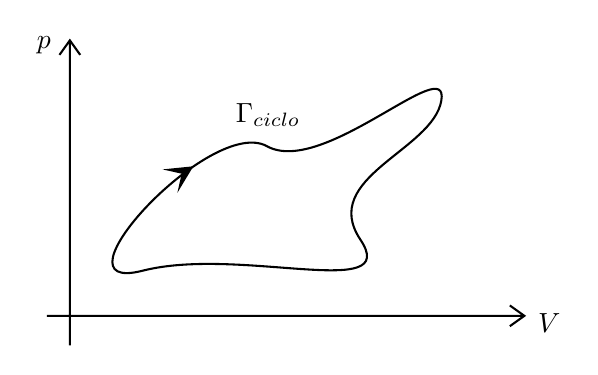
\begin{tikzpicture}[x=0.75pt,y=0.75pt,yscale=-1,xscale=1]
	%uncomment if require: \path (0,300); %set diagram left start at 0, and has height of 300

	%Shape: Axis 2D [id:dp6876434402516973] 
	\draw  (128.5,214.72) -- (358.5,214.72)(139.52,82) -- (139.52,229) (351.5,209.72) -- (358.5,214.72) -- (351.5,219.72) (134.52,89) -- (139.52,82) -- (144.52,89)  ;
	%Shape: Polygon Curved [id:ds34099068300713564] 
	\draw   (234.5,133) .. controls (261.5,148) and (322.5,87) .. (318.5,111) .. controls (314.5,135) and (259.5,148) .. (279.5,178) .. controls (299.5,208) and (221.5,181) .. (174.5,193) .. controls (127.5,205) and (207.5,118) .. (234.5,133) -- cycle ;
	\draw  [fill={rgb, 255:red, 0; green, 0; blue, 0 }  ,fill opacity=1 ] (187.3,144.36) -- (198.08,143.27) -- (192.49,152.55) -- (193.99,145.86) -- cycle ;

	% Text Node
	\draw (235,118) node    {$\Gamma _{\text{ciclo}}$};
	% Text Node
	\draw (127,84.5) node    {$p$};
	% Text Node
	\draw (370.5,218) node    {$V$};

	\end{tikzpicture}
\end{figure}
\FloatBarrier
L'energia interna è funzione solo dello stato iniziale, quindi qualunque processo si segua, la variazione dell'energia interna è sempre uguale a zero durante una trasformazione ciclica. Durante il ciclo il sistema termodinamico scambia calore e lavoro ma le due quantità energetiche scambiate si bilanciano, il lavoro scambiato è esattamente uguale al lavoro compiuto.

\section{I gas perfetti}

\subsection{Definizione e equazione di stato}

Un \textbf{gas perfetto} è un gas tale per cui le sue particelle interagiscono molto poco le une con le altre, non sono così vicine da essere attratte per attrazione elettrostatica o gravitazionale. Le uniche interazioni che subiscono saranno urti fra di loro e con le pareti del contenitore presente. Dal punto di vista delle variabili termodinamiche, per avere un gas perfetto bisogna essere in condizioni di pressione e temperatura tali per cui si è sufficientemente lontani dal punto di condensazione del gas. Le particelle sono tante ma c'è tanto spazio vuoto tra una molecola e l'altra. In questo paragrafo si definiscono delle relazioni che valgono soltanto quando si ha un gas perfetto o ideale.

Avendo a che fare con una sostanza in fase gassosa, le variabile termodinamiche adatte per descrivere lo stato di un gas sono:

\begin{itemize}
	\item La quantità di molecole o di particelle contenuta in un certo recipiente: il numero di moli
	\item La pressione
	\item La temperatura
	\item Il volume occupato dal gas
\end{itemize}

Vari esperimenti condotti da scienziati su gas perfetti dedussero quattro leggi sperimentali:

\begin{itemize}
	\item \textbf{Legge di Boyle}: se un gas viene mantenuto a temperatura costante, il prodotto pressione volume si mantiene constante;
	\[ \boxed{p_1 V_1=p_2 V_2} \]
	\item \textbf{Legge di espansione isobara, o di Volta-Gay-Lussac}. Se si mantiene il gas a pressione costante, scaldandolo il volume aumenta proporzionalmente con la sua temperatura.
	\[ \boxed{V=V_0(1+\alpha T) } \quad \alpha = \text{coefficiente di dilatazione termica} \]
	\item \textbf{Legge isocora di Gay-Lussac}: se si mantiene il volume costante, quindi si blocca il recipiente in cui è contenuto il gas, e lo si scalda, aumenterà la pressione. Il suo aumento è lineare con l'aumento di temperatura.
	\[ \boxed{p=p_0(1+\beta T) } \quad \beta = \text{coefficiente di espansione dei gas} \]
	\item \textbf{Legge di Avogadro}: volumi uguali di gas diversi, alla stessa temperatura e pressione, contengono lo stesso numero di molecole.
\end{itemize}

Da quest'ultima legge deriva la definizione di \textbf{volume molare}. Se si ha un gas qualunque e lo si porta alla pressione di un atmosfera e alla temperatura di $0 \degree \text{C}$, allora una mole di gas occuperà sempre un volume pari a $22.4$ litri. Questo risultato non dipende dal tipo di gas perché essendo perfetto è così rarefatto che lo spazio occupato dalle molecole è ininfluente. Il volume occupato dipende solo dal numero di moli.

Si definisce, sulla base delle tre leggi elementari e della legge di Avogadro, come gas ideale un sistema le cui coordinate termodinamiche in uno stato di equilibrio obbediscono all'\textbf{equazione di stato di un gas ideale}:

\[
	\boxed{pV=nRT} \qquad R=\frac{[p][L]^3}{[mol][K]}
\]

Dove $R$ è costante e vale $8.31 J/(K\,\text{mol})$.
La relazione la si può usare tutte le volte che il gas perfetto è in condizioni di equilibrio termodinamico.

\subsection{Trasformazioni termodinamiche di gas perfetti}

Si consideri una trasformazione che va da $A$ a $B$, stati di equilibrio. In tali punti le variabili termodinamiche del gas soddisferanno sempre l'equazione di stato. Nei punti intermedi della relazione non si può imporre la validità dell'equazione di stato.
La relazione mostra che le quattro variabili non sono indipendenti. Noto il numero di moli, allora la temperatura è automaticamente fissata, e bastano due variabili termodinamiche per conoscere completamente lo stato del sistema. Ecco perché è possibile utilizzare il piano di Clapeyron (che ha due soli assi) per definire uno stato termodinamico.

È stato detto che quando il gas si espande o si comprime, il lavoro fatto da esso lungo la trasformazione $\Gamma$ è quello dovuto alla pressione. La sua espressione è la seguente:

\[
	\mathcal{L}_{\Gamma} = \int_{\Gamma }\rho_{\text{gas} }dV
\]

Se la trasformazione è quasi statica, lungo tutti gli stati intermedi della trasformazione il gas soddisfa l'equazione di stato. La pressione del gas potrà essere riscritta in base alla relazione $pV=nRT$.

\[
	\mathcal{L}_{\Gamma }= \int \frac{nRT}{V}dV
\]

C'è un modo più semplice per calcolare il lavoro compiuto dal gas quando si espande secondo una trasformazione quasi statica. Se il piano di Clapeyron mette in relazione pressione volume, il lavoro è rappresentato dall'area sottesa dalla trasformazione, con segno positivo o negativo a seconda di espansione o compressione.
Viceversa, se la trasformazione non è quasi statica e quindi gli stati intermedi durante la trasformazione non sono noti, non si può imporre la validità dell'equazione di stato. Si sfrutta il fatto che se il gas nel pistone si sta espandendo, il lavoro che compie sarà subito dall'ambiente circostante. Tutta l'atmosfera subisce il lavoro, essa si trova ad una certa pressione e viene compressa. La pressione dell'atmosfera è sempre la stessa e quindi il lavoro sarà:

\[
	-\mathcal{L}_{est} = - p_{est}\Delta V
\]

Questo è un metodo molto efficace per calcolare il lavoro quando la trasformazione non è reversibile.

In seguito una classifica di alcune delle trasformazioni più importanti che si incontreranno.

\paragraph{Trasformazione isoterma} È una trasformazione che avviene a temperatura costante.

\[
	T=\text{costante} \implies pV=\text{costante}
\]
$pV=$cost rappresenta un'iperbole.

\begin{figure}[htpb]
	\centering

	\tikzset{every picture/.style={line width=0.75pt}} %set default line width to 0.75pt        

	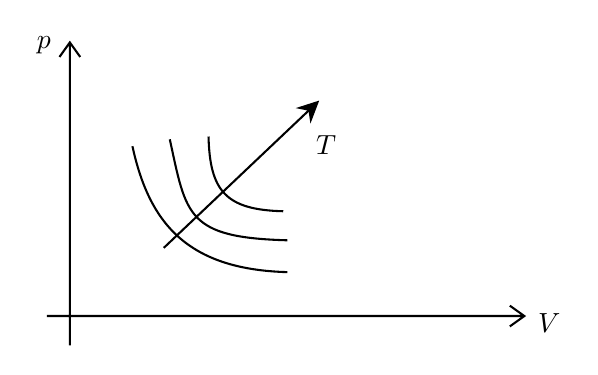
\begin{tikzpicture}[x=0.75pt,y=0.75pt,yscale=-1,xscale=1]
	%uncomment if require: \path (0,300); %set diagram left start at 0, and has height of 300

	%Shape: Axis 2D [id:dp3762397448703849] 
	\draw  (128.5,214.82) -- (358.5,214.82)(139.52,83) -- (139.52,229) (351.5,209.82) -- (358.5,214.82) -- (351.5,219.82) (134.52,90) -- (139.52,83) -- (144.52,90)  ;
	%Straight Lines [id:da7833866831656486] 
	\draw    (257.49,113.06) -- (184.75,182) ;
	\draw [shift={(259.67,111)}, rotate = 136.54] [fill={rgb, 255:red, 0; green, 0; blue, 0 }  ][line width=0.08]  [draw opacity=0] (10.72,-5.15) -- (0,0) -- (10.72,5.15) -- (7.12,0) -- cycle    ;
	%Curve Lines [id:da08665820907179822] 
	\draw    (169.67,133) .. controls (177.67,169.67) and (195.67,192.33) .. (244.33,193.67) ;
	%Curve Lines [id:da14814853449635912] 
	\draw    (187.67,129.67) .. controls (195.67,166.33) and (195.67,177) .. (244.33,178.33) ;
	%Curve Lines [id:da8569087873264798] 
	\draw    (206.33,128.33) .. controls (207,154.33) and (214.33,163.67) .. (242.33,164.33) ;

	% Text Node
	\draw (127,84.5) node    {$p$};
	% Text Node
	\draw (370.5,218) node    {$V$};
	% Text Node
	\draw (263,132.5) node    {$T$};

	\end{tikzpicture}
\end{figure}
\FloatBarrier
Questa, che porta dallo stato $A$ allo stato $B$ rappresenta la trasformazione isoterma di un gas, si va ad aumentare il volume a scapito della pressione che diminuisce. Se la si disegna continua la si intende reversibile, se la si fa tratteggiata è irreversibile. Aumentando la temperatura dell'isoterma, l'iperbole si sposta verso destra (si veda la figura). Tale osservazione aiuta molto a capire in altre trasformazioni se il gas si sta scaldando o raffreddando perché disegnare una famiglia di isoterme significa visualizzare sul piano di Clapeyron i luoghi dei punti a temperatura costante.

\paragraph{Trasformazione isobara} Si tratta di trasformazioni che avvengono a pressione costante. Si parte da uno stato $A$ e si arriva a uno stato $B$ tramite una retta. Il gas è tale per cui dallo stato $A$ passerà nella isoterma a sinistra, nello stato $B$ passerà per in isoterma più a destra, quindi il gas si scalda.

\begin{figure}[htpb]
	\centering

	\tikzset{every picture/.style={line width=0.75pt}} %set default line width to 0.75pt        

	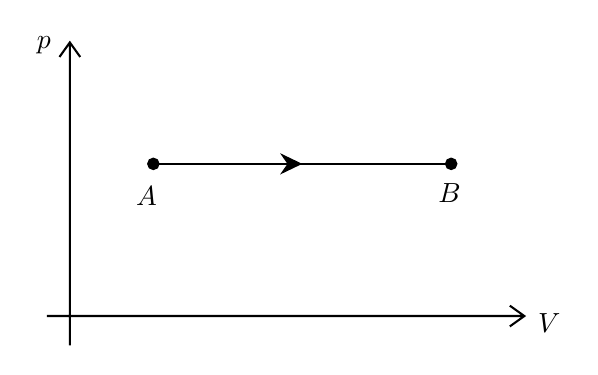
\begin{tikzpicture}[x=0.75pt,y=0.75pt,yscale=-1,xscale=1]
	%uncomment if require: \path (0,300); %set diagram left start at 0, and has height of 300

	%Shape: Axis 2D [id:dp33331390425563545] 
	\draw  (128.5,214.82) -- (358.5,214.82)(139.52,83) -- (139.52,229) (351.5,209.82) -- (358.5,214.82) -- (351.5,219.82) (134.52,90) -- (139.52,83) -- (144.52,90)  ;
	%Straight Lines [id:da8859151290369149] 
	\draw    (323.25,141.5) -- (179.75,141.5) ;
	\draw [shift={(251.5,141.5)}, rotate = 180] [fill={rgb, 255:red, 0; green, 0; blue, 0 }  ][line width=0.08]  [draw opacity=0] (10.72,-5.15) -- (0,0) -- (10.72,5.15) -- (7.12,0) -- cycle    ;
	%Shape: Circle [id:dp5063629402975616] 
	\draw  [fill={rgb, 255:red, 0; green, 0; blue, 0 }  ,fill opacity=1 ] (177.25,141.5) .. controls (177.25,140.12) and (178.37,139) .. (179.75,139) .. controls (181.13,139) and (182.25,140.12) .. (182.25,141.5) .. controls (182.25,142.88) and (181.13,144) .. (179.75,144) .. controls (178.37,144) and (177.25,142.88) .. (177.25,141.5) -- cycle ;
	%Shape: Circle [id:dp2755167660691369] 
	\draw  [fill={rgb, 255:red, 0; green, 0; blue, 0 }  ,fill opacity=1 ] (320.75,141.5) .. controls (320.75,140.12) and (321.87,139) .. (323.25,139) .. controls (324.63,139) and (325.75,140.12) .. (325.75,141.5) .. controls (325.75,142.88) and (324.63,144) .. (323.25,144) .. controls (321.87,144) and (320.75,142.88) .. (320.75,141.5) -- cycle ;

	% Text Node
	\draw (127,84.5) node    {$p$};
	% Text Node
	\draw (370.5,218) node    {$V$};
	% Text Node
	\draw (176.5,157) node    {$A$};
	% Text Node
	\draw (322.5,155.5) node    {$B$};

	\end{tikzpicture}
\end{figure}
\FloatBarrier

\paragraph{Trasformazione isocora} Si tratta di trasformazioni che avvengono a volume costante e sono graficate da una retta. Aumentando la pressione, aiutandosi sempre con i grafici delle isoterme, si vede che la temperatura aumenta e quindi il gas si riscalda (\emph{riscaldamento isocoro}).

\begin{figure}[htpb]
	\centering

	\tikzset{every picture/.style={line width=0.75pt}} %set default line width to 0.75pt        

	\begin{tikzpicture}[x=0.75pt,y=0.75pt,yscale=-1,xscale=1]
	%uncomment if require: \path (0,300); %set diagram left start at 0, and has height of 300

	%Shape: Axis 2D [id:dp9666306813741952] 
	\draw  (128.5,214.91) -- (358.5,214.91)(139.52,84) -- (139.52,229) (351.5,209.91) -- (358.5,214.91) -- (351.5,219.91) (134.52,91) -- (139.52,84) -- (144.52,91)  ;
	%Straight Lines [id:da2063233018113888] 
	\draw    (242.2,109) -- (242.2,197.25) ;
	\draw [shift={(242.2,153.12)}, rotate = 90] [fill={rgb, 255:red, 0; green, 0; blue, 0 }  ][line width=0.08]  [draw opacity=0] (10.72,-5.15) -- (0,0) -- (10.72,5.15) -- (7.12,0) -- cycle    ;
	%Shape: Circle [id:dp9362939801432519] 
	\draw  [fill={rgb, 255:red, 0; green, 0; blue, 0 }  ,fill opacity=1 ] (242.21,199.75) .. controls (240.82,199.75) and (239.7,198.63) .. (239.7,197.25) .. controls (239.7,195.87) and (240.82,194.75) .. (242.2,194.75) .. controls (243.58,194.75) and (244.7,195.87) .. (244.7,197.25) .. controls (244.7,198.63) and (243.59,199.75) .. (242.21,199.75) -- cycle ;
	%Shape: Circle [id:dp5098416031796373] 
	\draw  [fill={rgb, 255:red, 0; green, 0; blue, 0 }  ,fill opacity=1 ] (242.21,111.5) .. controls (240.82,111.5) and (239.7,110.38) .. (239.7,109) .. controls (239.7,107.62) and (240.82,106.5) .. (242.2,106.5) .. controls (243.58,106.5) and (244.7,107.62) .. (244.7,109) .. controls (244.7,110.38) and (243.59,111.5) .. (242.21,111.5) -- cycle ;

	% Text Node
	\draw (127,84.5) node    {$p$};
	% Text Node
	\draw (370.5,218) node    {$V$};
	% Text Node
	\draw (225.17,195.67) node    {$A$};
	% Text Node
	\draw (227.17,106.17) node    {$B$};

	\end{tikzpicture}
\end{figure}
\FloatBarrier

\paragraph{Trasformazione adiabatica} Sono quelle trasformazioni che avvengono senza scambi di calore con l'ambiente. In esse non viene bloccata una costante ma si impone $Q=0$.

Queste ovviamente non sono le uniche trasformazione che può subire il gas.

\subsection{Espressione dell'energia interna di un gas perfetto}

\paragraph{Espansione libera di un gas perfetto eseguita da Joule} Si prende un recipiente con pareti rigide e adiabatiche, ossia indeformabili e perfettamente isolanti. Il recipiente è diviso in due parti da un setto rigido che ha un'apertura chiusa da un rubinetto. In una delle camere si inserisce una certa quantità di un gas perfetto.
Nella seconda camera viene fatto il vuoto, si aspira tutta l'aria che eventualmente era presente, così da eliminare qualunque molecola: la pressione in tale camera è $0 atm$. Si apre il rubinetto e si lascia espandere il gas contro il vuoto. \emph{Espansione libera} si riferisce proprio al fatto che l'espansione avviene contro il nulla. Sperimentalmente si può andare a misurare quali sono i valori di volume pressione e temperatura e si trova che, se il gas è perfetto, comunque sia fatto l'esperimento, la temperatura finale del gas è esattamente uguale a quella iniziale. Per tale trasformazione si scrive allora il primo principio della termodinamica.

\[
	Q-\mathcal{L}=0 \implies \Delta U=0
\]

Il sistema infatti non scambia energia con l'ambiente, essendo le pareti rigide e adiabatiche. In tale processo termodinamico l'energia interna del gas non varia. Quella accumulata nello stato iniziale è uguale a quella accumulata nello stato finale. Si deduce quindi che $U$ non è funzione della pressione e del volume perché è rimasta la stessa nonostante essi sian variati. Allora è evidente che l'energia interna in un gas perfetto è funzione della temperatura, perché $T$ non è variata e di conseguenza nemmeno $U$.

\begin{figure}[htpb]
	\centering

	\tikzset{every picture/.style={line width=0.75pt}} %set default line width to 0.75pt        

	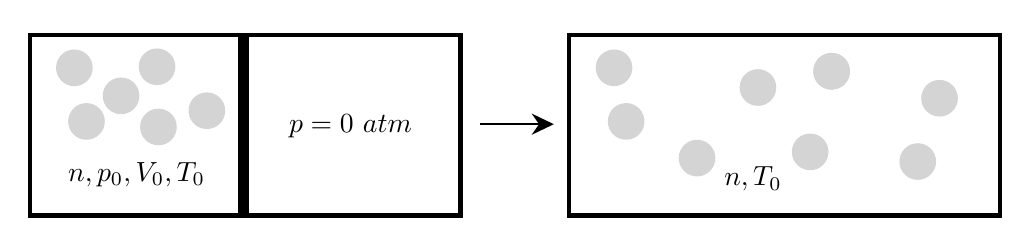
\begin{tikzpicture}[x=0.75pt,y=0.75pt,yscale=-1,xscale=1]
	%uncomment if require: \path (0,300); %set diagram left start at 0, and has height of 300

	%Shape: Rectangle [id:dp684426269344268] 
	\draw  [line width=1.5]  (132,71) -- (339.5,71) -- (339.5,158) -- (132,158) -- cycle ;
	%Straight Lines [id:da3693322295005539] 
	\draw [line width=3.75]    (235,70) -- (235,158) ;
	%Shape: Circle [id:dp2789327757534068] 
	\draw  [draw opacity=0][fill={rgb, 255:red, 212; green, 212; blue, 212 }  ,fill opacity=1 ] (144.67,86.83) .. controls (144.67,81.95) and (148.62,78) .. (153.5,78) .. controls (158.38,78) and (162.33,81.95) .. (162.33,86.83) .. controls (162.33,91.71) and (158.38,95.67) .. (153.5,95.67) .. controls (148.62,95.67) and (144.67,91.71) .. (144.67,86.83) -- cycle ;
	%Shape: Circle [id:dp4620531125360525] 
	\draw  [draw opacity=0][fill={rgb, 255:red, 212; green, 212; blue, 212 }  ,fill opacity=1 ] (184.5,86.33) .. controls (184.5,81.45) and (188.45,77.5) .. (193.33,77.5) .. controls (198.21,77.5) and (202.17,81.45) .. (202.17,86.33) .. controls (202.17,91.21) and (198.21,95.17) .. (193.33,95.17) .. controls (188.45,95.17) and (184.5,91.21) .. (184.5,86.33) -- cycle ;
	%Shape: Circle [id:dp2905872442111941] 
	\draw  [draw opacity=0][fill={rgb, 255:red, 212; green, 212; blue, 212 }  ,fill opacity=1 ] (208.5,107.5) .. controls (208.5,102.62) and (212.45,98.67) .. (217.33,98.67) .. controls (222.21,98.67) and (226.17,102.62) .. (226.17,107.5) .. controls (226.17,112.38) and (222.21,116.33) .. (217.33,116.33) .. controls (212.45,116.33) and (208.5,112.38) .. (208.5,107.5) -- cycle ;
	%Shape: Circle [id:dp14827622187931477] 
	\draw  [draw opacity=0][fill={rgb, 255:red, 212; green, 212; blue, 212 }  ,fill opacity=1 ] (150.5,112.67) .. controls (150.5,107.79) and (154.45,103.83) .. (159.33,103.83) .. controls (164.21,103.83) and (168.17,107.79) .. (168.17,112.67) .. controls (168.17,117.55) and (164.21,121.5) .. (159.33,121.5) .. controls (154.45,121.5) and (150.5,117.55) .. (150.5,112.67) -- cycle ;
	%Shape: Circle [id:dp02711217543111255] 
	\draw  [draw opacity=0][fill={rgb, 255:red, 212; green, 212; blue, 212 }  ,fill opacity=1 ] (167.17,100.33) .. controls (167.17,95.45) and (171.12,91.5) .. (176,91.5) .. controls (180.88,91.5) and (184.83,95.45) .. (184.83,100.33) .. controls (184.83,105.21) and (180.88,109.17) .. (176,109.17) .. controls (171.12,109.17) and (167.17,105.21) .. (167.17,100.33) -- cycle ;
	%Shape: Circle [id:dp09428837669637646] 
	\draw  [draw opacity=0][fill={rgb, 255:red, 212; green, 212; blue, 212 }  ,fill opacity=1 ] (185.17,115.33) .. controls (185.17,110.45) and (189.12,106.5) .. (194,106.5) .. controls (198.88,106.5) and (202.83,110.45) .. (202.83,115.33) .. controls (202.83,120.21) and (198.88,124.17) .. (194,124.17) .. controls (189.12,124.17) and (185.17,120.21) .. (185.17,115.33) -- cycle ;
	%Shape: Rectangle [id:dp45584182924648853] 
	\draw  [line width=1.5]  (392,71) -- (599.5,71) -- (599.5,158) -- (392,158) -- cycle ;
	%Shape: Circle [id:dp23771206303308867] 
	\draw  [draw opacity=0][fill={rgb, 255:red, 212; green, 212; blue, 212 }  ,fill opacity=1 ] (404.67,86.83) .. controls (404.67,81.95) and (408.62,78) .. (413.5,78) .. controls (418.38,78) and (422.33,81.95) .. (422.33,86.83) .. controls (422.33,91.71) and (418.38,95.67) .. (413.5,95.67) .. controls (408.62,95.67) and (404.67,91.71) .. (404.67,86.83) -- cycle ;
	%Shape: Circle [id:dp015976345398689862] 
	\draw  [draw opacity=0][fill={rgb, 255:red, 212; green, 212; blue, 212 }  ,fill opacity=1 ] (474,96.33) .. controls (474,91.45) and (477.95,87.5) .. (482.83,87.5) .. controls (487.71,87.5) and (491.67,91.45) .. (491.67,96.33) .. controls (491.67,101.21) and (487.71,105.17) .. (482.83,105.17) .. controls (477.95,105.17) and (474,101.21) .. (474,96.33) -- cycle ;
	%Shape: Circle [id:dp7875101498064774] 
	\draw  [draw opacity=0][fill={rgb, 255:red, 212; green, 212; blue, 212 }  ,fill opacity=1 ] (551,132) .. controls (551,127.12) and (554.95,123.17) .. (559.83,123.17) .. controls (564.71,123.17) and (568.67,127.12) .. (568.67,132) .. controls (568.67,136.88) and (564.71,140.83) .. (559.83,140.83) .. controls (554.95,140.83) and (551,136.88) .. (551,132) -- cycle ;
	%Shape: Circle [id:dp33350367514751666] 
	\draw  [draw opacity=0][fill={rgb, 255:red, 212; green, 212; blue, 212 }  ,fill opacity=1 ] (410.5,112.67) .. controls (410.5,107.79) and (414.45,103.83) .. (419.33,103.83) .. controls (424.21,103.83) and (428.17,107.79) .. (428.17,112.67) .. controls (428.17,117.55) and (424.21,121.5) .. (419.33,121.5) .. controls (414.45,121.5) and (410.5,117.55) .. (410.5,112.67) -- cycle ;
	%Shape: Circle [id:dp8197882534729368] 
	\draw  [draw opacity=0][fill={rgb, 255:red, 212; green, 212; blue, 212 }  ,fill opacity=1 ] (444.67,130.33) .. controls (444.67,125.45) and (448.62,121.5) .. (453.5,121.5) .. controls (458.38,121.5) and (462.33,125.45) .. (462.33,130.33) .. controls (462.33,135.21) and (458.38,139.17) .. (453.5,139.17) .. controls (448.62,139.17) and (444.67,135.21) .. (444.67,130.33) -- cycle ;
	%Shape: Circle [id:dp2785467821873784] 
	\draw  [draw opacity=0][fill={rgb, 255:red, 212; green, 212; blue, 212 }  ,fill opacity=1 ] (499.17,127.33) .. controls (499.17,122.45) and (503.12,118.5) .. (508,118.5) .. controls (512.88,118.5) and (516.83,122.45) .. (516.83,127.33) .. controls (516.83,132.21) and (512.88,136.17) .. (508,136.17) .. controls (503.12,136.17) and (499.17,132.21) .. (499.17,127.33) -- cycle ;
	%Shape: Circle [id:dp2617671292101982] 
	\draw  [draw opacity=0][fill={rgb, 255:red, 212; green, 212; blue, 212 }  ,fill opacity=1 ] (561.5,101.5) .. controls (561.5,96.62) and (565.45,92.67) .. (570.33,92.67) .. controls (575.21,92.67) and (579.17,96.62) .. (579.17,101.5) .. controls (579.17,106.38) and (575.21,110.33) .. (570.33,110.33) .. controls (565.45,110.33) and (561.5,106.38) .. (561.5,101.5) -- cycle ;
	%Shape: Circle [id:dp2213669106831615] 
	\draw  [draw opacity=0][fill={rgb, 255:red, 212; green, 212; blue, 212 }  ,fill opacity=1 ] (509.5,88.5) .. controls (509.5,83.62) and (513.45,79.67) .. (518.33,79.67) .. controls (523.21,79.67) and (527.17,83.62) .. (527.17,88.5) .. controls (527.17,93.38) and (523.21,97.33) .. (518.33,97.33) .. controls (513.45,97.33) and (509.5,93.38) .. (509.5,88.5) -- cycle ;
	%Shape: Circle [id:dp6842733419109637] 
	\draw  [draw opacity=0][fill={rgb, 255:red, 212; green, 212; blue, 212 }  ,fill opacity=1 ] (509.5,88.5) .. controls (509.5,83.62) and (513.45,79.67) .. (518.33,79.67) .. controls (523.21,79.67) and (527.17,83.62) .. (527.17,88.5) .. controls (527.17,93.38) and (523.21,97.33) .. (518.33,97.33) .. controls (513.45,97.33) and (509.5,93.38) .. (509.5,88.5) -- cycle ;
	%Straight Lines [id:da2513436004439846] 
	\draw    (349,114) -- (381.5,114) ;
	\draw [shift={(384.5,114)}, rotate = 180] [fill={rgb, 255:red, 0; green, 0; blue, 0 }  ][line width=0.08]  [draw opacity=0] (10.72,-5.15) -- (0,0) -- (10.72,5.15) -- (7.12,0) -- cycle    ;

	% Text Node
	\draw (183.5,138.5) node    {$n,p_{0} ,V_{0} ,T_{0}$};
	% Text Node
	\draw (286.5,115) node    {$p=0\ atm$};
    \draw (480.5,140.5) node    {$n,T_{0}$};

	\end{tikzpicture}
\end{figure}
\FloatBarrier
Visto questo esempio, che ha portato a dedurre che $U=f(T)$, si considerino nel piano di Clapeyron due stati $A$ e $B$. Si vuole calcolare la variazione di energia interna fra essi. Lo si può fare lungo una qualsiasi trasformazione che vada da $A$ a $B$ perché $U$ è una funzione di stato, quindi $\Delta U$ non dipende dal percorso ma solo dagli estremi. Si sceglie quindi una trasformazione semplice. Se si parte dallo stato finale, il gas viene compresso a temperatura costante fino a che non arriva al volume dello stato iniziale.

\begin{figure}[htpb]
	\centering

	\tikzset{every picture/.style={line width=0.75pt}} %set default line width to 0.75pt        

	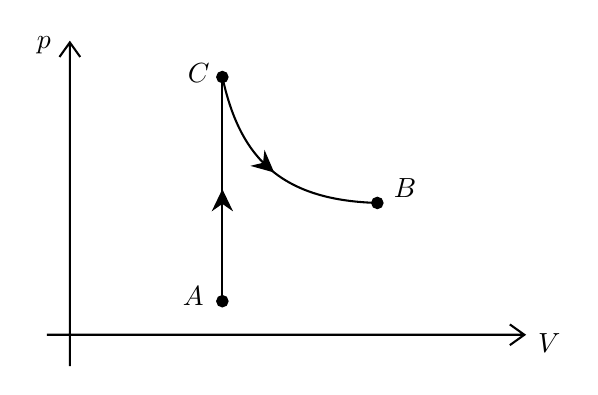
\begin{tikzpicture}[x=0.75pt,y=0.75pt,yscale=-1,xscale=1]
	%uncomment if require: \path (0,300); %set diagram left start at 0, and has height of 300

	%Shape: Axis 2D [id:dp26852410186154585] 
	\draw  (128.5,213.85) -- (358.5,213.85)(139.52,73) -- (139.52,229) (351.5,208.85) -- (358.5,213.85) -- (351.5,218.85) (134.52,80) -- (139.52,73) -- (144.52,80)  ;
	%Straight Lines [id:da33150538466512813] 
	\draw    (213,89.67) -- (213,197.67) ;
	\draw [shift={(213,143.67)}, rotate = 90] [fill={rgb, 255:red, 0; green, 0; blue, 0 }  ][line width=0.08]  [draw opacity=0] (10.72,-5.15) -- (0,0) -- (10.72,5.15) -- (7.12,0) -- cycle    ;
	%Curve Lines [id:da23260166306084673] 
	\draw    (213,89.67) .. controls (221,126.33) and (239,149) .. (287.67,150.33) ;
	\draw [shift={(237.96,135.66)}, rotate = 221.21] [fill={rgb, 255:red, 0; green, 0; blue, 0 }  ][line width=0.08]  [draw opacity=0] (10.72,-5.15) -- (0,0) -- (10.72,5.15) -- (7.12,0) -- cycle    ;
	%Shape: Circle [id:dp7685148264751998] 
	\draw  [fill={rgb, 255:red, 0; green, 0; blue, 0 }  ,fill opacity=1 ] (213,200.17) .. controls (211.62,200.17) and (210.5,199.05) .. (210.5,197.67) .. controls (210.5,196.29) and (211.62,195.17) .. (213,195.17) .. controls (214.38,195.17) and (215.5,196.28) .. (215.5,197.67) .. controls (215.5,199.05) and (214.38,200.17) .. (213,200.17) -- cycle ;
	%Shape: Circle [id:dp6135691859180823] 
	\draw  [fill={rgb, 255:red, 0; green, 0; blue, 0 }  ,fill opacity=1 ] (213,92.17) .. controls (211.62,92.17) and (210.5,91.05) .. (210.5,89.67) .. controls (210.5,88.29) and (211.62,87.17) .. (213,87.17) .. controls (214.38,87.17) and (215.5,88.28) .. (215.5,89.67) .. controls (215.5,91.05) and (214.38,92.17) .. (213,92.17) -- cycle ;
	%Shape: Circle [id:dp757889220486204] 
	\draw  [fill={rgb, 255:red, 0; green, 0; blue, 0 }  ,fill opacity=1 ] (287.67,152.83) .. controls (286.29,152.83) and (285.17,151.72) .. (285.17,150.33) .. controls (285.17,148.95) and (286.28,147.83) .. (287.67,147.83) .. controls (289.05,147.83) and (290.17,148.95) .. (290.17,150.33) .. controls (290.17,151.71) and (289.05,152.83) .. (287.67,152.83) -- cycle ;

	% Text Node
	\draw (127,74.5) node    {$p$};
	% Text Node
	\draw (370.5,218) node    {$V$};
	% Text Node
	\draw (301,143.17) node    {$B$};
	% Text Node
	\draw (199,195.17) node    {$A$};
	% Text Node
	\draw (201.67,87.83) node    {$C$};

	\end{tikzpicture}
\end{figure}
\FloatBarrier
Questo stato lo si chiama $C$. Poi si riscalda (o raffredda) il gas in maniera isocora, cioè a volume costante, fino ad arrivare ad $A$. Al contrario, quando si parte dallo stato iniziale $A$, si riscalda il gas fino allo stato $C$ a volume costante, e con una isoterma si arriva a $B$.
Si può quindi vedere la variazione dell'energia interna come:

\[
	\Delta U = U(B)-U(A) = [U(C)-U(A)] + [U(B)-U(C)]
\]

La seconda variazione di energia interna vale zero perché la temperatura in $B$ e in $C$ è la stessa. Quindi rimane soltanto da calcolare il primo termine. Da $A$ a $C$ non c'è lavoro compiuto dal gas perché non c'è variazione di pressione. Si calcola il calore scambiato sfruttando la definizione di calore specifico molare, con queste informazioni:

\[
	\Delta U_{A\to C} = Q_{\text{isocora} } - \underbrace{\mathcal{L}_{\text{isocora} }}_{=0} = nc_v(T_C-T_A  )
\]
$T_C$ è uguale a $T_B$ visto che la seconda trasformazione è isoterma. Si ottiene che la variazione di energia interna dallo stato iniziale $A$ allo stato finale $B$ è esprimibile come:

\[
	\Delta U = nc_v(T_B-T_A  )
\]

La variazione di energia interna per un gas perfetto sarà sempre la stessa. Questa espressione vale per qualunque trasformazione.

\paragraph{Lavoro in un'isoterma} Si immagini di far espandere il gas lungo una certa trasformazione isoterma. Si ha un recipiente contenente un certo numero di moli ad una certa pressione, volume e temperatura. Il contenitore è mantenuto a contatto con un serbatoio di calore la cui temperatura è sempre $T_0$ e anche se cede o assorbe calore non la varia. Sul pistone mobile è appoggiata una certa massa $m$, per cui il gas inizialmente deve essere alla stessa pressione che sta all'esterno. Essa è la pressione atmosferica più la pressione data dalla massa. Mantenendo il contatto con il serbatoio si rimuove la massa. Il gas si espande perché deve andare in equilibrio con la pressione esterna,  atmosferica.

\begin{figure}[htpb]
	\centering

	% Pattern Info
	 
	\tikzset{
	pattern size/.store in=\mcSize, 
	pattern size = 5pt,
	pattern thickness/.store in=\mcThickness, 
	pattern thickness = 0.3pt,
	pattern radius/.store in=\mcRadius, 
	pattern radius = 1pt}
	\makeatletter
	\pgfutil@ifundefined{pgf@pattern@name@_1xlpa3eg8}{
	\pgfdeclarepatternformonly[\mcThickness,\mcSize]{_1xlpa3eg8}
	{\pgfqpoint{0pt}{-\mcThickness}}
	{\pgfpoint{\mcSize}{\mcSize}}
	{\pgfpoint{\mcSize}{\mcSize}}
	{
	\pgfsetcolor{\tikz@pattern@color}
	\pgfsetlinewidth{\mcThickness}
	\pgfpathmoveto{\pgfqpoint{0pt}{\mcSize}}
	\pgfpathlineto{\pgfpoint{\mcSize+\mcThickness}{-\mcThickness}}
	\pgfusepath{stroke}
	}}
	\makeatother

	% Pattern Info
	 
	\tikzset{
	pattern size/.store in=\mcSize, 
	pattern size = 5pt,
	pattern thickness/.store in=\mcThickness, 
	pattern thickness = 0.3pt,
	pattern radius/.store in=\mcRadius, 
	pattern radius = 1pt}
	\makeatletter
	\pgfutil@ifundefined{pgf@pattern@name@_7ausj6b50}{
	\pgfdeclarepatternformonly[\mcThickness,\mcSize]{_7ausj6b50}
	{\pgfqpoint{0pt}{-\mcThickness}}
	{\pgfpoint{\mcSize}{\mcSize}}
	{\pgfpoint{\mcSize}{\mcSize}}
	{
	\pgfsetcolor{\tikz@pattern@color}
	\pgfsetlinewidth{\mcThickness}
	\pgfpathmoveto{\pgfqpoint{0pt}{\mcSize}}
	\pgfpathlineto{\pgfpoint{\mcSize+\mcThickness}{-\mcThickness}}
	\pgfusepath{stroke}
	}}
	\makeatother
	\tikzset{every picture/.style={line width=0.75pt}} %set default line width to 0.75pt        

	\begin{tikzpicture}[x=0.75pt,y=0.75pt,yscale=-1,xscale=1]
	%uncomment if require: \path (0,300); %set diagram left start at 0, and has height of 300

	%Straight Lines [id:da09277888142735424] 
	\draw    (130,100) -- (130,200) ;
	%Straight Lines [id:da4610100840831337] 
	\draw    (220,100) -- (220,200) ;
	%Straight Lines [id:da7210267727104362] 
	\draw    (130,200) -- (220,200) ;
	%Straight Lines [id:da2693208501217441] 
	\draw [line width=2.25]    (130,141) -- (220,141) ;
	%Shape: Circle [id:dp1542212791327302] 
	\draw  [draw opacity=0][fill={rgb, 255:red, 212; green, 212; blue, 212 }  ,fill opacity=1 ] (158.5,156.13) .. controls (158.5,151.64) and (162.14,148) .. (166.63,148) .. controls (171.11,148) and (174.75,151.64) .. (174.75,156.13) .. controls (174.75,160.61) and (171.11,164.25) .. (166.63,164.25) .. controls (162.14,164.25) and (158.5,160.61) .. (158.5,156.13) -- cycle ;
	%Shape: Circle [id:dp8517752557618017] 
	\draw  [draw opacity=0][fill={rgb, 255:red, 212; green, 212; blue, 212 }  ,fill opacity=1 ] (184,153.13) .. controls (184,148.64) and (187.64,145) .. (192.13,145) .. controls (196.61,145) and (200.25,148.64) .. (200.25,153.13) .. controls (200.25,157.61) and (196.61,161.25) .. (192.13,161.25) .. controls (187.64,161.25) and (184,157.61) .. (184,153.13) -- cycle ;
	%Shape: Circle [id:dp415834616408854] 
	\draw  [draw opacity=0][fill={rgb, 255:red, 212; green, 212; blue, 212 }  ,fill opacity=1 ] (140.5,167.63) .. controls (140.5,163.14) and (144.14,159.5) .. (148.63,159.5) .. controls (153.11,159.5) and (156.75,163.14) .. (156.75,167.63) .. controls (156.75,172.11) and (153.11,175.75) .. (148.63,175.75) .. controls (144.14,175.75) and (140.5,172.11) .. (140.5,167.63) -- cycle ;
	%Shape: Circle [id:dp9194075293630759] 
	\draw  [draw opacity=0][fill={rgb, 255:red, 212; green, 212; blue, 212 }  ,fill opacity=1 ] (174,170.63) .. controls (174,166.14) and (177.64,162.5) .. (182.13,162.5) .. controls (186.61,162.5) and (190.25,166.14) .. (190.25,170.63) .. controls (190.25,175.11) and (186.61,178.75) .. (182.13,178.75) .. controls (177.64,178.75) and (174,175.11) .. (174,170.63) -- cycle ;
	%Shape: Circle [id:dp5830961561003043] 
	\draw  [draw opacity=0][fill={rgb, 255:red, 212; green, 212; blue, 212 }  ,fill opacity=1 ] (139,187.63) .. controls (139,183.14) and (142.64,179.5) .. (147.13,179.5) .. controls (151.61,179.5) and (155.25,183.14) .. (155.25,187.63) .. controls (155.25,192.11) and (151.61,195.75) .. (147.13,195.75) .. controls (142.64,195.75) and (139,192.11) .. (139,187.63) -- cycle ;
	%Shape: Circle [id:dp17728094173428888] 
	\draw  [draw opacity=0][fill={rgb, 255:red, 212; green, 212; blue, 212 }  ,fill opacity=1 ] (199.5,164.63) .. controls (199.5,160.14) and (203.14,156.5) .. (207.63,156.5) .. controls (212.11,156.5) and (215.75,160.14) .. (215.75,164.63) .. controls (215.75,169.11) and (212.11,172.75) .. (207.63,172.75) .. controls (203.14,172.75) and (199.5,169.11) .. (199.5,164.63) -- cycle ;
	%Shape: Circle [id:dp6783241133698021] 
	\draw  [draw opacity=0][fill={rgb, 255:red, 212; green, 212; blue, 212 }  ,fill opacity=1 ] (159.5,187.63) .. controls (159.5,183.14) and (163.14,179.5) .. (167.63,179.5) .. controls (172.11,179.5) and (175.75,183.14) .. (175.75,187.63) .. controls (175.75,192.11) and (172.11,195.75) .. (167.63,195.75) .. controls (163.14,195.75) and (159.5,192.11) .. (159.5,187.63) -- cycle ;
	%Shape: Circle [id:dp8098719490652282] 
	\draw  [draw opacity=0][fill={rgb, 255:red, 212; green, 212; blue, 212 }  ,fill opacity=1 ] (191,185.13) .. controls (191,180.64) and (194.64,177) .. (199.13,177) .. controls (203.61,177) and (207.25,180.64) .. (207.25,185.13) .. controls (207.25,189.61) and (203.61,193.25) .. (199.13,193.25) .. controls (194.64,193.25) and (191,189.61) .. (191,185.13) -- cycle ;
	%Shape: Rectangle [id:dp04965632327927327] 
	\draw  [draw opacity=0][fill={rgb, 255:red, 74; green, 74; blue, 74 }  ,fill opacity=1 ] (161.5,124.5) -- (188.25,124.5) -- (188.25,139.5) -- (161.5,139.5) -- cycle ;
	%Rounded Rect [id:dp5179782246702531] 
	\draw  [pattern=_1xlpa3eg8,pattern size=6pt,pattern thickness=0.75pt,pattern radius=0pt, pattern color={rgb, 255:red, 155; green, 155; blue, 155}] (120.25,204) .. controls (120.25,201.79) and (122.04,200) .. (124.25,200) -- (226.75,200) .. controls (228.96,200) and (230.75,201.79) .. (230.75,204) -- (230.75,216) .. controls (230.75,218.21) and (228.96,220) .. (226.75,220) -- (124.25,220) .. controls (122.04,220) and (120.25,218.21) .. (120.25,216) -- cycle ;
	%Straight Lines [id:da5802141561376881] 
	\draw    (260,100) -- (260,200) ;
	%Straight Lines [id:da19175209152388706] 
	\draw    (350,100) -- (350,200) ;
	%Straight Lines [id:da12090357925191442] 
	\draw    (260,200) -- (350,200) ;
	%Straight Lines [id:da4269274783694801] 
	\draw [line width=2.25]    (260,107) -- (350,107) ;
	%Shape: Circle [id:dp831118661671322] 
	\draw  [draw opacity=0][fill={rgb, 255:red, 212; green, 212; blue, 212 }  ,fill opacity=1 ] (266.5,123.46) .. controls (266.5,118.97) and (270.14,115.33) .. (274.63,115.33) .. controls (279.11,115.33) and (282.75,118.97) .. (282.75,123.46) .. controls (282.75,127.95) and (279.11,131.58) .. (274.63,131.58) .. controls (270.14,131.58) and (266.5,127.95) .. (266.5,123.46) -- cycle ;
	%Shape: Circle [id:dp543457889317305] 
	\draw  [draw opacity=0][fill={rgb, 255:red, 212; green, 212; blue, 212 }  ,fill opacity=1 ] (298.33,124.79) .. controls (298.33,120.3) and (301.97,116.67) .. (306.46,116.67) .. controls (310.95,116.67) and (314.58,120.3) .. (314.58,124.79) .. controls (314.58,129.28) and (310.95,132.92) .. (306.46,132.92) .. controls (301.97,132.92) and (298.33,129.28) .. (298.33,124.79) -- cycle ;
	%Shape: Circle [id:dp7341469396289795] 
	\draw  [draw opacity=0][fill={rgb, 255:red, 212; green, 212; blue, 212 }  ,fill opacity=1 ] (280.5,150.96) .. controls (280.5,146.47) and (284.14,142.83) .. (288.63,142.83) .. controls (293.11,142.83) and (296.75,146.47) .. (296.75,150.96) .. controls (296.75,155.45) and (293.11,159.08) .. (288.63,159.08) .. controls (284.14,159.08) and (280.5,155.45) .. (280.5,150.96) -- cycle ;
	%Shape: Circle [id:dp3081150642569459] 
	\draw  [draw opacity=0][fill={rgb, 255:red, 212; green, 212; blue, 212 }  ,fill opacity=1 ] (322,135.29) .. controls (322,130.8) and (325.64,127.17) .. (330.13,127.17) .. controls (334.61,127.17) and (338.25,130.8) .. (338.25,135.29) .. controls (338.25,139.78) and (334.61,143.42) .. (330.13,143.42) .. controls (325.64,143.42) and (322,139.78) .. (322,135.29) -- cycle ;
	%Shape: Circle [id:dp8597573232998028] 
	\draw  [draw opacity=0][fill={rgb, 255:red, 212; green, 212; blue, 212 }  ,fill opacity=1 ] (269,187.63) .. controls (269,183.14) and (272.64,179.5) .. (277.13,179.5) .. controls (281.61,179.5) and (285.25,183.14) .. (285.25,187.63) .. controls (285.25,192.11) and (281.61,195.75) .. (277.13,195.75) .. controls (272.64,195.75) and (269,192.11) .. (269,187.63) -- cycle ;
	%Shape: Circle [id:dp25298104539020194] 
	\draw  [draw opacity=0][fill={rgb, 255:red, 212; green, 212; blue, 212 }  ,fill opacity=1 ] (291.5,172.63) .. controls (291.5,168.14) and (295.14,164.5) .. (299.62,164.5) .. controls (304.11,164.5) and (307.75,168.14) .. (307.75,172.63) .. controls (307.75,177.11) and (304.11,180.75) .. (299.62,180.75) .. controls (295.14,180.75) and (291.5,177.11) .. (291.5,172.63) -- cycle ;
	%Shape: Circle [id:dp21127649154398997] 
	\draw  [draw opacity=0][fill={rgb, 255:red, 212; green, 212; blue, 212 }  ,fill opacity=1 ] (316.83,158.96) .. controls (316.83,154.47) and (320.47,150.83) .. (324.96,150.83) .. controls (329.45,150.83) and (333.08,154.47) .. (333.08,158.96) .. controls (333.08,163.45) and (329.45,167.08) .. (324.96,167.08) .. controls (320.47,167.08) and (316.83,163.45) .. (316.83,158.96) -- cycle ;
	%Shape: Circle [id:dp37293066534985364] 
	\draw  [draw opacity=0][fill={rgb, 255:red, 212; green, 212; blue, 212 }  ,fill opacity=1 ] (321,185.13) .. controls (321,180.64) and (324.64,177) .. (329.13,177) .. controls (333.61,177) and (337.25,180.64) .. (337.25,185.13) .. controls (337.25,189.61) and (333.61,193.25) .. (329.13,193.25) .. controls (324.64,193.25) and (321,189.61) .. (321,185.13) -- cycle ;
	%Rounded Rect [id:dp8417795589498158] 
	\draw  [pattern=_7ausj6b50,pattern size=6pt,pattern thickness=0.75pt,pattern radius=0pt, pattern color={rgb, 255:red, 155; green, 155; blue, 155}] (250.25,204) .. controls (250.25,201.79) and (252.04,200) .. (254.25,200) -- (356.75,200) .. controls (358.96,200) and (360.75,201.79) .. (360.75,204) -- (360.75,216) .. controls (360.75,218.21) and (358.96,220) .. (356.75,220) -- (254.25,220) .. controls (252.04,220) and (250.25,218.21) .. (250.25,216) -- cycle ;

	% Text Node
	\draw (175,230) node   [align=left] {serbatoio};
	% Text Node
	\draw (305,230) node   [align=left] {serbatoio};

	\end{tikzpicture}
\end{figure}
\FloatBarrier
Il volume sarà cambiato, il numero di moli è lo stesso, la temperatura è sempre $T_0$. Conoscendo lo stato iniziale e finale, bisogna capire se il sistema scambia energia con l'ambiente esterno. Si applica il primo principio della termodinamica:

\[
	\Delta U = Q_{\text{isoterma} }- \mathcal{L}_{\text{isoterma} } \quad \Delta U = 0 \implies \underbrace{Q_{\text{isoterma} }}_{>0} = \underbrace{\mathcal{L}_{\text{isoterma} }}_{>0}
\]

L'energia interna del sistema non varia perché dipende solo dalla temperatura. Il calore scambiato deve essere pari al lavoro compiuto. Durante la trasformazione, per potersi espandere, il gas deve assorbire calore dal serbatoio e convertirlo in lavoro meccanico di espansione. Sul calcolo del lavoro si distinguono i casi a seconda che la trasformazione venga fatta in maniera reversibile o irreversibile, perché il calore assorbito sarà diverso.
Si supponga che la trasformazione venga fatta in maniera reversibile, per passaggi continui dallo stato di equilibrio. Il metodo è eliminare tutti gli attriti in modo che quando il pistone scorre verso l'alto non dissipa energia. Bisogna poi immaginare la massa $m$ come un sacchetto di sabbia, dal quale si toglie un granello alla volta. Se si fa avvenire la trasformazione molto lentamente, il gas si assesta in condizioni di equilibrio molto vicine. Questo è un modo per far avvenire la trasformazione in maniera quai statica.

\[
	\mathcal{L}_{\text{isoterma} }= \int\rho_{\text{gas} }dV = \int \frac{nRT_0 }{V}dV = nRT_0\,\log \left( \frac{V_f}{V_i} \right)
\]

La trasformazione irreversibile si ha quando si rimuove il blocco in un colpo. L'istante in cui inizia la trasformazione, è già quello in cui il blocco è rimosso. Non si può conoscere la pressione del gas negli stati intermedi, quindi si calcola il lavoro come l'opposto di quello compiuto sull'ambiente esterno. Dall'istante iniziale la pressione atmosferica subisce una compressione da parte del gas. Si può calcolare il lavoro del gas come quello subito dall'ambiente esterno:

\[
	\mathcal{L}_{\text{isoterma} } =\int \rho_{\text{gas} }dV = -\mathcal{L}_{est} = p_{est}\Delta V = p_{atm}\Delta V_{\text{gas} }    	
\]

\paragraph{Lavoro in una isocora} Si hanno $n$ moli di gas, in un recipiente rigido a contatto con un serbatoio termico. Si cambia serbatoio con uno a temperatura maggiore. Il gas piano piano va in equilibrio termico con esso. Il volume non sarà cambiato (nessun lavoro compiuto) ma ci si aspetta che la pressione lo sia. Il gas aumenta la sua energia interna grazie al fatto che assorbe calore dal serbatoio.

\[Q-\mathcal{L}=Q=\Delta U\]

Lo scambio energetico non dipende dal fatto che la trasformazione sia fatta in modo reversibile o irreversibile, perché non viene compiuto lavoro, quindi il calore scambiato sarà sempre lo stesso.

\paragraph{Lavoro in un'isobara} Si riscalda un gas a pressione costante. Esso si trova in equilibrio con la pressione esterna $p_0$ e con la temperatura del serbatoio. Si vede quali sono i contributi energetici lungo la trasformazione. Si può scrivere che:

\begin{align*}
	Q_{\text{isobara}} &= \Delta U + \mathcal{L}_{\text{isobara}} \\
		&= \Delta U + p_0\Delta V \\
		&= nc_v\Delta T + \underbrace{p_0\Delta V}_{=nR\Delta T} = n\Delta T\,c_p \tag*{(in un'isobara)} \\
		&= nc_v\Delta T + nR\Delta T = n\Delta T c_p \\
		& \qquad \implies \boxed{c_v + R = c_p  } \\
\end{align*}

Si ottiene una relazione che mostra come il calore specifico a pressione costante sarà sempre maggiore di quello a volume costante. Infatti a pressione costante il gas usa parte del calore per compiere lavoro.

Da tale relazione si ricava un significato energetico per la costante dei gas ideali $R$: essa rappresenta il lavoro che a pressione costante compie $1 mol$.

\[
	\boxed{c_v + R = c_p  }  \qquad \text{relazione di Mayer}
\]

\paragraph{Trasformazioni adiabatiche reversibili} Si ha un gas perfetto contenuto in un recipiente in cui tutte le pareti sono adiabatiche, non permettono passaggio di calore all'esterno. Il gas si trova alla pressione $p_0$ e alla temperatura $T_0$. Si dovrà immaginare di poter rimuovere un'ipotetica massa sopra il pistone molto lentamente. Alla fine si avrà che il gas è andato in equilibrio con la pressione atmosferica. Il volume e la temperatura saranno cambiati. Espandendosi si avrà una diminuzione della pressione e una variazione della temperatura. Tutte e tre le variabili termodinamiche cambiano (caratteristica tipica delle adiabatiche). La pressione finale è tale da bilanciare quella esterna. Rimangono quindi due variabili termodinamiche da calcolare. Una la dà l'equazione di stato. Manca ancora una relazione per ricavare la terza variabile, si sfrutta quindi il primo principio della termodinamica:

\[
	\Delta U = \underbrace{Q}_{=0} - \mathcal{L}
\]

A fronte di un lavoro di espansione positivo fatto dal gas, ci si deve aspettare una diminuzione dell'energia interna accumulata e quindi un raffreddamento del gas. Si scrive il primo principio della termodinamica in forma infinitesima:

\[
	dU = dQ - d\mathcal{L}  \implies dU + d\mathcal{L} = 0
\]

La variazione infinitesima di energia interna sarà quindi $n c_v dT$. Il lavoro fatto dal gas sarà $p\,dV$. Si potrà inserire la relazione che lega la pressione con le altre variabili.

\begin{align*}
	n c_v dT + n\overbrace{R}^{c_p-c_v}T \frac{dV}{V} &= 0 \\
	\frac{c_v dT}{T} + (c_p-c_v)\frac{dV}{V} &= 0 \tag*{dividendo per $nT$} \\
	\frac{dT}{T} + \left(\frac{c_p}{c_v}-1\right)\frac{dV}{V} &= 0 \tag*{dividendo per $c_v$}\\
	\frac{dT}{T} &= \left( 1-\frac{c_p }{c_v} \right) \frac{dV}{V} \\
	\frac{dT}{T} &= \left( 1- \gamma \right) \frac{dV}{V} \\
	\int_{T_0 }^T \frac{dT}{T} &= \int_{V_0 }^V \left( 1- \gamma \right) \frac{dV}{V} \tag*{integrando}\\
\end{align*}

\begin{align*}
	\log \frac{T}{T_0} &= (1-\gamma) \log \frac{V}{V_0} \\
	\log \frac{T}{T_0} &= \log \left(\frac{V_0}{V}\right)^{\gamma-1} \\
	\frac{T}{T_0} &= \left( \frac{V_0}{V} \right)^{\gamma -1} \\
	TV^{\gamma -1} &= T_0 V_0^{\gamma -1}
\end{align*}
È stata trovata una relazione tra le variabili termodinamiche durante il processo adiabatico reversibile.

\[
	\boxed{TV^{\gamma -1} = \text{costante}}
\]
È una relazione caratteristica delle adiabatiche reversibili. A partire da questa relazione inseriamo la pressione per trovare un legame di questa con il volume.

\[
	\frac{pV}{nR}V^{\gamma -1} = \frac{p_0 V_0}{nR}V_0^{\gamma -1} \implies pV^{\gamma }=p_0 V_0^{\gamma } \implies \boxed{pV^{\gamma} = \text{costante}}
\]

Questo vuole fondamentalmente dire che tale è l'espansione che subirà il gas quando lo si fa espandere lungo un'adiabatica reversibile. Nell'isoterma, il gas parte dalla posizione $p_0$ e dal volume $V_0$, si espande fino alla pressione finale, quella atmosferica, e arriva a un certo volume finale. Nell'adiabatica reversibile, il gas si espande per arrivare alla stessa pressione finale e si raffredda. 

\begin{figure}[htpb]
	\centering

	\tikzset{every picture/.style={line width=0.75pt}} %set default line width to 0.75pt        

	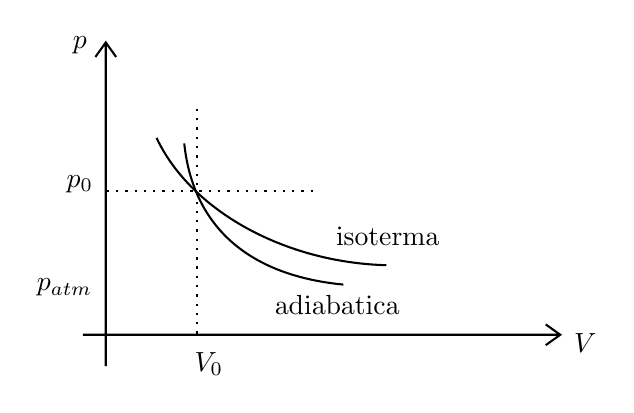
\begin{tikzpicture}[x=0.75pt,y=0.75pt,yscale=-1,xscale=1]
	%uncomment if require: \path (0,300); %set diagram left start at 0, and has height of 300

	%Shape: Axis 2D [id:dp27504680673319837] 
	\draw  (128.5,213.85) -- (358.5,213.85)(139.52,73) -- (139.52,229) (351.5,208.85) -- (358.5,213.85) -- (351.5,218.85) (134.52,80) -- (139.52,73) -- (144.52,80)  ;
	%Curve Lines [id:da9113262903740069] 
	\draw    (164,119) .. controls (180.67,154.33) and (226,179) .. (274.67,180.33) ;
	%Curve Lines [id:da8659384784035273] 
	\draw    (177.33,121.67) .. controls (181.33,159.67) and (206,185) .. (254,189.67) ;
	%Straight Lines [id:da5714540065534941] 
	\draw  [dash pattern={on 0.84pt off 2.51pt}]  (140,144.67) -- (239.33,144.67) ;
	%Straight Lines [id:da8284301291991147] 
	\draw  [dash pattern={on 0.84pt off 2.51pt}]  (183.67,213.33) -- (183.67,103) ;

	% Text Node
	\draw (127,74.5) node    {$p$};
	% Text Node
	\draw (370.5,218) node    {$V$};
	% Text Node
	\draw (127,141.17) node    {$p_{0}$};
	% Text Node
	\draw (119.67,191.17) node    {$p_{atm}$};
	% Text Node
	\draw (189.17,228) node    {$V_{0}$};
	% Text Node
	\draw (275.33,166.33) node   [align=left] {isoterma};
	% Text Node
	\draw (251,199.67) node   [align=left] {adiabatica};

	\end{tikzpicture}
\end{figure}
\FloatBarrier
Essa passa sicuramente sotto all'isoterma reversibile perché $\gamma$ è maggiore di $1$, infatti il gas si raffredda quindi questo stato finale deve essere sull'adiabatica più in basso.
Il lavoro adiabatico può essere calcolato facilmente come l'opposto della variazione dell'energia interna. Si può anche calcolarlo come area sottesa dalla curva anche se il procedimento è più complicato.
Nella pratica l'adiabaticità perfetta non esiste: tutte le sostanze con cui si realizzano pareti adiabatiche permettono un certo scambio di calore. Si ammette che possa essere adiabatica una trasformazione che avviene rapidamente, così che non ci sia tempo per scambi di calore apprezzabili.

\paragraph{Trasformazioni adiabatiche irreversibili} Se si realizza lo stesso processo in maniera irreversibile, togliendo ad esempio la massa che comprime il gas in un solo istante, non si potrà arrivare allo stesso volume $V$. Questo perché per trovare $pV^{\gamma}=\text{costante}$, è stato imposto che le variabili termodinamiche del gas in ogni punto soddisfino l'equazione di stato. Se il processo non lo si fa avvenire in maniera quasi statica non può valere la relazione trovata. Se si arriva a un volume finale diverso, il lavoro fatto dal gas durante il processo irreversibile adiabatico è diverso da quello compiuto durante il processo reversibile adiabatico.
Si può comunque affermare che la variazione di energia interna sarà pari e opposta al lavoro fatto dal gas, ma si dovrà introdurre un'altra relazione per trovare entrambe le variabili incognite. Un'idea è quella di scrivere il lavoro come l'opposto di quello subito dall'ambiente esterno. Esso sarà dato da: $nc_v\Delta T = - p_{\text{fin}}\Delta V$.


\paragraph{}\hspace{-1em}Si noti che tutte le trasformazioni reversibili viste possono essere scritte come:

\[
	pV^x=\text{costante} \left\{ \begin{array}{l}
	 	x = 0 \quad \text{isobara}  \\
	 	x = 1 \quad \text{isoterma}  \\
	 	x = \frac{c_p }{c_v } \quad \text{adiabatica}  \\
	 	x \to +\infty  \quad \text{isocora} \quad (p^{1/x}V=\text{costante}) \\
	\end{array} \right.
\]

Più in generale,  qualunque trasformazione \emph{reversibile} segue la legge:

\[
	\boxed{ pV^x=\text{cost}} \quad \text{dove }x=\frac{c_p-c_x  }{c_v-c_x  }
\]

e prende il nome di \textbf{politropica}. La dimostrazione si opera sfruttando il primo principio della termodinamica in modo molto simile a quello che ha portato a trovare l'equazione di una adiabatica reversibile. L'unica differenza sta nel fatto che $\delta Q$ non è uguale a $0$ ma sarà il calore scambiato con un certo calore specifico $c_x$.

\section{Macchine termodinamiche}

\subsection{Definizione e generalità}

Uno dei motivi per cui è nata la termodinamica è quello di realizzare macchine termiche, ossia dispositivi realizzanti processi che permettono di trasformare un'energia termica in lavoro meccanico. Un esempio semplice può essere l'espansione isoterma di un gas contenuto in un recipiente chiuso da un pistone e a contatto con un serbatoio. Essa avviene senza accumulo di energia interna: il calore fornito dal serbatoio si trasforma in lavoro meccanico. In tal caso il pistone si solleva una volta sola ma in genere si vuole che il lavoro meccanico venga ripetuto più volte. Questo significa che non basta realizzare la trasformazione una sola volta. Si mantiene sempre tutto a contatto con il serbatoio, e una volta che il pistone si è espanso si rimette la massa sopra facendo comprimere il sistema. In tal modo, il lavoro ottenuto passando da $A$ a $B$ lo si deve rifornire completamente tornando indietro, al netto non si è ottenuto nulla. Per realizzare un processo che al netto dia lavoro positivo, bisogna passare su una isoterma più bassa in modo tale che il lavoro tornando indietro sia meno intenso. Per fare ciò si segue in andata un tratto a pressione più alta di quello in cui avviene la compressione del gas. Questo è proprio un ciclo termodinamico caratteristico di una macchina termica.

\begin{figure}[htpb]
	\centering

	\tikzset{every picture/.style={line width=0.75pt}} %set default line width to 0.75pt        

	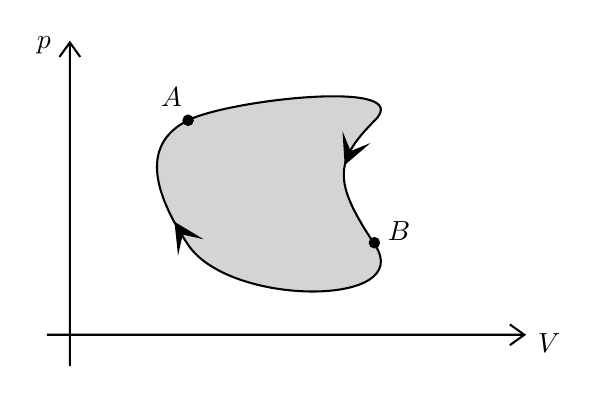
\begin{tikzpicture}[x=0.75pt,y=0.75pt,yscale=-1,xscale=1]
	%uncomment if require: \path (0,300); %set diagram left start at 0, and has height of 300

	%Shape: Polygon Curved [id:ds23043235146641394] 
	\draw  [fill={rgb, 255:red, 212; green, 212; blue, 212 }  ,fill opacity=1 ] (196.5,110.5) .. controls (216.5,100.5) and (306.5,90.5) .. (286.5,110.5) .. controls (266.5,130.5) and (266.5,140.5) .. (286.5,170.5) .. controls (306.5,200.5) and (216.5,200.5) .. (196.5,170.5) .. controls (176.5,140.5) and (176.5,120.5) .. (196.5,110.5) -- cycle ;
	%Shape: Axis 2D [id:dp7762746332730381] 
	\draw  (128.5,213.85) -- (358.5,213.85)(139.52,73) -- (139.52,229) (351.5,208.85) -- (358.5,213.85) -- (351.5,218.85) (134.52,80) -- (139.52,73) -- (144.52,80)  ;
	%Shape: Circle [id:dp27074858222439246] 
	\draw  [fill={rgb, 255:red, 0; green, 0; blue, 0 }  ,fill opacity=1 ] (194.25,110.5) .. controls (194.25,109.26) and (195.26,108.25) .. (196.5,108.25) .. controls (197.74,108.25) and (198.75,109.26) .. (198.75,110.5) .. controls (198.75,111.74) and (197.74,112.75) .. (196.5,112.75) .. controls (195.26,112.75) and (194.25,111.74) .. (194.25,110.5) -- cycle ;
	%Shape: Circle [id:dp6385622176143919] 
	\draw  [fill={rgb, 255:red, 0; green, 0; blue, 0 }  ,fill opacity=1 ] (284,169.5) .. controls (284,168.26) and (285.01,167.25) .. (286.25,167.25) .. controls (287.49,167.25) and (288.5,168.26) .. (288.5,169.5) .. controls (288.5,170.74) and (287.49,171.75) .. (286.25,171.75) .. controls (285.01,171.75) and (284,170.74) .. (284,169.5) -- cycle ;
	\draw  [fill={rgb, 255:red, 0; green, 0; blue, 0 }  ,fill opacity=1 ] (281.71,123.07) -- (272.36,131.07) -- (271.57,118.79) -- (274.5,126) -- cycle ;
	\draw  [fill={rgb, 255:red, 0; green, 0; blue, 0 }  ,fill opacity=1 ] (191.82,172.6) -- (190.54,160.36) -- (201.1,166.68) -- (193.5,165) -- cycle ;

	% Text Node
	\draw (127,74.5) node    {$p$};
	% Text Node
	\draw (370.5,218) node    {$V$};
	% Text Node
	\draw (188.5,99.17) node    {$A$};
	% Text Node
	\draw (298.17,163.67) node    {$B$};

	\end{tikzpicture}
\end{figure}
\FloatBarrier
Per un ciclo termodinamico si può sempre scrivere che:

\begin{gather*}
	\Delta U_{\text{ciclo} } = Q_{\text{ciclo} } - \mathcal{L}_{\text{ciclo} }=0 \\
	Q_{\text{ciclo} } = \mathcal{L}_{\text{ciclo} } > 0
\end{gather*}

La somma di tutti i calori scambiati durante il ciclo dà luogo al lavoro netto compiuto durante il ciclo. Il lavoro totale in un ciclo termodinamico reversibile è allora l'area racchiusa da esso.

Si può osservare sperimentalmente che non è mai possibile realizzare un processo che comporta come unico risultato la trasformazione di tutto il calore fornito in lavoro. Una parte di calore fornito sarà sempre ceduta all'ambiente circostante o ad un serbatoio a temperatura più bassa.

\begin{figure}[htpb]
	\centering

	\tikzset{every picture/.style={line width=0.75pt}} %set default line width to 0.75pt        

	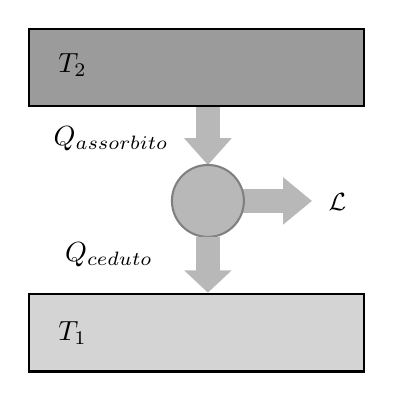
\begin{tikzpicture}[x=0.75pt,y=0.75pt,yscale=-1,xscale=1]
	%uncomment if require: \path (0,300); %set diagram left start at 0, and has height of 300

	%Right Arrow [id:dp038945600763613086] 
	\draw  [draw opacity=0][fill={rgb, 255:red, 184; green, 184; blue, 184 }  ,fill opacity=1 ] (175.06,108.44) -- (175.06,127.76) -- (180.8,127.76) -- (169.33,140.64) -- (157.87,127.76) -- (163.6,127.76) -- (163.6,108.44) -- cycle ;
	%Right Arrow [id:dp736310905270898] 
	\draw  [draw opacity=0][fill={rgb, 255:red, 184; green, 184; blue, 184 }  ,fill opacity=1 ] (184.67,152.24) -- (205.52,152.24) -- (205.52,146.51) -- (219.42,157.97) -- (205.52,169.44) -- (205.52,163.7) -- (184.67,163.7) -- cycle ;
	%Shape: Rectangle [id:dp49095902226996646] 
	\draw  [fill={rgb, 255:red, 155; green, 155; blue, 155 }  ,fill opacity=1 ] (83,75) -- (244.5,75) -- (244.5,112.27) -- (83,112.27) -- cycle ;
	%Shape: Rectangle [id:dp7012565668343214] 
	\draw  [fill={rgb, 255:red, 212; green, 212; blue, 212 }  ,fill opacity=1 ] (83,202.9) -- (244.5,202.9) -- (244.5,240.17) -- (83,240.17) -- cycle ;
	%Shape: Ellipse [id:dp5766499478882205] 
	\draw  [color={rgb, 255:red, 128; green, 128; blue, 128 }  ,draw opacity=1 ][fill={rgb, 255:red, 184; green, 184; blue, 184 }  ,fill opacity=1 ] (152,157.97) .. controls (152,148.4) and (159.76,140.64) .. (169.33,140.64) .. controls (178.91,140.64) and (186.67,148.4) .. (186.67,157.97) .. controls (186.67,167.55) and (178.91,175.31) .. (169.33,175.31) .. controls (159.76,175.31) and (152,167.55) .. (152,157.97) -- cycle ;
	%Right Arrow [id:dp6830856272799466] 
	\draw  [draw opacity=0][fill={rgb, 255:red, 184; green, 184; blue, 184 }  ,fill opacity=1 ] (175.06,175.31) -- (175.06,191.41) -- (180.8,191.41) -- (169.33,202.15) -- (157.87,191.41) -- (163.6,191.41) -- (163.6,175.31) -- cycle ;

	% Text Node
	\draw (122.67,128.17) node    {$Q_{\text{assorbito}}$};
	% Text Node
	\draw (121.67,183.83) node    {$Q_{\text{ceduto}}$};
	% Text Node
	\draw (104.12,92.39) node    {$T_{2}$};
	% Text Node
	\draw (104.12,221.53) node    {$T_{1}$};
	% Text Node
	\draw (231.8,158.27) node  [font=\small]  {$\mathcal{L}$};

	\end{tikzpicture}
\end{figure}
\FloatBarrier
È importante quindi che la frazione di calore trasformata in lavoro sia grande. Questo porta alla definizione di \textbf{rendimento} di una macchina termica, dato dal rapporto fra ciò che si ottiene e ciò che bisogna fornire per ottenerlo.

\begin{gather*}
	\eta = \text{rendimento} = \frac{\mathcal{L} }{Q_{\text{assorbito} } } > 0 \qquad 0 < \eta < 1 \quad \text{perché} \quad \mathcal{L} < Q_{\text{ass} } \\
	\underbrace{Q_{\text{ass}}}_{>0} + \underbrace{Q_{\text{ced}}}_{<0} = \mathcal{L} \quad \text{ossia} \quad Q_{\text{ass}} - |Q_{\text{ced}}| = \mathcal{L} \\
	\eta = \frac{Q_{\text{ass}} - |Q_{\text{ced}}|}{Q_{\text{ass}}} = 1 - \frac{|Q_{\text{ced}}|}{Q_{\text{ass}}}
\end{gather*}

Quest'ultimo modo di esprimere il rendimento, mette in evidenza che se non ci fosse calore ceduto (cosa irrealizzabile nella pratica), il rendimento sarebbe pari a $1$ e tutto il calore sarebbe trasformato in lavoro.

\subsection{Il ciclo di Carnot}

L'esempio concreto di macchina termica più importante che esiste è quella realizzabile facendo eseguire al sistema termodinamico un ciclo detto ciclo di Carnot.

\begin{figure}[htpb]
	\centering

	\tikzset{every picture/.style={line width=0.75pt}} %set default line width to 0.75pt        

	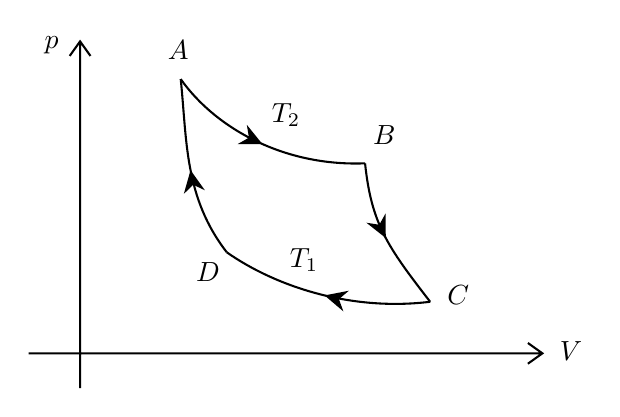
\begin{tikzpicture}[x=0.75pt,y=0.75pt,yscale=-1,xscale=1]
	%uncomment if require: \path (0,300); %set diagram left start at 0, and has height of 300

	%Shape: Axis 2D [id:dp48720272776316453] 
	\draw  (70,222.3) -- (317.5,222.3)(94.75,72) -- (94.75,239) (310.5,217.3) -- (317.5,222.3) -- (310.5,227.3) (89.75,79) -- (94.75,72) -- (99.75,79)  ;
	%Curve Lines [id:da6308193749582969] 
	\draw    (143.23,90.17) .. controls (160.08,113.9) and (193,132.28) .. (232.05,130.75) ;
	\draw [shift={(182.55,121.43)}, rotate = 205.42000000000002] [fill={rgb, 255:red, 0; green, 0; blue, 0 }  ][line width=0.08]  [draw opacity=0] (10.72,-5.15) -- (0,0) -- (10.72,5.15) -- (7.12,0) -- cycle    ;
	%Curve Lines [id:da6684877234044795] 
	\draw    (165.44,173.62) .. controls (188.4,189.7) and (224.64,202.2) .. (263.42,197.45) ;
	\draw [shift={(212.56,194.39)}, rotate = 14.74] [fill={rgb, 255:red, 0; green, 0; blue, 0 }  ][line width=0.08]  [draw opacity=0] (10.72,-5.15) -- (0,0) -- (10.72,5.15) -- (7.12,0) -- cycle    ;
	%Curve Lines [id:da4255798805877631] 
	\draw    (143.23,90.17) .. controls (146.29,119.26) and (144.76,146.92) .. (165.44,173.62) ;
	\draw [shift={(147.97,134.04)}, rotate = 80.14] [fill={rgb, 255:red, 0; green, 0; blue, 0 }  ][line width=0.08]  [draw opacity=0] (10.72,-5.15) -- (0,0) -- (10.72,5.15) -- (7.12,0) -- cycle    ;
	%Curve Lines [id:da2405649855739509] 
	\draw    (232.05,130.75) .. controls (235.11,159.84) and (242.75,170.75) .. (263.42,197.45) ;
	\draw [shift={(242.03,166.74)}, rotate = 244] [fill={rgb, 255:red, 0; green, 0; blue, 0 }  ][line width=0.08]  [draw opacity=0] (10.72,-5.15) -- (0,0) -- (10.72,5.15) -- (7.12,0) -- cycle    ;

	% Text Node
	\draw (81,74) node    {$p$};
	% Text Node
	\draw (331.33,221.33) node    {$V$};
	% Text Node
	\draw (142,76) node    {$A$};
	% Text Node
	\draw (241.33,117.33) node    {$B$};
	% Text Node
	\draw (277,194.33) node    {$C$};
	% Text Node
	\draw (156.33,183) node    {$D$};
	% Text Node
	\draw (202.67,177.33) node    {$T_{1}$};
	% Text Node
	\draw (194,107.33) node    {$T_{2}$};

	\end{tikzpicture}
\end{figure}
\FloatBarrier
Esso è costituito da:

\begin{itemize}
	\item Una espansione isoterma alla temperatura $T_2$ in cui il gas è a contatto con un serbatoio caldo. Esso espandendosi assorbe calore dal serbatoio e lo trasforma in lavoro ($AB$).
	\item Per abbassare la pressione si effettua un raffreddamento adiabatico ($BC$): si fa espandere il gas in maniera adiabatica reversibile.
	\item Poi si fa comprimere il gas in maniera isoterma, ma ad una temperatura più bassa di quella di partenza, perché esso si è raffreddato passando da $B$ a $C$. Il lavoro subito per questo sarà minore di quello compiuto nella fase di espansione ($CD$).
	\item Si esegue poi un riscaldamento adiabatico reversibile ($DA$).
\end{itemize}

Per calcolare il rendimento della macchina di Carnot, si mettono in evidenza le trasformazioni in cui c'è passaggio di calore con l'esterno (le due isoterme).
Si trova il calore assorbito:

\begin{align*}
	A\to B:\quad Q_{AB,\text{isoterma} } = \mathcal{L}_{AB} = \int p_{gas}dV &= \int_{V_A }^{V_B } \frac{nRT_2 }{V}dV \\
	&= nRT_2\log \left( \frac{V_B }{V_A } \right)
\end{align*}

E il calore ceduto:

\begin{gather*}
	C\to D:\quad Q_{CD,\text{isoterma}} = \mathcal{L}_{\text{isoterma} } = nRT_1\log \left( \frac{V_D }{V_C } \right) \\
	\eta = 1-\frac{|Q_{\text{ced} } |}{Q_{\text{ass} } } = 1 - \frac{nRT_1\log (V_c/V_D  ) }{nRT_2\log (V_B/V_A) }
\end{gather*}

Si aggiunge la relazione caratteristica che lega gli stati tra un'adiabatica reversibile.

\begin{gather*}
	B\to C:\quad TV^{\gamma -1}=\text{costante} \qquad T_2 V_B^{\gamma -1}=T_1 V_C^{\gamma -1} \\
	D\to A:\quad T_2 V_A^{\gamma -1} = T_1 V_D^{\gamma -1} \\
	\left( \frac{V_B }{V_A } \right)^{\gamma -1} = \left( \frac{V_C }{V_D } \right)^{\gamma -1} \implies \frac{V_B }{V_A }=\frac{V_C }{V_D } \implies \boxed{\eta = 1-\frac{T_1 }{T_2 }}
\end{gather*}

Si vede che il rendimento della macchina di Carnot dipende solo dalla temperatura dei due serbatoi. Sfruttando il primo principio della termodinamica, cioè il fatto che nella macchina termica si segue un ciclo termodinamico, si può affermare che il lavoro fatto è pari alla somma dei calori scambiati con l'ambiente circostante.

\section{Macchine frigorifere}

La termodinamica nasce anche per realizzare una seconda tipologia di macchine, che sono le macchine frigorifere. Si vuole mantenere l'ambiente all'interno del frigorifero ad una temperatura bassa $T_1$ e evitare che tenda a termalizzare con l'ambiente circostante. Si vuole invertire il processo secondo cui il calore passa dal corpo più caldo al corpo più freddo, fare in modo che avvenga il contrario. Non si tratta di un processo spontaneo, ecco perché per realizzarlo la macchina sfrutta il lavoro fornito dall'esterno.

\begin{figure}[htpb]
	\centering

	\tikzset{every picture/.style={line width=0.75pt}} %set default line width to 0.75pt        

	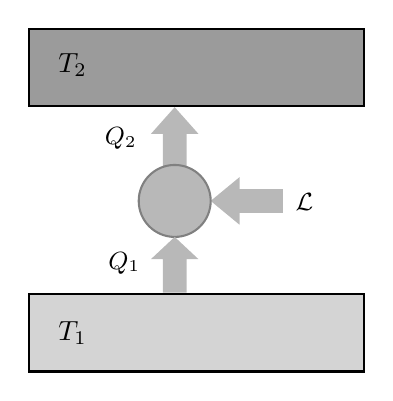
\begin{tikzpicture}[x=0.75pt,y=0.75pt,yscale=-1,xscale=1]
	%uncomment if require: \path (0,300); %set diagram left start at 0, and has height of 300

	%Right Arrow [id:dp6348625548042963] 
	\draw  [draw opacity=0][fill={rgb, 255:red, 184; green, 184; blue, 184 }  ,fill opacity=1 ] (222.6,154) -- (222.6,134.68) -- (216.87,134.68) -- (228.33,121.8) -- (239.8,134.68) -- (234.06,134.68) -- (234.06,154) -- cycle ;
	%Right Arrow [id:dp959084374703087] 
	\draw  [draw opacity=0][fill={rgb, 255:red, 184; green, 184; blue, 184 }  ,fill opacity=1 ] (280.42,172.7) -- (259.57,172.7) -- (259.57,178.44) -- (245.67,166.97) -- (259.57,155.51) -- (259.57,161.24) -- (280.42,161.24) -- cycle ;
	%Shape: Rectangle [id:dp8069606542485774] 
	\draw  [fill={rgb, 255:red, 155; green, 155; blue, 155 }  ,fill opacity=1 ] (158,84) -- (319.5,84) -- (319.5,121.27) -- (158,121.27) -- cycle ;
	%Shape: Rectangle [id:dp04641463651885647] 
	\draw  [fill={rgb, 255:red, 212; green, 212; blue, 212 }  ,fill opacity=1 ] (158,211.9) -- (319.5,211.9) -- (319.5,249.17) -- (158,249.17) -- cycle ;
	%Shape: Ellipse [id:dp8578905893334057] 
	\draw  [color={rgb, 255:red, 128; green, 128; blue, 128 }  ,draw opacity=1 ][fill={rgb, 255:red, 184; green, 184; blue, 184 }  ,fill opacity=1 ] (211,166.97) .. controls (211,157.4) and (218.76,149.64) .. (228.33,149.64) .. controls (237.91,149.64) and (245.67,157.4) .. (245.67,166.97) .. controls (245.67,176.55) and (237.91,184.31) .. (228.33,184.31) .. controls (218.76,184.31) and (211,176.55) .. (211,166.97) -- cycle ;
	%Right Arrow [id:dp9889661271891552] 
	\draw  [draw opacity=0][fill={rgb, 255:red, 184; green, 184; blue, 184 }  ,fill opacity=1 ] (222.6,211.15) -- (222.6,195.04) -- (216.87,195.04) -- (228.33,184.31) -- (239.8,195.04) -- (234.06,195.04) -- (234.06,211.15) -- cycle ;

	% Text Node
	\draw (179.12,101.39) node    {$T_{2}$};
	% Text Node
	\draw (179.12,230.53) node    {$T_{1}$};
	% Text Node
	\draw (202.37,137.03) node  [font=\small]  {$Q_{2}$};
	% Text Node
	\draw (204,196.87) node  [font=\small]  {$Q_{1}$};
	% Text Node
	\draw (290.8,167.27) node  [font=\small]  {$\mathcal{L}$};

	\end{tikzpicture}
\end{figure}
\FloatBarrier
Da un punto di vista pratico, per valutare la bontà di un frigorifero, si introduce un parametro di bontà che prende il nome di \textbf{efficienza frigorifera} o coefficiente di prestazione $\varepsilon$. Esso è il rapporto fra ciò che si vuole massimizzare, a scapito di ciò che si vuole fornire, il lavoro.

\[
	\varepsilon = \frac{Q_1 }{|\mathcal{L} |} < \infty
\]
È un lavoro fatto sul gas, quindi negativo: per avere un parametro positivo se ne utilizza allora il modulo.
Il processo non potrebbe mai avvenire senza immissione di lavoro, il denominatore non sarà mai zero, quindi l'efficienza non tenderà mai all'infinito. La si riscrive solo in termini di calori scambiati sfruttando il primo principio della termodinamica. Il ciclo termodinamico, visto che ci si aspetta un lavoro negativo, dovrà essere percorso in verso antiorario.
Si prende come esempio la macchina di Carnot, che si fa funzionare non come macchina termica ma come macchina frigorifera e quindi percorrendo il ciclo prima illustrato, ma in senso opposto.
Il gas per attuare questo processo deve ricevere un lavoro dall'ambiente circostante. Esso è rappresentato dall'area del ciclo, che in questo caso è negativa. Nella fase di espansione infatti viene compiuto un lavoro positivo ma nella fase di compressione il lavoro, che è negativo, è in modulo maggiore.
Poiché viene eseguito un ciclo, la somma dei calori scambiati è pari alla somma del lavoro fornito. La quantità $Q_1 - \abs{(Q_2)}$ è negativa. Si ha più calore ceduto all'ambiente cucina di quello che assorbito.

\[
	\Delta U_{\text{ciclo} } = Q - \mathcal{L}  = 0 \implies Q_1-|Q_2| = -|\mathcal{L}| < 0 \implies Q_1 < |Q_2|
\]

Andando a sostituire nell'espressione dell'efficienza frigorifera:

\[
	\varepsilon = \frac{Q_1 }{|Q_2| - Q_1 }
\]

Questa quantità è positiva e c'è sempre, non accadrà mai che tutto $Q_1$ diventi $Q_2$. Se si calcola il rendimento della particolare macchina frigorifera reversibile di Carnot (percorsa nell'altro senso) disegnata a lato, costituita da due isoterme e da due adiabatiche, si trova che:

\begin{align*}
	\varepsilon_{\text{Carnot} } &= \frac{Q_1 }{|Q_2| - |Q_1|} \\
	&= \frac{nRT_1\log (V_c/V_D  ) }{nRT_2\log (V_B/V_A) - nRT_1\log (V_C/V_D)} \\
	&=\frac{T_1 }{T_2-T_1  }
\end{align*}

Per questa particolare macchina termica frigorifera, il rendimento non dipende dal gas o dal numero di moli. Nel risultato del rendimento non compare $n$. Si è definito cosa sono una macchina termica e una macchina frigorifera. Esistono tanti esempi di macchine termiche e frigorifere che possono essere percorse con tanti tipi di cicli.

\paragraph{Ciclo di Stirling} È costituito da due isoterme e due isocore reversibili.

\begin{figure}[htpb]
	\centering

	\tikzset{every picture/.style={line width=0.75pt}} %set default line width to 0.75pt        

	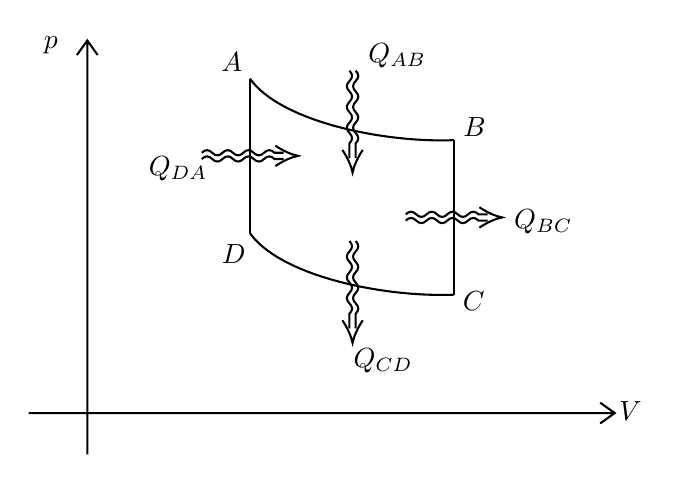
\begin{tikzpicture}[x=0.75pt,y=0.75pt,yscale=-1,xscale=1]
	%uncomment if require: \path (0,300); %set diagram left start at 0, and has height of 300

	%Shape: Axis 2D [id:dp09005657817363133] 
	\draw  (70,219.06) -- (352.33,219.06)(98.23,39.56) -- (98.23,239) (345.33,214.06) -- (352.33,219.06) -- (345.33,224.06) (93.23,46.56) -- (98.23,39.56) -- (103.23,46.56)  ;
	%Curve Lines [id:da25665381324207437] 
	\draw    (176.57,57.92) .. controls (191.27,78.63) and (240.8,88.92) .. (274.87,87.58) ;
	%Straight Lines [id:da9344352155729672] 
	\draw    (176.57,57.92) -- (176.57,132.37) ;
	%Curve Lines [id:da17826742079624203] 
	\draw    (176.57,132.37) .. controls (191.27,153.08) and (240.8,163.37) .. (274.87,162.03) ;
	%Straight Lines [id:da9751411952155511] 
	\draw    (274.87,87.58) -- (274.87,162.03) ;
	%Straight Lines [id:da019457556764712836] 
	\draw    (227.53,54.11) .. controls (229.2,55.78) and (229.2,57.44) .. (227.53,59.11) .. controls (225.86,60.78) and (225.86,62.44) .. (227.53,64.11) .. controls (229.2,65.78) and (229.2,67.44) .. (227.53,69.11) .. controls (225.86,70.78) and (225.86,72.44) .. (227.53,74.11) .. controls (229.2,75.78) and (229.2,77.44) .. (227.53,79.11) .. controls (225.86,80.78) and (225.86,82.44) .. (227.53,84.11) .. controls (229.2,85.78) and (229.2,87.44) .. (227.53,89.11) -- (227.53,93.22) -- (227.53,96.22)(224.53,54.11) .. controls (226.2,55.78) and (226.2,57.44) .. (224.53,59.11) .. controls (222.86,60.78) and (222.86,62.44) .. (224.53,64.11) .. controls (226.2,65.78) and (226.2,67.44) .. (224.53,69.11) .. controls (222.86,70.78) and (222.86,72.44) .. (224.53,74.11) .. controls (226.2,75.78) and (226.2,77.44) .. (224.53,79.11) .. controls (222.86,80.78) and (222.86,82.44) .. (224.53,84.11) .. controls (226.2,85.78) and (226.2,87.44) .. (224.53,89.11) -- (224.53,93.22) -- (224.53,96.22) ;
	\draw [shift={(226.03,103.22)}, rotate = 270] [color={rgb, 255:red, 0; green, 0; blue, 0 }  ][line width=0.75]    (10.93,-4.9) .. controls (6.95,-2.3) and (3.31,-0.67) .. (0,0) .. controls (3.31,0.67) and (6.95,2.3) .. (10.93,4.9)   ;
	%Straight Lines [id:da37819583599228856] 
	\draw    (227.53,136.2) .. controls (229.2,137.87) and (229.2,139.53) .. (227.53,141.2) .. controls (225.86,142.87) and (225.86,144.53) .. (227.53,146.2) .. controls (229.2,147.87) and (229.2,149.53) .. (227.53,151.2) .. controls (225.86,152.87) and (225.86,154.53) .. (227.53,156.2) .. controls (229.2,157.87) and (229.2,159.53) .. (227.53,161.2) .. controls (225.86,162.87) and (225.86,164.53) .. (227.53,166.2) .. controls (229.2,167.87) and (229.2,169.53) .. (227.53,171.2) -- (227.53,175.3) -- (227.53,178.3)(224.53,136.2) .. controls (226.2,137.87) and (226.2,139.53) .. (224.53,141.2) .. controls (222.86,142.87) and (222.86,144.53) .. (224.53,146.2) .. controls (226.2,147.87) and (226.2,149.53) .. (224.53,151.2) .. controls (222.86,152.87) and (222.86,154.53) .. (224.53,156.2) .. controls (226.2,157.87) and (226.2,159.53) .. (224.53,161.2) .. controls (222.86,162.87) and (222.86,164.53) .. (224.53,166.2) .. controls (226.2,167.87) and (226.2,169.53) .. (224.53,171.2) -- (224.53,175.3) -- (224.53,178.3) ;
	\draw [shift={(226.03,185.3)}, rotate = 270] [color={rgb, 255:red, 0; green, 0; blue, 0 }  ][line width=0.75]    (10.93,-4.9) .. controls (6.95,-2.3) and (3.31,-0.67) .. (0,0) .. controls (3.31,0.67) and (6.95,2.3) .. (10.93,4.9)   ;
	%Straight Lines [id:da5937334242417012] 
	\draw    (251.69,123.31) .. controls (253.36,121.64) and (255.02,121.64) .. (256.69,123.31) .. controls (258.36,124.98) and (260.02,124.98) .. (261.69,123.31) .. controls (263.36,121.64) and (265.02,121.64) .. (266.69,123.31) .. controls (268.36,124.98) and (270.02,124.98) .. (271.69,123.31) .. controls (273.36,121.64) and (275.02,121.64) .. (276.69,123.31) .. controls (278.36,124.98) and (280.02,124.98) .. (281.69,123.31) .. controls (283.36,121.64) and (285.02,121.64) .. (286.69,123.31) -- (288.05,123.31) -- (291.05,123.31)(251.69,126.31) .. controls (253.36,124.64) and (255.02,124.64) .. (256.69,126.31) .. controls (258.36,127.98) and (260.02,127.98) .. (261.69,126.31) .. controls (263.36,124.64) and (265.02,124.64) .. (266.69,126.31) .. controls (268.36,127.98) and (270.02,127.98) .. (271.69,126.31) .. controls (273.36,124.64) and (275.02,124.64) .. (276.69,126.31) .. controls (278.36,127.98) and (280.02,127.98) .. (281.69,126.31) .. controls (283.36,124.64) and (285.02,124.64) .. (286.69,126.31) -- (288.05,126.31) -- (291.05,126.31) ;
	\draw [shift={(298.05,124.81)}, rotate = 180] [color={rgb, 255:red, 0; green, 0; blue, 0 }  ][line width=0.75]    (10.93,-4.9) .. controls (6.95,-2.3) and (3.31,-0.67) .. (0,0) .. controls (3.31,0.67) and (6.95,2.3) .. (10.93,4.9)   ;
	%Straight Lines [id:da5637070421962109] 
	\draw    (153.39,93.65) .. controls (155.06,91.98) and (156.72,91.98) .. (158.39,93.65) .. controls (160.06,95.32) and (161.72,95.32) .. (163.39,93.65) .. controls (165.06,91.98) and (166.72,91.98) .. (168.39,93.65) .. controls (170.06,95.32) and (171.72,95.32) .. (173.39,93.65) .. controls (175.06,91.98) and (176.72,91.98) .. (178.39,93.65) .. controls (180.06,95.32) and (181.72,95.32) .. (183.39,93.65) .. controls (185.06,91.98) and (186.72,91.98) .. (188.39,93.65) -- (189.76,93.65) -- (192.76,93.65)(153.39,96.65) .. controls (155.06,94.98) and (156.72,94.98) .. (158.39,96.65) .. controls (160.06,98.32) and (161.72,98.32) .. (163.39,96.65) .. controls (165.06,94.98) and (166.72,94.98) .. (168.39,96.65) .. controls (170.06,98.32) and (171.72,98.32) .. (173.39,96.65) .. controls (175.06,94.98) and (176.72,94.98) .. (178.39,96.65) .. controls (180.06,98.32) and (181.72,98.32) .. (183.39,96.65) .. controls (185.06,94.98) and (186.72,94.98) .. (188.39,96.65) -- (189.76,96.65) -- (192.76,96.65) ;
	\draw [shift={(199.76,95.15)}, rotate = 180] [color={rgb, 255:red, 0; green, 0; blue, 0 }  ][line width=0.75]    (10.93,-4.9) .. controls (6.95,-2.3) and (3.31,-0.67) .. (0,0) .. controls (3.31,0.67) and (6.95,2.3) .. (10.93,4.9)   ;

	% Text Node
	\draw (80.67,42) node    {$p$};
	% Text Node
	\draw (360,218) node    {$V$};
	% Text Node
	\draw (167.85,50.07) node    {$A$};
	% Text Node
	\draw (284.76,81.48) node    {$B$};
	% Text Node
	\draw (284.47,164.94) node    {$C$};
	% Text Node
	\draw (168.72,142.26) node    {$D$};
	% Text Node
	\draw (247.53,46.99) node    {$Q_{AB}$};
	% Text Node
	\draw (240.76,193.85) node    {$Q_{CD}$};
	% Text Node
	\draw (317.94,126.68) node    {$Q_{BC}$};
	% Text Node
	\draw (141.99,101.17) node    {$Q_{DA}$};

	\end{tikzpicture}
\end{figure}
\FloatBarrier
È una macchina termica che fa un lavoro meccanico, realizza un'espansione, seguita da una compressione più bassa
a scapito del calore assorbito. C'è del calore ceduto o assorbito in ogni trasformazione.

\begin{itemize}
	\item $AB$: espansione isoterma. Per fare espandere il gas mantenendo una temperatura costante, il sistema deve assorbire calore.
	\item $BC$: raffreddamento isocoro. Se il gas si raffredda a volume costante, dovrà cedere calore.
	\item $CD$: compressione isoterma. Se il gas viene compresso a temperatura costante, tende a scaldarsi, ma essendo costantemente a contatto con il serbatoio freddo, non lo fa perché cede calore ad esso.
	\item $DA$: riscaldamento isocoro. Si immette poi calore per scaldare il gas a volume costante.
\end{itemize}

Si avranno due frazioni di calore ceduto e due frazioni di calore assorbiti. Il rendimento della macchina di Stirlig è inferiore a quello della macchina di Carnot.

\section{II principio della termodinamica}

Nel primo principio non viene posto nessun limite allo scambio di energia che avviene durante il processo. La situazione sperimentale tuttavia non appare simmetrica. Mentre è possibile sempre trasformare tutto il lavoro in calore, per esempio sfruttando l'attrito, la trasformazione di calore in lavoro sembra essere limitata indipendentemente dal primo principio. Quando una macchina scambia calore con una o più sorgenti, la somma dei calori assorbiti non si trasforma mai totalmente in lavoro, una parte viene sempre ceduta restando cioè sotto forma di calore scambiato. Un'altra impossibilità sperimentale è poi data dal fatto che il calore non passa mai spontaneamente da un corpo freddo a un corpo caldo. È possibile far avvenire questo passaggio, ma deve essere eseguito un lavoro sulla sostanza che compie il ciclo.
il secondo principio della termodinamica consiste nel prendere atto di queste impossibilità sperimentali e nel trasformarle in postulati, secondo i seguenti enunciati:

\textbf{Enunciato di Kelvin-Planck}

\noindent\fbox{%
	\parbox{\textwidth}{%
		\emph{Non è possibile realizzare un processo termico il cui unico risultato è la trasformazione del calore assorbito da un unico serbatoio in lavoro.}
	}%
}

\begin{figure}[htpb]
	\centering

	\tikzset{every picture/.style={line width=0.75pt}} %set default line width to 0.75pt        

	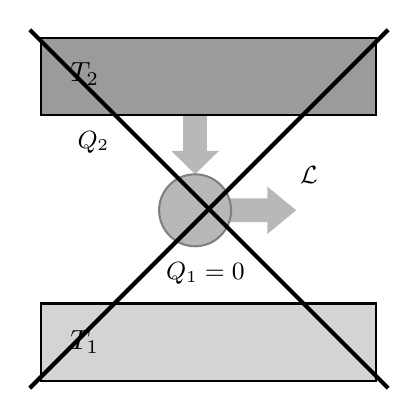
\begin{tikzpicture}[x=0.75pt,y=0.75pt,yscale=-1,xscale=1]
	%uncomment if require: \path (0,300); %set diagram left start at 0, and has height of 300

	%Right Arrow [id:dp8473176475298747] 
	\draw  [draw opacity=0][fill={rgb, 255:red, 184; green, 184; blue, 184 }  ,fill opacity=1 ] (180.06,84.5) -- (180.06,101.38) -- (185.8,101.38) -- (174.33,112.64) -- (162.87,101.38) -- (168.6,101.38) -- (168.6,84.5) -- cycle ;
	%Right Arrow [id:dp6689782123318382] 
	\draw  [draw opacity=0][fill={rgb, 255:red, 184; green, 184; blue, 184 }  ,fill opacity=1 ] (188.25,124.24) -- (209.1,124.24) -- (209.1,118.51) -- (223,129.97) -- (209.1,141.44) -- (209.1,135.7) -- (188.25,135.7) -- cycle ;
	%Shape: Rectangle [id:dp8418322748956599] 
	\draw  [fill={rgb, 255:red, 155; green, 155; blue, 155 }  ,fill opacity=1 ] (100,47) -- (261.5,47) -- (261.5,84.27) -- (100,84.27) -- cycle ;
	%Shape: Rectangle [id:dp6532511543396138] 
	\draw  [fill={rgb, 255:red, 212; green, 212; blue, 212 }  ,fill opacity=1 ] (100,174.9) -- (261.5,174.9) -- (261.5,212.17) -- (100,212.17) -- cycle ;
	%Shape: Ellipse [id:dp021022255460882988] 
	\draw  [color={rgb, 255:red, 128; green, 128; blue, 128 }  ,draw opacity=1 ][fill={rgb, 255:red, 184; green, 184; blue, 184 }  ,fill opacity=1 ] (157,129.97) .. controls (157,120.4) and (164.76,112.64) .. (174.33,112.64) .. controls (183.91,112.64) and (191.67,120.4) .. (191.67,129.97) .. controls (191.67,139.55) and (183.91,147.31) .. (174.33,147.31) .. controls (164.76,147.31) and (157,139.55) .. (157,129.97) -- cycle ;
	\draw  [line width=1.5]  (94.67,43) -- (267.33,215.67)(267.33,43) -- (94.67,215.67) ;

	% Text Node
	\draw (121.12,64.39) node    {$T_{2}$};
	% Text Node
	\draw (121.12,193.53) node    {$T_{1}$};
	% Text Node
	\draw (229.13,112.93) node  [font=\small]  {$\mathcal{L}$};
	% Text Node
	\draw (125.33,97.07) node  [font=\small]  {$Q_{2}$};
	% Text Node
	\draw (179.33,160.4) node  [font=\small]  {$Q_{1} =0$};

	\end{tikzpicture}
\end{figure}
\FloatBarrier
Non si può assorbire calore da un serbatoio per farlo diventare totalmente lavoro. Diretta conseguenza di questo risultato è che il rendimento della macchina termica deve essere strettamente minore di $1$. Si dovrà sempre avere che una frazione del calore assorbito non diventa lavoro ma rimane calore.

\textbf{Enunciato di Clausius}

\noindent\fbox{%
	\parbox{\textwidth}{%
		\emph{Non è possibile realizzare un processo il cui unico risultato sia il passaggio spontaneo di calore da un corpo più freddo a uno più caldo.}
	}%
}

Non si può avere un flusso di calore spontaneo che va da un corpo più freddo a uno più caldo.

Questi due enunciati hanno valenza molto pratica perché servono a dare una spiegazione ai limiti della macchina termica e all'efficienza della macchina frigorifera. Si può dimostrare che i due principi sono equivalenti. La dimostrazione procede per assurdo: negando la tesi enunciata da Kelvin e si ottiene la negazione dell'enunciato di Clausius. Si fa poi il viceversa. Se negando l'uno si nega anche l'altro in entrambi i sensi, vuol dire che i due concetti sono equivalenti.

\textbf{Dimostrazione}
\\

\textbf{Prima parte} Si immagini di poter realizzare un processo che va contro l'enunciato di Kelvin e quindi una macchina termica $NK$ che per assurdo trasforma tutto il calore $Q$ in lavoro $\mathcal{L}$.

\[
	Q = \mathcal{L}
\]

Si associ a questa macchina una frigorifera $F$ vera che lavora assorbendo il calore $Q_1$ da un serbatoio freddo $T_1$ e che, sfruttando un certo lavoro fornito dall'esterno, cede calore $Q_2$ al serbatoio $T_2$. Questa macchina frigorifera la si fa funzionare sfruttando il lavoro compiuto da $NK$.

\begin{figure}[htpb]
	\centering

	\tikzset{every picture/.style={line width=0.75pt}} %set default line width to 0.75pt        

	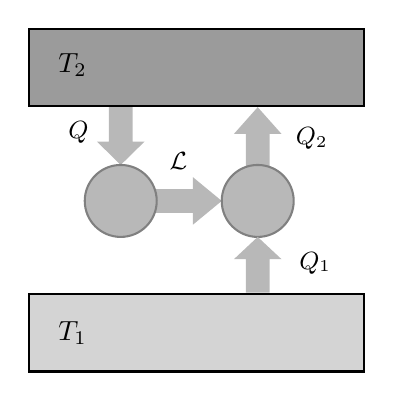
\begin{tikzpicture}[x=0.75pt,y=0.75pt,yscale=-1,xscale=1]
	%uncomment if require: \path (0,300); %set diagram left start at 0, and has height of 300

	%Right Arrow [id:dp692823662524541] 
	\draw  [draw opacity=0][fill={rgb, 255:red, 184; green, 184; blue, 184 }  ,fill opacity=1 ] (140.06,115.5) -- (140.06,132.38) -- (145.8,132.38) -- (134.33,143.64) -- (122.87,132.38) -- (128.6,132.38) -- (128.6,115.5) -- cycle ;
	%Right Arrow [id:dp9520394667646055] 
	\draw  [draw opacity=0][fill={rgb, 255:red, 184; green, 184; blue, 184 }  ,fill opacity=1 ] (194.6,148) -- (194.6,128.68) -- (188.87,128.68) -- (200.33,115.8) -- (211.8,128.68) -- (206.06,128.68) -- (206.06,148) -- cycle ;
	%Right Arrow [id:dp7108011204164864] 
	\draw  [draw opacity=0][fill={rgb, 255:red, 184; green, 184; blue, 184 }  ,fill opacity=1 ] (148.25,155.24) -- (169.1,155.24) -- (169.1,149.51) -- (183,160.97) -- (169.1,172.44) -- (169.1,166.7) -- (148.25,166.7) -- cycle ;
	%Shape: Rectangle [id:dp963014804190296] 
	\draw  [fill={rgb, 255:red, 155; green, 155; blue, 155 }  ,fill opacity=1 ] (90,78) -- (251.5,78) -- (251.5,115.27) -- (90,115.27) -- cycle ;
	%Shape: Rectangle [id:dp8078240816003164] 
	\draw  [fill={rgb, 255:red, 212; green, 212; blue, 212 }  ,fill opacity=1 ] (90,205.9) -- (251.5,205.9) -- (251.5,243.17) -- (90,243.17) -- cycle ;
	%Shape: Ellipse [id:dp6515968584185239] 
	\draw  [color={rgb, 255:red, 128; green, 128; blue, 128 }  ,draw opacity=1 ][fill={rgb, 255:red, 184; green, 184; blue, 184 }  ,fill opacity=1 ] (117,160.97) .. controls (117,151.4) and (124.76,143.64) .. (134.33,143.64) .. controls (143.91,143.64) and (151.67,151.4) .. (151.67,160.97) .. controls (151.67,170.55) and (143.91,178.31) .. (134.33,178.31) .. controls (124.76,178.31) and (117,170.55) .. (117,160.97) -- cycle ;
	%Shape: Ellipse [id:dp8113810604920477] 
	\draw  [color={rgb, 255:red, 128; green, 128; blue, 128 }  ,draw opacity=1 ][fill={rgb, 255:red, 184; green, 184; blue, 184 }  ,fill opacity=1 ] (183,160.97) .. controls (183,151.4) and (190.76,143.64) .. (200.33,143.64) .. controls (209.91,143.64) and (217.67,151.4) .. (217.67,160.97) .. controls (217.67,170.55) and (209.91,178.31) .. (200.33,178.31) .. controls (190.76,178.31) and (183,170.55) .. (183,160.97) -- cycle ;
	%Right Arrow [id:dp014211227584000286] 
	\draw  [draw opacity=0][fill={rgb, 255:red, 184; green, 184; blue, 184 }  ,fill opacity=1 ] (194.6,205.15) -- (194.6,189.04) -- (188.87,189.04) -- (200.33,178.31) -- (211.8,189.04) -- (206.06,189.04) -- (206.06,205.15) -- cycle ;

	% Text Node
	\draw (111.12,95.39) node    {$T_{2}$};
	% Text Node
	\draw (111.12,224.53) node    {$T_{1}$};
	% Text Node
	\draw (226.37,131.03) node  [font=\small]  {$Q_{2}$};
	% Text Node
	\draw (228,190.87) node  [font=\small]  {$Q_{1}$};
	% Text Node
	\draw (162.13,141.93) node  [font=\small]  {$\mathcal{L}$};
	% Text Node
	\draw (114,128.07) node  [font=\small]  {$Q$};

	\end{tikzpicture}
\end{figure}
\FloatBarrier
Il lavoro compiuto sulla macchina frigorifera, negativo, sarà uguale alla somma dei calori scambiati.

\[
	-\mathcal{L} = Q_1-|Q_2|
\]

Si consideri la macchina complessiva $NK+F$ e si mettano in evidenza i flussi energetici che entrano ed escono.

\begin{figure}[htpb]
	\centering

	\tikzset{every picture/.style={line width=0.75pt}} %set default line width to 0.75pt        

	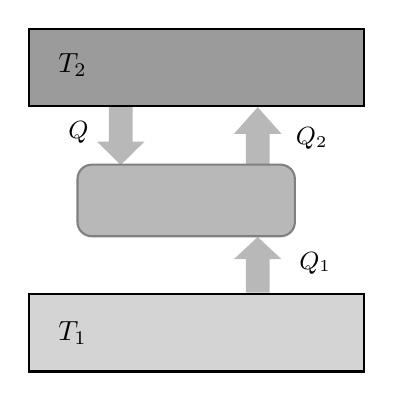
\begin{tikzpicture}[x=0.75pt,y=0.75pt,yscale=-1,xscale=1]
	%uncomment if require: \path (0,300); %set diagram left start at 0, and has height of 300

	%Right Arrow [id:dp5710645086709427] 
	\draw  [draw opacity=0][fill={rgb, 255:red, 184; green, 184; blue, 184 }  ,fill opacity=1 ] (140.06,115.5) -- (140.06,132.38) -- (145.8,132.38) -- (134.33,143.64) -- (122.87,132.38) -- (128.6,132.38) -- (128.6,115.5) -- cycle ;
	%Right Arrow [id:dp1360586020769976] 
	\draw  [draw opacity=0][fill={rgb, 255:red, 184; green, 184; blue, 184 }  ,fill opacity=1 ] (194.6,148) -- (194.6,128.68) -- (188.87,128.68) -- (200.33,115.8) -- (211.8,128.68) -- (206.06,128.68) -- (206.06,148) -- cycle ;
	%Shape: Rectangle [id:dp49710259570510074] 
	\draw  [fill={rgb, 255:red, 155; green, 155; blue, 155 }  ,fill opacity=1 ] (90,78) -- (251.5,78) -- (251.5,115.27) -- (90,115.27) -- cycle ;
	%Shape: Rectangle [id:dp9725838477858029] 
	\draw  [fill={rgb, 255:red, 212; green, 212; blue, 212 }  ,fill opacity=1 ] (90,205.9) -- (251.5,205.9) -- (251.5,243.17) -- (90,243.17) -- cycle ;
	%Right Arrow [id:dp3142970613204923] 
	\draw  [draw opacity=0][fill={rgb, 255:red, 184; green, 184; blue, 184 }  ,fill opacity=1 ] (194.6,205.15) -- (194.6,189.04) -- (188.87,189.04) -- (200.33,178.31) -- (211.8,189.04) -- (206.06,189.04) -- (206.06,205.15) -- cycle ;
	%Rounded Rect [id:dp3923655510821018] 
	\draw  [color={rgb, 255:red, 128; green, 128; blue, 128 }  ,draw opacity=1 ][fill={rgb, 255:red, 184; green, 184; blue, 184 }  ,fill opacity=1 ] (113.5,150.4) .. controls (113.5,146.59) and (116.59,143.5) .. (120.4,143.5) -- (211.35,143.5) .. controls (215.16,143.5) and (218.25,146.59) .. (218.25,150.4) -- (218.25,171.1) .. controls (218.25,174.91) and (215.16,178) .. (211.35,178) -- (120.4,178) .. controls (116.59,178) and (113.5,174.91) .. (113.5,171.1) -- cycle ;

	% Text Node
	\draw (111.12,95.39) node    {$T_{2}$};
	% Text Node
	\draw (111.12,224.53) node    {$T_{1}$};
	% Text Node
	\draw (226.37,131.03) node  [font=\small]  {$Q_{2}$};
	% Text Node
	\draw (228,190.87) node  [font=\small]  {$Q_{1}$};
	% Text Node
	\draw (114,128.07) node  [font=\small]  {$Q$};

	\end{tikzpicture}
\end{figure}
\FloatBarrier
Si avranno un calore $Q$ e un calore $Q_1$ che entrano nella macchina complessiva. Essa non compie un lavoro netto, sull'ambiente esterno, perché tutto il lavoro compiuto da una macchina viene immesso nell'altra macchina. Indicando con il pedice ‘totale' i flussi energetici caratterizzati dalla macchina totale, si ha:

\[
	\mathcal{L}_{\text{tot} } = 0
\]

Il calore totale scambiato con il serbatoio freddo è $Q_1$, positivo. $Q_{1,\text{tot}} = Q_1$. Il calore scambiato con il serbatoio caldo è $Q_{2,\text{tot}} = Q - |Q_2|$.

\[
	\left\{ \begin{array}{l}
	 	\text{macchina 1:}\quad Q = \mathcal{L}   \\
	 	\text{macchina 2:}\quad \mathcal{L} = - Q_1+|Q_2|
	\end{array} \right.
						\implies Q_1 = |Q_2| - Q > 0
\]

Quindi

\[
	Q_{2,\text{tot} } = Q - |Q_2| = - Q_{1,\text{tot}}
\]

Nella macchina totale il calore scambiato con il serbatoio caldo è uguale in modulo a quello scambiato con il serbatoio freddo. Il flusso spontaneo di calore avviene dal serbatoio caldo a quello freddo: negando Kelvin si è ottenuta di conseguenza una macchina che nega l'enunciato di Clausius.

\textbf{Seconda parte.} Si verifica ora che negando Clausius si ottiene la negazione di Kelvin. Si immagini di poter assorbire il calore dal serbatoio freddo al serbatoio caldo con una macchina $NC$. Si affianca ad essa una macchina termica $K$ che lavora a contatto con gli stessi due serbatoi ma che non va a negare Kelvin. Si scelga $K$ in modo tale che assorba una quantità $Q_2$ e ceda una quantità $Q_1=-Q$.

\begin{figure}[htpb]
	\centering

	\tikzset{every picture/.style={line width=0.75pt}} %set default line width to 0.75pt        

	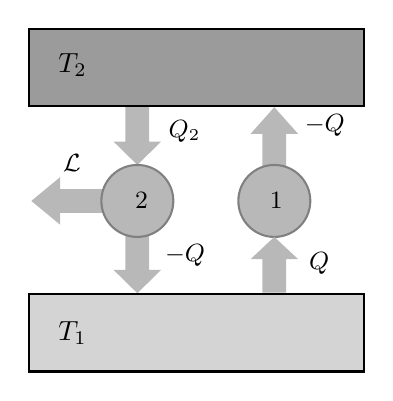
\begin{tikzpicture}[x=0.75pt,y=0.75pt,yscale=-1,xscale=1]
	%uncomment if require: \path (0,300); %set diagram left start at 0, and has height of 300

	%Right Arrow [id:dp268809622033948] 
	\draw  [draw opacity=0][fill={rgb, 255:red, 184; green, 184; blue, 184 }  ,fill opacity=1 ] (148.06,177.31) -- (148.06,194.19) -- (153.8,194.19) -- (142.33,205.45) -- (130.87,194.19) -- (136.6,194.19) -- (136.6,177.31) -- cycle ;
	%Right Arrow [id:dp05476736131166793] 
	\draw  [draw opacity=0][fill={rgb, 255:red, 184; green, 184; blue, 184 }  ,fill opacity=1 ] (148.06,115.5) -- (148.06,132.38) -- (153.8,132.38) -- (142.33,143.64) -- (130.87,132.38) -- (136.6,132.38) -- (136.6,115.5) -- cycle ;
	%Right Arrow [id:dp8241569512435416] 
	\draw  [draw opacity=0][fill={rgb, 255:red, 184; green, 184; blue, 184 }  ,fill opacity=1 ] (202.6,148) -- (202.6,128.68) -- (196.87,128.68) -- (208.33,115.8) -- (219.8,128.68) -- (214.06,128.68) -- (214.06,148) -- cycle ;
	%Right Arrow [id:dp7600028656618931] 
	\draw  [draw opacity=0][fill={rgb, 255:red, 184; green, 184; blue, 184 }  ,fill opacity=1 ] (126,166.7) -- (105.15,166.7) -- (105.15,172.44) -- (91.25,160.97) -- (105.15,149.51) -- (105.15,155.24) -- (126,155.24) -- cycle ;
	%Shape: Rectangle [id:dp5660737159746674] 
	\draw  [fill={rgb, 255:red, 155; green, 155; blue, 155 }  ,fill opacity=1 ] (90,78) -- (251.5,78) -- (251.5,115.27) -- (90,115.27) -- cycle ;
	%Shape: Rectangle [id:dp24441080398563697] 
	\draw  [fill={rgb, 255:red, 212; green, 212; blue, 212 }  ,fill opacity=1 ] (90,205.9) -- (251.5,205.9) -- (251.5,243.17) -- (90,243.17) -- cycle ;
	%Shape: Ellipse [id:dp7470281204567384] 
	\draw  [color={rgb, 255:red, 128; green, 128; blue, 128 }  ,draw opacity=1 ][fill={rgb, 255:red, 184; green, 184; blue, 184 }  ,fill opacity=1 ] (125,160.97) .. controls (125,151.4) and (132.76,143.64) .. (142.33,143.64) .. controls (151.91,143.64) and (159.67,151.4) .. (159.67,160.97) .. controls (159.67,170.55) and (151.91,178.31) .. (142.33,178.31) .. controls (132.76,178.31) and (125,170.55) .. (125,160.97) -- cycle ;
	%Shape: Ellipse [id:dp024660173797947715] 
	\draw  [color={rgb, 255:red, 128; green, 128; blue, 128 }  ,draw opacity=1 ][fill={rgb, 255:red, 184; green, 184; blue, 184 }  ,fill opacity=1 ] (191,160.97) .. controls (191,151.4) and (198.76,143.64) .. (208.33,143.64) .. controls (217.91,143.64) and (225.67,151.4) .. (225.67,160.97) .. controls (225.67,170.55) and (217.91,178.31) .. (208.33,178.31) .. controls (198.76,178.31) and (191,170.55) .. (191,160.97) -- cycle ;
	%Right Arrow [id:dp8055782873837063] 
	\draw  [draw opacity=0][fill={rgb, 255:red, 184; green, 184; blue, 184 }  ,fill opacity=1 ] (202.6,205.15) -- (202.6,189.04) -- (196.87,189.04) -- (208.33,178.31) -- (219.8,189.04) -- (214.06,189.04) -- (214.06,205.15) -- cycle ;

	% Text Node
	\draw (111.12,95.39) node    {$T_{2}$};
	% Text Node
	\draw (111.12,224.53) node    {$T_{1}$};
	% Text Node
	\draw (165.03,127.7) node  [font=\small]  {$Q_{2}$};
	% Text Node
	\draw (230,190.87) node  [font=\small]  {$Q$};
	% Text Node
	\draw (110.8,142.6) node  [font=\small]  {$\mathcal{L}$};
	% Text Node
	\draw (165.33,187.4) node  [font=\small]  {$-Q$};
	% Text Node
	\draw (232.67,124.73) node  [font=\small]  {$-Q$};
	% Text Node
	\draw (144.33,160.97) node  [font=\small]  {$2$};
	% Text Node
	\draw (209.33,160.97) node  [font=\small]  {$1$};

	\end{tikzpicture}
\end{figure}
\FloatBarrier
Si scrive il primo principio della termodinamica per la macchina $K$, la quale compie il lavoro $	\mathcal{L}$ positivo, frutto del fatto che va ad assorbire la quantità di calore $Q_2$ e a cedere la quantità di calore $Q$.

\[
	Q_2 - Q = \mathcal{L}
\]

Si consideri ora nuovamente la macchina complessiva, $NC+K$ e se ne mettano in evidenza i flussi energetici complessivi. Essa al netto compie un lavoro positivo.

\[
	Q_2 - Q = \mathcal{L}_\text{tot}
\]

Con il serbatoio freddo al netto non scambia calore perché $Q-Q=0$. Con il serbatoio caldo essa assorbe $Q_2$ e cede $-Q$.

\begin{align*}
	Q_{1,\text{tot}} &= 0 \\
	Q_{2,\text{tot} } &= Q_2 - Q
\end{align*}

Ma quest'ultima quantità è pari proprio al lavoro $\mathcal{L}_\text{tot}$ compiuto dalla macchina. Si è ottenuto che la macchina trasforma tutto il calore in lavoro.

\begin{figure}[htpb]
	\centering

	\tikzset{every picture/.style={line width=0.75pt}} %set default line width to 0.75pt        

	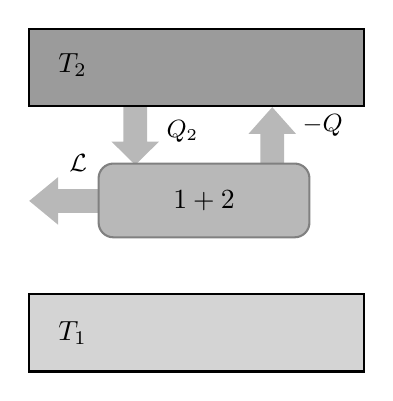
\begin{tikzpicture}[x=0.75pt,y=0.75pt,yscale=-1,xscale=1]
	%uncomment if require: \path (0,300); %set diagram left start at 0, and has height of 300

	%Right Arrow [id:dp5160310102780998] 
	\draw  [draw opacity=0][fill={rgb, 255:red, 184; green, 184; blue, 184 }  ,fill opacity=1 ] (147.06,115.5) -- (147.06,132.38) -- (152.8,132.38) -- (141.33,143.64) -- (129.87,132.38) -- (135.6,132.38) -- (135.6,115.5) -- cycle ;
	%Right Arrow [id:dp30761105478774775] 
	\draw  [draw opacity=0][fill={rgb, 255:red, 184; green, 184; blue, 184 }  ,fill opacity=1 ] (201.6,148) -- (201.6,128.68) -- (195.87,128.68) -- (207.33,115.8) -- (218.8,128.68) -- (213.06,128.68) -- (213.06,148) -- cycle ;
	%Right Arrow [id:dp37627454612607414] 
	\draw  [draw opacity=0][fill={rgb, 255:red, 184; green, 184; blue, 184 }  ,fill opacity=1 ] (125,166.7) -- (104.15,166.7) -- (104.15,172.44) -- (90.25,160.97) -- (104.15,149.51) -- (104.15,155.24) -- (125,155.24) -- cycle ;
	%Shape: Rectangle [id:dp007829210220858362] 
	\draw  [fill={rgb, 255:red, 155; green, 155; blue, 155 }  ,fill opacity=1 ] (90,78) -- (251.5,78) -- (251.5,115.27) -- (90,115.27) -- cycle ;
	%Shape: Rectangle [id:dp6803658960832004] 
	\draw  [fill={rgb, 255:red, 212; green, 212; blue, 212 }  ,fill opacity=1 ] (90,205.9) -- (251.5,205.9) -- (251.5,243.17) -- (90,243.17) -- cycle ;
	%Rounded Rect [id:dp9221191705387033] 
	\draw  [color={rgb, 255:red, 128; green, 128; blue, 128 }  ,draw opacity=1 ][fill={rgb, 255:red, 184; green, 184; blue, 184 }  ,fill opacity=1 ] (123.67,150.08) .. controls (123.67,146.15) and (126.85,142.97) .. (130.77,142.97) -- (218.14,142.97) .. controls (222.07,142.97) and (225.25,146.15) .. (225.25,150.08) -- (225.25,171.39) .. controls (225.25,175.32) and (222.07,178.5) .. (218.14,178.5) -- (130.77,178.5) .. controls (126.85,178.5) and (123.67,175.32) .. (123.67,171.39) -- cycle ;

	% Text Node
	\draw (111.12,95.39) node    {$T_{2}$};
	% Text Node
	\draw (111.12,224.53) node    {$T_{1}$};
	% Text Node
	\draw (164.03,127.7) node  [font=\small]  {$Q_{2}$};
	% Text Node
	\draw (113.8,142.6) node  [font=\small]  {$\mathcal{L}$};
	% Text Node
	\draw (231.67,124.73) node  [font=\small]  {$-Q$};
	% Text Node
	\draw (174.46,160.74) node    {$1+2$};

	\end{tikzpicture}
\end{figure}
\FloatBarrier
Negando Clausius si è arrivati alla negazione di Kelvin-Planck. Questi due enunciati che sembrano parlare di cose differenti, sono in realtà equivalenti, dicono qualcosa di molto simile.

\paragraph{Esempio} Si supponga di avere un carrellino che striscia su un piano d'appoggio grazie ad un energia cinetica. Si ha inizialmente un movimento ordinato di tutte le parti del corpo, che si muovono tutte solidali in una direzione. Il piano avrà un certo attrito, quindi dopo un certo tempo il corpo si ferma. L'energia meccanica si è dissipata nel momento in cui esso strisciando ha messo in agitazione le molecole che si trovano sulla superficie di contatto, e che hanno iniziato a vibrare in maniera più rapida. Il primo principio della termodinamica non vieta di pensare che si potrebbe prendere il calore e realizzare in qualche maniera una macchina che permetta di utilizzare il calore ceduto al tavolo per ritrasformarlo in movimento ordinato del carrellino, che ricomincia a muoversi magari indietro, realizzando un moto perpetuo. In realtà si sa che questo processo non è realizzabile. È il secondo principio della termodinamica a porre quindi dei limiti ai passaggi di energia, che possono avvenire solo in certe direzioni: il calore non può mai ritrasformarsi tutto in lavoro. Questo semplice esempio propone allora una visione più generale del secondo principio della termodinamica, secondo la quale vi è sempre una tendenza spontanea dell'energia a passare da una forma più ordinata a una forma più disordinata. Spontaneamente il moto ordinato di particelle si trasforma in moto disordinato.

\paragraph{Osservazione} Perché il termine \emph{unico} che figura nell'enunciato di Clausius è importante? Quando si fa espandere un gas, ad esempio, in maniera isoterma, esso parte da uno stato iniziale, si espande, aumenta il volume e quindi fornisce lavoro all'ambiente circostante, sollevando il pistone. Questo lavoro lo fa assorbendo calore dal serbatoio con cui è a contatto.
Questo è un processo in cui in realtà sfruttando un calore fornito da un serbatoio lo si trasforma tutto in lavoro. Esso tuttavia non viola, come sembrerebbe, il secondo principio della termodinamica. Alla fine del processo infatti non si è più nello stato iniziale, esso è cambiato e se si volesse tornare indietro lungo la stessa trasformazione si avrebbe il passaggio inverso e tutto il lavoro prodotto ritornerebbe in calore. Quindi c'è stato un altro risultato oltre alla trasformazione di calore in lavoro: il passaggio ad un altro stato termodinamico.

\paragraph{Reversibilità e irreversibilità} Finora si è posta l'attenzione, ai fini della reversibilità o irreversibilità di un processo, alle caratteristiche di equilibrio degli stati termodinamici attraversati dal sistema. Si possono estendere tali considerazioni all'ambiente e dire che in generale una trasformazione reversibile non comporta alterazioni permanenti, nel senso che è sempre possibile riportare nei rispettivi stati iniziali il sistema e l'ambiente che con esso interagisce. Al contrario, quando avviene una trasformazione irreversibile, non è più possibile ritornare allo stato di partenza senza modificare il resto dell'universo. Il sistema può anche essere riportato allo stato iniziale attraverso altre trasformazioni, ma l'ambiente subisce una modifica irreversibile. Nella pratica tutte le trasformazioni che avvengono in natura contengono fattori di irreversibilità. La rappresentazione di un fenomeno reale con una trasformazione reversibile costituisce quindi una idealizzazione del processo.

\section{Il teorema di Carnot}

Il secondo principio della termodinamica, da un punto di vista pratico, assume il significato di affermare che il rendimento di una macchina termica è strettamente minore di uno. Si può affiancare ad esso un teorema che prende il nome di \textbf{teorema di Carnot} che quantifica ancora meglio qual è il limite massimo al rendimento di una certa macchina termica (si tratta di una precisazione quantitativa dell'enunciato di Kelvin-Planck). In particolare si concentra solo su una specifica tipologia di macchine termiche, quelle che scambiano calore con due serbatoi, sia reversibili che irreversibili. Esso afferma che:

\noindent\fbox{%
	\parbox{\textwidth}{%
		\emph{Tutte le macchine reversibili che lavorano tra le stesse sorgenti alle temperature $T_1$ e $T_2$ hanno rendimento eguale; qualsiasi altra macchina che lavori tra le stesse sorgenti non può avere rendimento maggiore. Il risultato è indipendente dal particolare sistema che compie il ciclo}.
	}%
}

Dal momento che la macchina reversibile di Carnot ha come rendimento $1-T_1/T_2$ e che tutte le macchine reversibili operanti fra le stesse sorgenti e quindi fra le stesse temperature hanno rendimento uguale, si avrà che il rendimento di qualsiasi macchina reversibile è dato da:

\[
	\eta_{\text{rev} } = \eta_{\text{Carnot} } = 1 - \frac{T_1 }{T_2 }
\]

Tutte le macchine irreversibili hanno rendimento strettamente inferiore a quello della macchina reversibile operante fra i due serbatoi. Il teorema sta dicendo che si può arrivare a ottenere come rendimento massimo $1-T_1/T_2$.
Insomma, a parità di lavoro fornito, la macchina reversibile è quella che assorbe meno calore. Il teorema si scrive in maniera compatta come:

\[
	\boxed{\eta \le 1-\frac{T_1}{T_2}}
\]

\textbf{Dimostrazione}

La dimostrazione procede per assurdo. Visto che il teorema di Carnot confronta il rendimento di diverse macchine termiche, bisogna immaginare di averne almeno due da confrontare. Si ha la macchina termica $X$ qualunque (non si sa se sia reversibile o irreversibile). La si confronta con una seconda macchina termica $R$ che si ipotizza invece reversibile. Per semplicità di dimostrazione si ipotizza che il lavoro compiuto dalle due macchine sia lo stesso.

\begin{figure}[htpb]
	\centering

	\tikzset{every picture/.style={line width=0.75pt}} %set default line width to 0.75pt        

	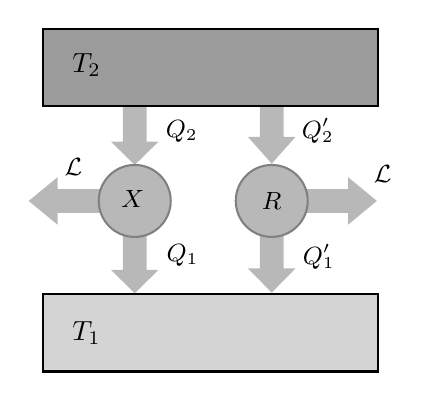
\begin{tikzpicture}[x=0.75pt,y=0.75pt,yscale=-1,xscale=1]
	%uncomment if require: \path (0,300); %set diagram left start at 0, and has height of 300

	%Right Arrow [id:dp912872186178135] 
	\draw  [draw opacity=0][fill={rgb, 255:red, 184; green, 184; blue, 184 }  ,fill opacity=1 ] (216.25,155.24) -- (237.1,155.24) -- (237.1,149.51) -- (251,160.97) -- (237.1,172.44) -- (237.1,166.7) -- (216.25,166.7) -- cycle ;
	%Right Arrow [id:dp6510841063831212] 
	\draw  [draw opacity=0][fill={rgb, 255:red, 184; green, 184; blue, 184 }  ,fill opacity=1 ] (140.06,177.31) -- (140.06,194.19) -- (145.8,194.19) -- (134.33,205.45) -- (122.87,194.19) -- (128.6,194.19) -- (128.6,177.31) -- cycle ;
	%Right Arrow [id:dp942922084825111] 
	\draw  [draw opacity=0][fill={rgb, 255:red, 184; green, 184; blue, 184 }  ,fill opacity=1 ] (140.06,115.5) -- (140.06,132.38) -- (145.8,132.38) -- (134.33,143.64) -- (122.87,132.38) -- (128.6,132.38) -- (128.6,115.5) -- cycle ;
	%Right Arrow [id:dp1581025718322091] 
	\draw  [draw opacity=0][fill={rgb, 255:red, 184; green, 184; blue, 184 }  ,fill opacity=1 ] (206.06,110.8) -- (206.06,130.12) -- (211.8,130.12) -- (200.33,143) -- (188.87,130.12) -- (194.6,130.12) -- (194.6,110.8) -- cycle ;
	%Right Arrow [id:dp9259895328868126] 
	\draw  [draw opacity=0][fill={rgb, 255:red, 184; green, 184; blue, 184 }  ,fill opacity=1 ] (118,166.7) -- (97.15,166.7) -- (97.15,172.44) -- (83.25,160.97) -- (97.15,149.51) -- (97.15,155.24) -- (118,155.24) -- cycle ;
	%Shape: Rectangle [id:dp6859292289839427] 
	\draw  [fill={rgb, 255:red, 155; green, 155; blue, 155 }  ,fill opacity=1 ] (90,78) -- (251.5,78) -- (251.5,115.27) -- (90,115.27) -- cycle ;
	%Shape: Rectangle [id:dp11183600044342779] 
	\draw  [fill={rgb, 255:red, 212; green, 212; blue, 212 }  ,fill opacity=1 ] (90,205.9) -- (251.5,205.9) -- (251.5,243.17) -- (90,243.17) -- cycle ;
	%Shape: Ellipse [id:dp25979482462928205] 
	\draw  [color={rgb, 255:red, 128; green, 128; blue, 128 }  ,draw opacity=1 ][fill={rgb, 255:red, 184; green, 184; blue, 184 }  ,fill opacity=1 ] (117,160.97) .. controls (117,151.4) and (124.76,143.64) .. (134.33,143.64) .. controls (143.91,143.64) and (151.67,151.4) .. (151.67,160.97) .. controls (151.67,170.55) and (143.91,178.31) .. (134.33,178.31) .. controls (124.76,178.31) and (117,170.55) .. (117,160.97) -- cycle ;
	%Right Arrow [id:dp6597263770006356] 
	\draw  [draw opacity=0][fill={rgb, 255:red, 184; green, 184; blue, 184 }  ,fill opacity=1 ] (206.06,176) -- (206.06,193.49) -- (211.8,193.49) -- (200.33,205.15) -- (188.87,193.49) -- (194.6,193.49) -- (194.6,176) -- cycle ;
	%Shape: Ellipse [id:dp1983125026578465] 
	\draw  [color={rgb, 255:red, 128; green, 128; blue, 128 }  ,draw opacity=1 ][fill={rgb, 255:red, 184; green, 184; blue, 184 }  ,fill opacity=1 ] (183,160.97) .. controls (183,151.4) and (190.76,143.64) .. (200.33,143.64) .. controls (209.91,143.64) and (217.67,151.4) .. (217.67,160.97) .. controls (217.67,170.55) and (209.91,178.31) .. (200.33,178.31) .. controls (190.76,178.31) and (183,170.55) .. (183,160.97) -- cycle ;

	% Text Node
	\draw (111.12,95.39) node    {$T_{2}$};
	% Text Node
	\draw (111.12,224.53) node    {$T_{1}$};
	% Text Node
	\draw (157.03,127.7) node  [font=\small]  {$Q_{2}$};
	% Text Node
	\draw (223,187.87) node  [font=\small]  {$Q'_{1}$};
	% Text Node
	\draw (104.8,144.6) node  [font=\small]  {$\mathcal{L}$};
	% Text Node
	\draw (157.33,187.4) node  [font=\small]  {$Q_{1}$};
	% Text Node
	\draw (222.53,127.2) node  [font=\small]  {$Q'_{2}$};
	% Text Node
	\draw (253.8,148.1) node  [font=\small]  {$\mathcal{L}$};
	% Text Node
	\draw (133.33,159.97) node  [font=\small]  {$X$};
	% Text Node
	\draw (200.33,160.97) node  [font=\small]  {$R$};

	\end{tikzpicture}
\end{figure}
\FloatBarrier
Si scrive per $X$ e $R$ il primo principio della termodinamica:

\[
	\left. \begin{array}{l}
	 	X:\quad \mathcal{L} = Q_2 - |Q_1|  \\
		R:\quad \mathcal{L} = Q_2' - |Q_1'|
	\end{array} \right\}
	\quad Q_2 - |Q_1| = Q_2' - |Q_1'|
\]

Si nega per assurdo che $\eta_x \le \eta_{\text{Carnot}}$. Quindi si ipotizza che $\eta_x > \eta_{\text{Carnot}}$. Ciò significa affermare, dato che $R$ è reversibile, che: $\eta_X > \eta_R$.

\[
	\frac{\mathcal{L} }{Q_2 } > \frac{\mathcal{L} }{Q_2'} \implies Q_2' > Q_2
\]

Se si afferma che $X$ ha rendimento maggiore di $R$ anche se fanno lo stesso lavoro, la prima assorbirà meno calore. Ciò comporta che:

\[
	Q_2-Q_2' < 0 \quad \text{ma} \quad Q_2-Q_2' = |Q_1| - |Q_1'|
\]

E allora:

\[
	|Q_1| - |Q_1'| < 0
\]

Dire che $X$ ha rendimento maggiore di $R$ significa che a pari lavoro fatto bisogna cedere al serbatoio freddo meno calore di quello che cede $R$. Poichè $R$ è reversibile, nessuno vieta di invertirne i flussi energetici, di farla funzionare come un frigo e l'unica cosa che cambia sono i segni di tali flussi. Si vuole realizzare una macchina termica complessiva che sfrutta il lavoro fatto da $X$, lo immette nella macchina $-R$ ribaltato di segno. Si analizza quello che succede alla macchina complessiva formata da $X - R$. Essa non compie un lavoro complessivo perché tutto quello compiuto da $X$ viene assorbito da $-R$. Il calore scambiato con il serbatoio freddo è, dal punto di vista di $X-R$, maggiore di zero. La macchina $X-R$ scambia con il serbatoio freddo un calore $Q_1$ totale che è positivo. La quantità $Q_2$ scambiata con il serbatoio caldo è negativa, quindi è ceduta.

\[
	\mathcal{L}_{\text{tot} } = 0 \qquad Q_{1,\text{tot} } = |Q_1'| - Q > 0 \qquad Q_{2,\text{tot} } = Q_2 - Q_2' < 0
\]

Questo processo non è realizzabile perché nega l'enunciato di Clausius.

\begin{figure}[htpb]
	\centering

	\tikzset{every picture/.style={line width=0.75pt}} %set default line width to 0.75pt        

	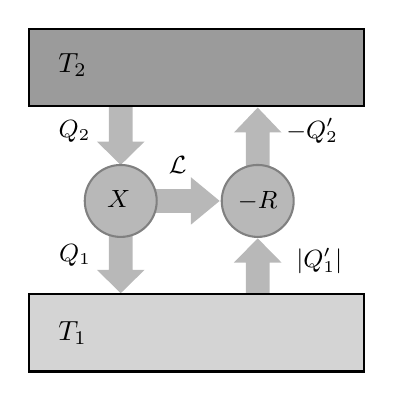
\begin{tikzpicture}[x=0.75pt,y=0.75pt,yscale=-1,xscale=1]
	%uncomment if require: \path (0,300); %set diagram left start at 0, and has height of 300

	%Right Arrow [id:dp6055110426069534] 
	\draw  [draw opacity=0][fill={rgb, 255:red, 184; green, 184; blue, 184 }  ,fill opacity=1 ] (194.6,208.15) -- (194.6,190.66) -- (188.87,190.66) -- (200.33,179) -- (211.8,190.66) -- (206.06,190.66) -- (206.06,208.15) -- cycle ;
	%Right Arrow [id:dp8251551468017688] 
	\draw  [draw opacity=0][fill={rgb, 255:red, 184; green, 184; blue, 184 }  ,fill opacity=1 ] (147.25,155.24) -- (168.1,155.24) -- (168.1,149.51) -- (182,160.97) -- (168.1,172.44) -- (168.1,166.7) -- (147.25,166.7) -- cycle ;
	%Right Arrow [id:dp05857966804666659] 
	\draw  [draw opacity=0][fill={rgb, 255:red, 184; green, 184; blue, 184 }  ,fill opacity=1 ] (140.06,177.31) -- (140.06,194.19) -- (145.8,194.19) -- (134.33,205.45) -- (122.87,194.19) -- (128.6,194.19) -- (128.6,177.31) -- cycle ;
	%Right Arrow [id:dp8971772094790116] 
	\draw  [draw opacity=0][fill={rgb, 255:red, 184; green, 184; blue, 184 }  ,fill opacity=1 ] (140.06,115.5) -- (140.06,132.38) -- (145.8,132.38) -- (134.33,143.64) -- (122.87,132.38) -- (128.6,132.38) -- (128.6,115.5) -- cycle ;
	%Right Arrow [id:dp3225172431020591] 
	\draw  [draw opacity=0][fill={rgb, 255:red, 184; green, 184; blue, 184 }  ,fill opacity=1 ] (194.6,146) -- (194.6,128) -- (188.87,128) -- (200.33,116) -- (211.8,128) -- (206.06,128) -- (206.06,146) -- cycle ;
	%Shape: Rectangle [id:dp152284570855713] 
	\draw  [fill={rgb, 255:red, 155; green, 155; blue, 155 }  ,fill opacity=1 ] (90,78) -- (251.5,78) -- (251.5,115.27) -- (90,115.27) -- cycle ;
	%Shape: Rectangle [id:dp0038282222062271387] 
	\draw  [fill={rgb, 255:red, 212; green, 212; blue, 212 }  ,fill opacity=1 ] (90,205.9) -- (251.5,205.9) -- (251.5,243.17) -- (90,243.17) -- cycle ;
	%Shape: Ellipse [id:dp07931735472955848] 
	\draw  [color={rgb, 255:red, 128; green, 128; blue, 128 }  ,draw opacity=1 ][fill={rgb, 255:red, 184; green, 184; blue, 184 }  ,fill opacity=1 ] (117,160.97) .. controls (117,151.4) and (124.76,143.64) .. (134.33,143.64) .. controls (143.91,143.64) and (151.67,151.4) .. (151.67,160.97) .. controls (151.67,170.55) and (143.91,178.31) .. (134.33,178.31) .. controls (124.76,178.31) and (117,170.55) .. (117,160.97) -- cycle ;
	%Shape: Ellipse [id:dp4662864673487097] 
	\draw  [color={rgb, 255:red, 128; green, 128; blue, 128 }  ,draw opacity=1 ][fill={rgb, 255:red, 184; green, 184; blue, 184 }  ,fill opacity=1 ] (183,160.97) .. controls (183,151.4) and (190.76,143.64) .. (200.33,143.64) .. controls (209.91,143.64) and (217.67,151.4) .. (217.67,160.97) .. controls (217.67,170.55) and (209.91,178.31) .. (200.33,178.31) .. controls (190.76,178.31) and (183,170.55) .. (183,160.97) -- cycle ;

	% Text Node
	\draw (111.12,95.39) node    {$T_{2}$};
	% Text Node
	\draw (111.12,224.53) node    {$T_{1}$};
	% Text Node
	\draw (112.03,127.7) node  [font=\small]  {$Q_{2}$};
	% Text Node
	\draw (230,189.87) node  [font=\small]  {$|Q'_{1} |$};
	% Text Node
	\draw (112.33,187.4) node  [font=\small]  {$Q_{1}$};
	% Text Node
	\draw (226.53,127.2) node  [font=\small]  {$-Q'_{2}$};
	% Text Node
	\draw (161.8,143.6) node  [font=\small]  {$\mathcal{L}$};
	% Text Node
	\draw (133.33,159.97) node  [font=\small]  {$X$};
	% Text Node
	\draw (200.33,160.97) node  [font=\small]  {$-R$};

	\end{tikzpicture}
\end{figure}
\FloatBarrier
Data una macchina $X$, avrà sempre rendimento minore o uguale di una qualunque macchina reversibile che lavora fra le stesse temperature.

\[
	\boxed{\eta_X \le \eta_{\text{Carnot} }}
\]

Si vuole anche dimostrare che se una macchina è reversibile, il suo rendimento è effettivamente uguale a quello della macchina di Carnot. Per farlo si ripete lo stesso procedimento tenendo conto del fatto che questa volta anche la macchina $X$ è reversibile. Si ipotizza per assurdo che esista una macchina $X$ reversibile che ha rendimento minore della macchina di Carnot.

\begin{figure}[htpb]
	\centering

	\tikzset{every picture/.style={line width=0.75pt}} %set default line width to 0.75pt        

	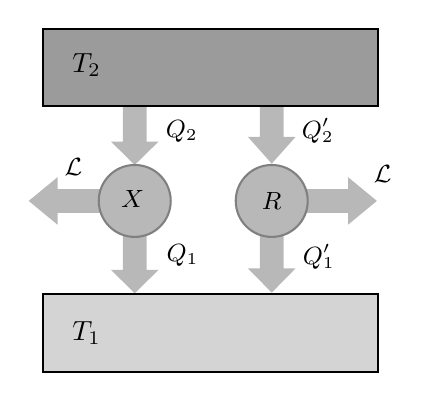
\begin{tikzpicture}[x=0.75pt,y=0.75pt,yscale=-1,xscale=1]
	%uncomment if require: \path (0,300); %set diagram left start at 0, and has height of 300

	%Right Arrow [id:dp06656680772679957] 
	\draw  [draw opacity=0][fill={rgb, 255:red, 184; green, 184; blue, 184 }  ,fill opacity=1 ] (236.25,175.24) -- (257.1,175.24) -- (257.1,169.51) -- (271,180.97) -- (257.1,192.44) -- (257.1,186.7) -- (236.25,186.7) -- cycle ;
	%Right Arrow [id:dp4295737856371209] 
	\draw  [draw opacity=0][fill={rgb, 255:red, 184; green, 184; blue, 184 }  ,fill opacity=1 ] (160.06,197.31) -- (160.06,214.19) -- (165.8,214.19) -- (154.33,225.45) -- (142.87,214.19) -- (148.6,214.19) -- (148.6,197.31) -- cycle ;
	%Right Arrow [id:dp004546700910957879] 
	\draw  [draw opacity=0][fill={rgb, 255:red, 184; green, 184; blue, 184 }  ,fill opacity=1 ] (160.06,135.5) -- (160.06,152.38) -- (165.8,152.38) -- (154.33,163.64) -- (142.87,152.38) -- (148.6,152.38) -- (148.6,135.5) -- cycle ;
	%Right Arrow [id:dp47307158531198845] 
	\draw  [draw opacity=0][fill={rgb, 255:red, 184; green, 184; blue, 184 }  ,fill opacity=1 ] (226.06,130.8) -- (226.06,150.12) -- (231.8,150.12) -- (220.33,163) -- (208.87,150.12) -- (214.6,150.12) -- (214.6,130.8) -- cycle ;
	%Right Arrow [id:dp7261559673782423] 
	\draw  [draw opacity=0][fill={rgb, 255:red, 184; green, 184; blue, 184 }  ,fill opacity=1 ] (138,186.7) -- (117.15,186.7) -- (117.15,192.44) -- (103.25,180.97) -- (117.15,169.51) -- (117.15,175.24) -- (138,175.24) -- cycle ;
	%Shape: Rectangle [id:dp25968617318137155] 
	\draw  [fill={rgb, 255:red, 155; green, 155; blue, 155 }  ,fill opacity=1 ] (110,98) -- (271.5,98) -- (271.5,135.27) -- (110,135.27) -- cycle ;
	%Shape: Rectangle [id:dp0412453343467456] 
	\draw  [fill={rgb, 255:red, 212; green, 212; blue, 212 }  ,fill opacity=1 ] (110,225.9) -- (271.5,225.9) -- (271.5,263.17) -- (110,263.17) -- cycle ;
	%Shape: Ellipse [id:dp0855071978115669] 
	\draw  [color={rgb, 255:red, 128; green, 128; blue, 128 }  ,draw opacity=1 ][fill={rgb, 255:red, 184; green, 184; blue, 184 }  ,fill opacity=1 ] (137,180.97) .. controls (137,171.4) and (144.76,163.64) .. (154.33,163.64) .. controls (163.91,163.64) and (171.67,171.4) .. (171.67,180.97) .. controls (171.67,190.55) and (163.91,198.31) .. (154.33,198.31) .. controls (144.76,198.31) and (137,190.55) .. (137,180.97) -- cycle ;
	%Right Arrow [id:dp5482255905886702] 
	\draw  [draw opacity=0][fill={rgb, 255:red, 184; green, 184; blue, 184 }  ,fill opacity=1 ] (226.06,196) -- (226.06,213.49) -- (231.8,213.49) -- (220.33,225.15) -- (208.87,213.49) -- (214.6,213.49) -- (214.6,196) -- cycle ;
	%Shape: Ellipse [id:dp7061906072557009] 
	\draw  [color={rgb, 255:red, 128; green, 128; blue, 128 }  ,draw opacity=1 ][fill={rgb, 255:red, 184; green, 184; blue, 184 }  ,fill opacity=1 ] (203,180.97) .. controls (203,171.4) and (210.76,163.64) .. (220.33,163.64) .. controls (229.91,163.64) and (237.67,171.4) .. (237.67,180.97) .. controls (237.67,190.55) and (229.91,198.31) .. (220.33,198.31) .. controls (210.76,198.31) and (203,190.55) .. (203,180.97) -- cycle ;

	% Text Node
	\draw (131.12,115.39) node    {$T_{2}$};
	% Text Node
	\draw (131.12,244.53) node    {$T_{1}$};
	% Text Node
	\draw (177.03,147.7) node  [font=\small]  {$Q_{2}$};
	% Text Node
	\draw (243,207.87) node  [font=\small]  {$Q'_{1}$};
	% Text Node
	\draw (124.8,164.6) node  [font=\small]  {$\mathcal{L}$};
	% Text Node
	\draw (177.33,207.4) node  [font=\small]  {$Q_{1}$};
	% Text Node
	\draw (242.53,147.2) node  [font=\small]  {$Q'_{2}$};
	% Text Node
	\draw (273.8,168.1) node  [font=\small]  {$\mathcal{L}$};
	% Text Node
	\draw (153.33,179.97) node  [font=\small]  {$X$};
	% Text Node
	\draw (220.33,180.97) node  [font=\small]  {$R$};

	\end{tikzpicture}
\end{figure}
\FloatBarrier
Si ha allora:

\begin{gather*}
	\frac{\mathcal{L} }{Q_2 } < \frac{\mathcal{L} }{Q_2'} \implies Q_2' < Q_2 \\
	\mathcal{L} = Q_2 - |Q_1| = Q_2' - |Q_1'| \implies \underbrace{Q_2 - Q_2'}_{>0} = \underbrace{|Q_1| - |Q_1'|}_{>0} \\
	|Q_1'| < |Q_1|
\end{gather*}

Visto che anche $X$ è reversibile, si può invertirne il funzionamento cambiando segno ai flussi energetici: $-X$. Si avrà la macchina $R+(-X)$.

\begin{figure}[htpb]
	\centering

	\tikzset{every picture/.style={line width=0.75pt}} %set default line width to 0.75pt        

	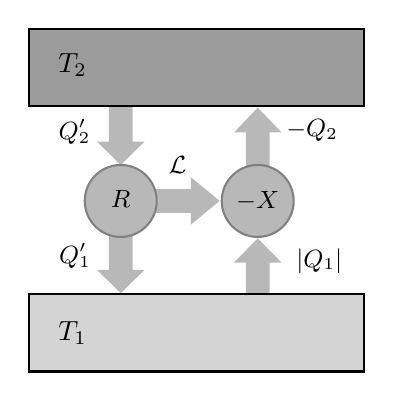
\begin{tikzpicture}[x=0.75pt,y=0.75pt,yscale=-1,xscale=1]
	%uncomment if require: \path (0,300); %set diagram left start at 0, and has height of 300

	%Right Arrow [id:dp5571594583875663] 
	\draw  [draw opacity=0][fill={rgb, 255:red, 184; green, 184; blue, 184 }  ,fill opacity=1 ] (194.6,208.15) -- (194.6,190.66) -- (188.87,190.66) -- (200.33,179) -- (211.8,190.66) -- (206.06,190.66) -- (206.06,208.15) -- cycle ;
	%Right Arrow [id:dp9701595242869454] 
	\draw  [draw opacity=0][fill={rgb, 255:red, 184; green, 184; blue, 184 }  ,fill opacity=1 ] (147.25,155.24) -- (168.1,155.24) -- (168.1,149.51) -- (182,160.97) -- (168.1,172.44) -- (168.1,166.7) -- (147.25,166.7) -- cycle ;
	%Right Arrow [id:dp5850403174906087] 
	\draw  [draw opacity=0][fill={rgb, 255:red, 184; green, 184; blue, 184 }  ,fill opacity=1 ] (140.06,177.31) -- (140.06,194.19) -- (145.8,194.19) -- (134.33,205.45) -- (122.87,194.19) -- (128.6,194.19) -- (128.6,177.31) -- cycle ;
	%Right Arrow [id:dp9065824176879271] 
	\draw  [draw opacity=0][fill={rgb, 255:red, 184; green, 184; blue, 184 }  ,fill opacity=1 ] (140.06,115.5) -- (140.06,132.38) -- (145.8,132.38) -- (134.33,143.64) -- (122.87,132.38) -- (128.6,132.38) -- (128.6,115.5) -- cycle ;
	%Right Arrow [id:dp09468071438501235] 
	\draw  [draw opacity=0][fill={rgb, 255:red, 184; green, 184; blue, 184 }  ,fill opacity=1 ] (194.6,146) -- (194.6,128) -- (188.87,128) -- (200.33,116) -- (211.8,128) -- (206.06,128) -- (206.06,146) -- cycle ;
	%Shape: Rectangle [id:dp19913563263937073] 
	\draw  [fill={rgb, 255:red, 155; green, 155; blue, 155 }  ,fill opacity=1 ] (90,78) -- (251.5,78) -- (251.5,115.27) -- (90,115.27) -- cycle ;
	%Shape: Rectangle [id:dp6157536168545994] 
	\draw  [fill={rgb, 255:red, 212; green, 212; blue, 212 }  ,fill opacity=1 ] (90,205.9) -- (251.5,205.9) -- (251.5,243.17) -- (90,243.17) -- cycle ;
	%Shape: Ellipse [id:dp9094909762729622] 
	\draw  [color={rgb, 255:red, 128; green, 128; blue, 128 }  ,draw opacity=1 ][fill={rgb, 255:red, 184; green, 184; blue, 184 }  ,fill opacity=1 ] (117,160.97) .. controls (117,151.4) and (124.76,143.64) .. (134.33,143.64) .. controls (143.91,143.64) and (151.67,151.4) .. (151.67,160.97) .. controls (151.67,170.55) and (143.91,178.31) .. (134.33,178.31) .. controls (124.76,178.31) and (117,170.55) .. (117,160.97) -- cycle ;
	%Shape: Ellipse [id:dp8941281519724829] 
	\draw  [color={rgb, 255:red, 128; green, 128; blue, 128 }  ,draw opacity=1 ][fill={rgb, 255:red, 184; green, 184; blue, 184 }  ,fill opacity=1 ] (183,160.97) .. controls (183,151.4) and (190.76,143.64) .. (200.33,143.64) .. controls (209.91,143.64) and (217.67,151.4) .. (217.67,160.97) .. controls (217.67,170.55) and (209.91,178.31) .. (200.33,178.31) .. controls (190.76,178.31) and (183,170.55) .. (183,160.97) -- cycle ;

	% Text Node
	\draw (111.12,95.39) node    {$T_{2}$};
	% Text Node
	\draw (111.12,224.53) node    {$T_{1}$};
	% Text Node
	\draw (112.03,127.7) node  [font=\small]  {$Q'_{2}$};
	% Text Node
	\draw (230,189.87) node  [font=\small]  {$|Q_{1} |$};
	% Text Node
	\draw (112.33,187.4) node  [font=\small]  {$Q'_{1}$};
	% Text Node
	\draw (226.53,127.2) node  [font=\small]  {$-Q_{2}$};
	% Text Node
	\draw (161.8,143.6) node  [font=\small]  {$\mathcal{L}$};
	% Text Node
	\draw (134.33,159.97) node  [font=\small]  {$R$};
	% Text Node
	\draw (200.33,160.97) node  [font=\small]  {$-X$};

	\end{tikzpicture}
\end{figure}
\FloatBarrier
Essa non compie lavoro perché quello realizzato dalla macchina $R$ è usato completamente dalla macchina $-X$. Le quantità

\[
	Q_{2,\text{tot} } = Q_2' - Q_2 < 0 \qquad Q_{1,\text{tot} } = |Q_1| - |Q_1'| > 0
\]

sono rispettivamente una negativa e l'altra positiva. Si sta realizzando una macchina in cui verso il serbatoio caldo arriva calore. La macchina viola l'enunciato di Clausius. Ciò significa che l'ipotesi di partenza $\eta_X< \eta_{\text{Carnot}}$ è assurda e quindi deve essere:

\[
	\eta_X \geq \eta_{\text{Carnot}}
\]

Ma per quanto dimostrato nella prima parte, si ha sempre:

\[
	\eta_X \leq \eta_{\text{Carnot}}
\]

Allora:

\[
	\left\{ \begin{array}{r}
	 	\eta_X \geq \eta_{\text{Carnot}} \\
		\eta_X \leq \eta_{\text{Carnot}}
	\end{array} \right.
	\implies \boxed{\eta_X = \eta_{\text{rev}} = \eta_{\text{Carnot}}}
\]

In sintesi:

\[
	\boxed{\eta_X \le \eta_{\text{Carnot} }\left\{ \begin{array}{l}
	 	\eta_X = \eta_{\text{Carnot} } = 1 - \frac{T_1 }{T_2 }\quad \text{se }X\text{ è reversibile} \\
		\eta_X < \eta_{\text{Carnot} } \quad \text{se }X\text{ è irreversibile}
	\end{array} \right.}
\]

Per dimostrare il teorema è stato usato uno dei due enunciati del secondo principio della termodinamica. Si potrebbe anche negare Clausius e arrivare alla negazione di Carnot. Questo indica che il teorema di Carnot è un altro modo per esprimere (un altro enunciato) il secondo principio della termodinamica ma ha lo stesso significato e porterà alla definizione della grandezza entropia.

\paragraph{Rendimento della macchina di Stirling} Si consideri la macchina di Stirling irreversibile. Si può sicuramente dire che il rendimento della macchina irreversibile è minore di $1-T_1/T_2$. Se lo stesso ciclo lo si esegue in maniera reversibile ci si può chiedere se questa macchina scambi effettivamente calore con solo due serbatoi. A occhio sembra di sì perché si hanno due isoterme a temperature diverse. Ma bisogna ragionare meglio su quello che accade nelle isocore.

\begin{figure}[htpb]
	\centering

	\tikzset{every picture/.style={line width=0.75pt}} %set default line width to 0.75pt        

	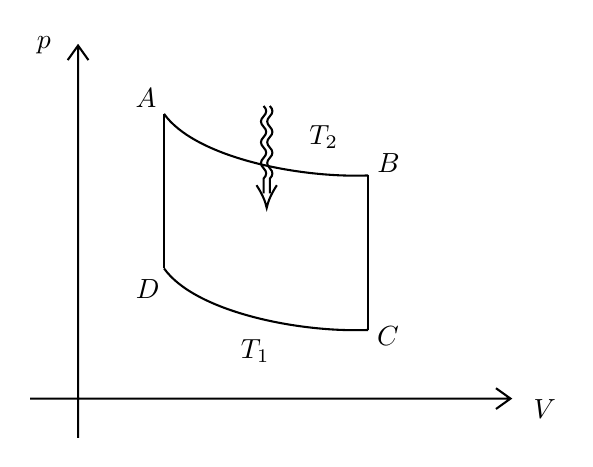
\begin{tikzpicture}[x=0.75pt,y=0.75pt,yscale=-1,xscale=1]
	%uncomment if require: \path (0,300); %set diagram left start at 0, and has height of 300

	%Shape: Axis 2D [id:dp5586747872942945] 
	\draw  (112,195.1) -- (343.5,195.1)(135.15,25) -- (135.15,214) (336.5,190.1) -- (343.5,195.1) -- (336.5,200.1) (130.15,32) -- (135.15,25) -- (140.15,32)  ;
	%Curve Lines [id:da9764359194008205] 
	\draw    (176.57,57.92) .. controls (191.27,78.63) and (240.8,88.92) .. (274.87,87.58) ;
	%Straight Lines [id:da42446695351819175] 
	\draw    (176.57,57.92) -- (176.57,132.37) ;
	%Curve Lines [id:da8065092271443957] 
	\draw    (176.57,132.37) .. controls (191.27,153.08) and (240.8,163.37) .. (274.87,162.03) ;
	%Straight Lines [id:da8598863477808285] 
	\draw    (274.87,87.58) -- (274.87,162.03) ;
	%Straight Lines [id:da8868732384234441] 
	\draw    (227.53,54.11) .. controls (229.2,55.78) and (229.2,57.44) .. (227.53,59.11) .. controls (225.86,60.78) and (225.86,62.44) .. (227.53,64.11) .. controls (229.2,65.78) and (229.2,67.44) .. (227.53,69.11) .. controls (225.86,70.78) and (225.86,72.44) .. (227.53,74.11) .. controls (229.2,75.78) and (229.2,77.44) .. (227.53,79.11) .. controls (225.86,80.78) and (225.86,82.44) .. (227.53,84.11) .. controls (229.2,85.78) and (229.2,87.44) .. (227.53,89.11) -- (227.53,93.22) -- (227.53,96.22)(224.53,54.11) .. controls (226.2,55.78) and (226.2,57.44) .. (224.53,59.11) .. controls (222.86,60.78) and (222.86,62.44) .. (224.53,64.11) .. controls (226.2,65.78) and (226.2,67.44) .. (224.53,69.11) .. controls (222.86,70.78) and (222.86,72.44) .. (224.53,74.11) .. controls (226.2,75.78) and (226.2,77.44) .. (224.53,79.11) .. controls (222.86,80.78) and (222.86,82.44) .. (224.53,84.11) .. controls (226.2,85.78) and (226.2,87.44) .. (224.53,89.11) -- (224.53,93.22) -- (224.53,96.22) ;
	\draw [shift={(226.03,103.22)}, rotate = 270] [color={rgb, 255:red, 0; green, 0; blue, 0 }  ][line width=0.75]    (10.93,-4.9) .. controls (6.95,-2.3) and (3.31,-0.67) .. (0,0) .. controls (3.31,0.67) and (6.95,2.3) .. (10.93,4.9)   ;

	% Text Node
	\draw (118.67,25) node    {$p$};
	% Text Node
	\draw (360,200) node    {$V$};
	% Text Node
	\draw (167.85,50.07) node    {$A$};
	% Text Node
	\draw (284.76,81.48) node    {$B$};
	% Text Node
	\draw (284.47,164.94) node    {$C$};
	% Text Node
	\draw (168.72,142.26) node    {$D$};
	% Text Node
	\draw (220.53,171.99) node    {$T_{1}$};
	% Text Node
	\draw (253.53,68.99) node    {$T_{2}$};

	\end{tikzpicture}
\end{figure}
\FloatBarrier
Si immagini di vedere come effettuare il raffreddamento isocoro da $B$ a $C$. Il gas è arrivato a espandersi a contatto con il serbatoio $T_2$. Non si può mettere il gas direttamente a contatto con il serbatoio $T_1$. Si immagini di effettuare il riscaldamento isocoro molto lentamente. Per fare ciò, invece che cambiare il serbatoio $T_2$ con il serbatoio $T_1$ in una sola volta, si mette il gas via via a contatto con un numero infinito di serbatoi a temperature via via sempre più basse, in modo che il passaggio da una temperatura all'altra sia continuo. Ecco allora che la macchina di Stirling reversibile non scambia calore con solo due serbatoi ma con un'infinità di essi. Di conseguenza, non si può confrontare il suo rendimento con quello della macchina di Carnot, che risulta essere l'unica macchina reversibile la quale scambia calore con due soli serbatoi. Il teorema di Carnot parla di macchine che operano fra \emph{due} sorgenti e, se il loro numero è maggiore, allora il rendimento è minore di $1-T_1/T_2$.

\section{Il teorema di Clausius}

Ci sono altri tipi di macchine di Carnot che operano scambiando calore con tre serbatoi. Si tratta di macchine di Carnot costituite da tre isoterme e tre adiabatiche e il loro rendimento \emph{non} è pari a $1-T_\text{min}/T_\text{max}$. Si può estendere quindi il teorema di Carnot al caso di macchine che scambiano calore con un numero $n$ di serbatoi e poi a quelle che scambiano calore con un numero infinito di serbatoi.

\begin{figure}[htpb]
	\centering

	\tikzset{every picture/.style={line width=0.75pt}} %set default line width to 0.75pt        

	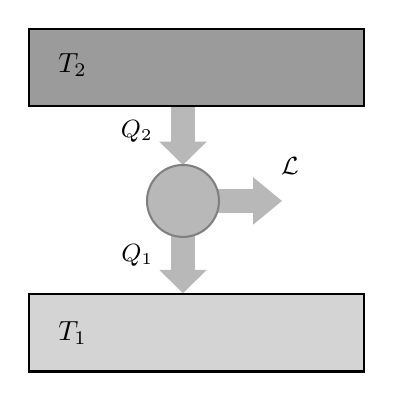
\begin{tikzpicture}[x=0.75pt,y=0.75pt,yscale=-1,xscale=1]
	%uncomment if require: \path (0,300); %set diagram left start at 0, and has height of 300

	%Right Arrow [id:dp06422156982176808] 
	\draw  [draw opacity=0][fill={rgb, 255:red, 184; green, 184; blue, 184 }  ,fill opacity=1 ] (177.25,155.24) -- (198.1,155.24) -- (198.1,149.51) -- (212,160.97) -- (198.1,172.44) -- (198.1,166.7) -- (177.25,166.7) -- cycle ;
	%Right Arrow [id:dp7080624294420244] 
	\draw  [draw opacity=0][fill={rgb, 255:red, 184; green, 184; blue, 184 }  ,fill opacity=1 ] (170.06,177.31) -- (170.06,194.19) -- (175.8,194.19) -- (164.33,205.45) -- (152.87,194.19) -- (158.6,194.19) -- (158.6,177.31) -- cycle ;
	%Right Arrow [id:dp5503612951569008] 
	\draw  [draw opacity=0][fill={rgb, 255:red, 184; green, 184; blue, 184 }  ,fill opacity=1 ] (170.06,115.5) -- (170.06,132.38) -- (175.8,132.38) -- (164.33,143.64) -- (152.87,132.38) -- (158.6,132.38) -- (158.6,115.5) -- cycle ;
	%Shape: Rectangle [id:dp41867474584744224] 
	\draw  [fill={rgb, 255:red, 155; green, 155; blue, 155 }  ,fill opacity=1 ] (90,78) -- (251.5,78) -- (251.5,115.27) -- (90,115.27) -- cycle ;
	%Shape: Rectangle [id:dp8775919710234561] 
	\draw  [fill={rgb, 255:red, 212; green, 212; blue, 212 }  ,fill opacity=1 ] (90,205.9) -- (251.5,205.9) -- (251.5,243.17) -- (90,243.17) -- cycle ;
	%Shape: Ellipse [id:dp41152320935778564] 
	\draw  [color={rgb, 255:red, 128; green, 128; blue, 128 }  ,draw opacity=1 ][fill={rgb, 255:red, 184; green, 184; blue, 184 }  ,fill opacity=1 ] (147,160.97) .. controls (147,151.4) and (154.76,143.64) .. (164.33,143.64) .. controls (173.91,143.64) and (181.67,151.4) .. (181.67,160.97) .. controls (181.67,170.55) and (173.91,178.31) .. (164.33,178.31) .. controls (154.76,178.31) and (147,170.55) .. (147,160.97) -- cycle ;

	% Text Node
	\draw (111.12,95.39) node    {$T_{2}$};
	% Text Node
	\draw (111.12,224.53) node    {$T_{1}$};
	% Text Node
	\draw (142.03,127.7) node  [font=\small]  {$Q_{2}$};
	% Text Node
	\draw (142.33,187.4) node  [font=\small]  {$Q_{1}$};
	% Text Node
	\draw (215.8,144.1) node  [font=\small]  {$\mathcal{L}$};

	\end{tikzpicture}
\end{figure}
\FloatBarrier
Il teorema di Carnot per $n=2$ serbatoi è dato da:

\[
	\eta_X = 1 - \frac{|Q_1|}{Q_2 } \le 1 - \frac{T_1 }{T_2 }
\]

Ricordando che $Q_1<0$:

\[
	\frac{Q_1 }{Q_2 } \le - \frac{T_1 }{T_2 }
\]

La relazione sta dicendo che, ricordandosi che le temperature sono sempre positive e che $Q_2$ è positivo, $Q_1$ è negativo, se la macchina $X$ è reversibile allora:

\begin{gather*}
	T_1>0 \implies \frac{Q_1 }{T_1 Q_2} \le - \frac{1}{T_2} \\
	Q_2>0 \implies \frac{Q_1 }{T_1 } \le - \frac{Q_2 }{T_2 } \\
	\frac{Q_1 }{T_1} + \frac{Q_2 }{T_2 } \le 0
\end{gather*}

Se la macchina $X$ è irreversibile il primo a termine è più negativo di quanto il secondo è positivo.

\[
	\frac{Q_1 }{T_1} + \frac{Q_2 }{T_2 } = 0 \quad (X\text{ rev} ) \qquad \frac{Q_1 }{T_1} + \frac{Q_2 }{T_2 } < 0 \quad (X\text{ irrev} )
\]

A questo punto tale risultato si estende al caso $n>2$ dicendo la sommatoria estesa a tutti gli $n$ serbatoi con cui la macchina ciclica sta scambiando calore, delle quantità $Q_i/T_i$ deve essere minore o al limite uguale a $0$. L'uguale vale se $X$ è reversibile, il minore se è irreversibile.

\begin{figure}[htpb]
	\centering

	\tikzset{every picture/.style={line width=0.75pt}} %set default line width to 0.75pt        

	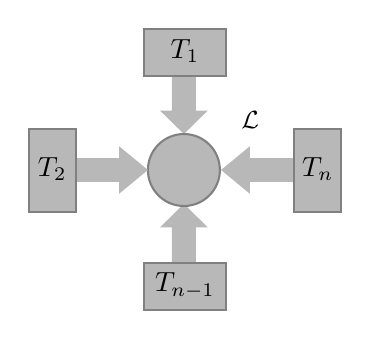
\begin{tikzpicture}[x=0.75pt,y=0.75pt,yscale=-1,xscale=1]
	%uncomment if require: \path (0,300); %set diagram left start at 0, and has height of 300

	%Right Arrow [id:dp2833606865986553] 
	\draw  [draw opacity=0][fill={rgb, 255:red, 184; green, 184; blue, 184 }  ,fill opacity=1 ] (217,166.7) -- (196.15,166.7) -- (196.15,172.44) -- (182.25,160.97) -- (196.15,149.51) -- (196.15,155.24) -- (217,155.24) -- cycle ;
	%Right Arrow [id:dp24042892933630888] 
	\draw  [draw opacity=0][fill={rgb, 255:red, 184; green, 184; blue, 184 }  ,fill opacity=1 ] (158.6,205.45) -- (158.6,188.56) -- (152.87,188.56) -- (164.33,177.31) -- (175.8,188.56) -- (170.06,188.56) -- (170.06,205.45) -- cycle ;
	%Right Arrow [id:dp784876077397787] 
	\draw  [draw opacity=0][fill={rgb, 255:red, 184; green, 184; blue, 184 }  ,fill opacity=1 ] (170.06,115.5) -- (170.06,132.38) -- (175.8,132.38) -- (164.33,143.64) -- (152.87,132.38) -- (158.6,132.38) -- (158.6,115.5) -- cycle ;
	%Shape: Rectangle [id:dp6297204887164671] 
	\draw  [color={rgb, 255:red, 128; green, 128; blue, 128 }  ,draw opacity=1 ][fill={rgb, 255:red, 184; green, 184; blue, 184 }  ,fill opacity=1 ] (145,205.9) -- (184.75,205.9) -- (184.75,228.5) -- (145,228.5) -- cycle ;
	%Shape: Ellipse [id:dp16335549952306083] 
	\draw  [color={rgb, 255:red, 128; green, 128; blue, 128 }  ,draw opacity=1 ][fill={rgb, 255:red, 184; green, 184; blue, 184 }  ,fill opacity=1 ] (147,160.97) .. controls (147,151.4) and (154.76,143.64) .. (164.33,143.64) .. controls (173.91,143.64) and (181.67,151.4) .. (181.67,160.97) .. controls (181.67,170.55) and (173.91,178.31) .. (164.33,178.31) .. controls (154.76,178.31) and (147,170.55) .. (147,160.97) -- cycle ;
	%Right Arrow [id:dp4503207186581166] 
	\draw  [draw opacity=0][fill={rgb, 255:red, 184; green, 184; blue, 184 }  ,fill opacity=1 ] (112.25,155.24) -- (133.1,155.24) -- (133.1,149.51) -- (147,160.97) -- (133.1,172.44) -- (133.1,166.7) -- (112.25,166.7) -- cycle ;
	%Shape: Rectangle [id:dp7742211356142767] 
	\draw  [color={rgb, 255:red, 128; green, 128; blue, 128 }  ,draw opacity=1 ][fill={rgb, 255:red, 184; green, 184; blue, 184 }  ,fill opacity=1 ] (145,92.9) -- (184.75,92.9) -- (184.75,115.5) -- (145,115.5) -- cycle ;
	%Shape: Rectangle [id:dp2203924120705476] 
	\draw  [color={rgb, 255:red, 128; green, 128; blue, 128 }  ,draw opacity=1 ][fill={rgb, 255:red, 184; green, 184; blue, 184 }  ,fill opacity=1 ] (240.18,141.32) -- (240.18,181.07) -- (217.57,181.07) -- (217.57,141.32) -- cycle ;
	%Shape: Rectangle [id:dp2882355114293944] 
	\draw  [color={rgb, 255:red, 128; green, 128; blue, 128 }  ,draw opacity=1 ][fill={rgb, 255:red, 184; green, 184; blue, 184 }  ,fill opacity=1 ] (112.18,141.32) -- (112.18,181.07) -- (89.57,181.07) -- (89.57,141.32) -- cycle ;

	% Text Node
	\draw (164.88,216.7) node    {$T_{n-1}$};
	% Text Node
	\draw (196.3,137.1) node  [font=\small]  {$\mathcal{L}$};
	% Text Node
	\draw (164.88,103.7) node    {$T_{1}$};
	% Text Node
	\draw (228.88,160.7) node    {$T_{n}$};
	% Text Node
	\draw (100.88,160.7) node    {$T_{2}$};

	\end{tikzpicture}
\end{figure}
\FloatBarrier
Si arriva così al \textbf{teorema di Clausius} il quale afferma che, data una macchina $M$ qualsiasi che scambia calore con $n$ sorgenti, si ha:

\[
	\sum_{i=1}^N \frac{Q_i }{T_i } \le 0
\]

Si vuole scrivere la stessa relazione quando $n$ tende a infinito perché si passa per successivi e adiacenti stati di equilibrio termico. Si fa una somma continua estesa a tutti i serbatoi della quantità di calore infinitesima scambiata dal gas lungo i continui stati di equilibrio con il serbatoio alla generica temperatura $T_i$.

\[
	\oint \frac{dQ}{T} \le 0 \quad \text{per} \quad N\to +\infty
\]

L'integrale è uguale a zero se il ciclo è reversibile, minore se il ciclo è irreversibile.

\begin{gather*}
	\oint \frac{dQ_{\text{rev} } }{T} = 0 \quad \text{Teorema di Clausius per macchine reversibili} \\
	\oint \frac{dQ_{\text{irr} } }{T} < 0 \quad \text{Teorema di Clausius per macchine irreversibili} \\
\end{gather*}

Questa relazione dice che lungo un ciclo totalmente reversibile la somma dei calori scambiati su $T$ si bilanciano tutti. La disuguaglianza è nota come \textbf{disuguaglianza di Clausius}.

\section{L'entropia}

Si supponga di avere una trasformazione ciclica $\Gamma$ costituita da due tratti $\Gamma_1$ e $\Gamma_2$.

\begin{figure}[htpb]
	\centering

	\tikzset{every picture/.style={line width=0.75pt}} %set default line width to 0.75pt        

	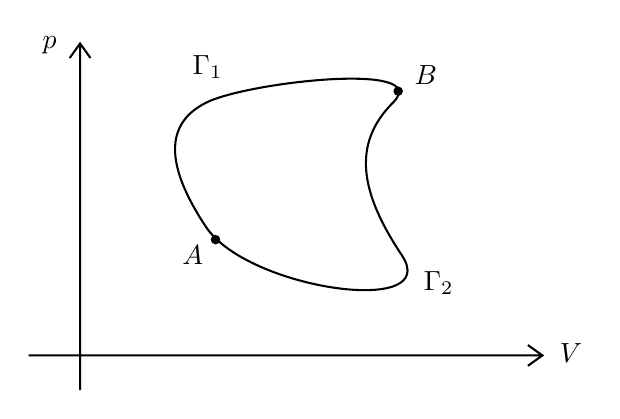
\begin{tikzpicture}[x=0.75pt,y=0.75pt,yscale=-1,xscale=1]
	%uncomment if require: \path (0,300); %set diagram left start at 0, and has height of 300

	%Shape: Axis 2D [id:dp1802588386155528] 
	\draw  (70,222.3) -- (317.5,222.3)(94.75,72) -- (94.75,239) (310.5,217.3) -- (317.5,222.3) -- (310.5,227.3) (89.75,79) -- (94.75,72) -- (99.75,79)  ;
	%Shape: Polygon Curved [id:ds7126263079707398] 
	\draw   (155.5,100.5) .. controls (175.5,90.5) and (265.5,80.5) .. (245.5,100.5) .. controls (225.5,120.5) and (229.75,144) .. (249.75,174) .. controls (269.75,204) and (175.5,190.5) .. (155.5,160.5) .. controls (135.5,130.5) and (135.5,110.5) .. (155.5,100.5) -- cycle ;
	%Shape: Circle [id:dp18230697087752912] 
	\draw  [fill={rgb, 255:red, 0; green, 0; blue, 0 }  ,fill opacity=1 ] (158.25,166.5) .. controls (158.25,165.53) and (159.03,164.75) .. (160,164.75) .. controls (160.97,164.75) and (161.75,165.53) .. (161.75,166.5) .. controls (161.75,167.47) and (160.97,168.25) .. (160,168.25) .. controls (159.03,168.25) and (158.25,167.47) .. (158.25,166.5) -- cycle ;
	%Shape: Circle [id:dp9179639156116408] 
	\draw  [fill={rgb, 255:red, 0; green, 0; blue, 0 }  ,fill opacity=1 ] (246.25,95) .. controls (246.25,94.03) and (247.03,93.25) .. (248,93.25) .. controls (248.97,93.25) and (249.75,94.03) .. (249.75,95) .. controls (249.75,95.97) and (248.97,96.75) .. (248,96.75) .. controls (247.03,96.75) and (246.25,95.97) .. (246.25,95) -- cycle ;

	% Text Node
	\draw (80,73) node    {$p$};
	% Text Node
	\draw (331.33,221.33) node    {$V$};
	% Text Node
	\draw (149,174) node    {$A$};
	% Text Node
	\draw (261.33,87.33) node    {$B$};
	% Text Node
	\draw (156.17,83.33) node    {$\Gamma _{1}$};
	% Text Node
	\draw (267.5,187.33) node    {$\Gamma _{2}$};

	\end{tikzpicture}
\end{figure}
\FloatBarrier
È un ciclo reversibile, per cui si può imporre la validità dell'uguaglianza di Clausius:

\[
	\int_{\Gamma_1, A\to B} \frac{dQ_{\text{rev} } }{T} + \int_{\Gamma_2, B\to A} \frac{dQ_{\text{rev} } }{T} = 0
\]

Poiché la trasformazione $\Gamma_2$ è reversibile, è possibile ribaltarla cambiandone il segno. Sono state realizzate così due trasformazioni diverse che partono dallo stesso stato $A$ iniziale e arrivano allo stesso stato $B$ finale.

\[
	\int_{\Gamma_1, A\to B} \frac{dQ_{\text{rev} } }{T} - \int_{-\Gamma_2, A\to B} \frac{dQ_{\text{rev} } }{T} = 0
\]

Allora:

\[
	\int_{\Gamma_1, A\to B} \frac{dQ_{\text{rev} } }{T} = \int_{-\Gamma_2, A\to B} \frac{dQ_{\text{rev} } }{T}
\]

Quindi date due trasformazioni diverse aventi stato iniziale e finale in comune, la quantità $\int dQ_\text{rev}/T$ è esattamente la stessa. Questo significa che essa non dipende dal particolare percorso, ma solo dallo stato iniziale e finale. Analogamente a quanto visto per l'energia potenziale, esiste allora sempre una funzione scalare, dello stato termodinamico in cui si trova il sistema, che dimensionalmente avrà la dimensione di un'energia su una temperatura, tale per cui:

\[
	\int_A^B \frac{dQ_{\text{rev} } }{T} = f(B) - f(A)
\]

A questa particolare funzione di stato viene dato il nome di \textbf{entropia} e là si indica con la lettera $S$.
La grandezza entropia è una funzione di stato esattamente come lo è l'energia interna di un certo sistema termodinamico, è definita a meno di una costante additiva, ma non ha importanza perché si è interessati alla sua variazione.

\[
	S(p,V,T,n) \quad \text{funzione di stato}
\]

Se si va da uno stato $A$ ad uno stato $B$ con una trasformazione irreversibile, si può comunque usare la definizione di entropia. $\Delta S$ sarà lo stesso di quello che si ottiene quando si fa una trasformazione reversibile. Si prende una qualunque trasformazione che porta da $A$ a $B$ e si considera il calore scambiato il maniera reversibile.

\[
	\int_A^B \frac{dQ_{\text{rev} } }{T} = S(B) - S(A)
\]

\paragraph{$\Delta S$ per una massa che varia temperatura} Si immagini di avere una certa massa caratterizzata dal calore specifico $c$ che inizialmente si trova alla temperatura $T_1$ e che, per contatto termico con un altro corpo, viene scaldata o raffreddata fino ad arrivare alla temperatura $T_2$. Si deve valutare la variazione di entropia di questo sistema termodinamico. Il processo è irreversibile, non passa per continui stati di equilibrio.

\begin{figure}[htpb]
	\centering

	\tikzset{every picture/.style={line width=0.75pt}} %set default line width to 0.75pt        

	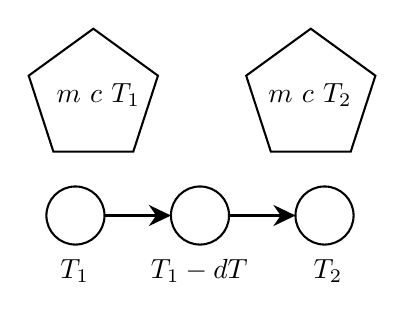
\begin{tikzpicture}[x=0.75pt,y=0.75pt,yscale=-1,xscale=1]
	%uncomment if require: \path (0,300); %set diagram left start at 0, and has height of 300

	%Shape: Polygon [id:dp12394600880731876] 
	\draw   (142.86,124.23) -- (104.37,124.23) -- (92.48,87.62) -- (123.62,65) -- (154.75,87.62) -- cycle ;
	%Shape: Polygon [id:dp5204589102411801] 
	\draw   (247.63,124.23) -- (209.14,124.23) -- (197.25,87.62) -- (228.38,65) -- (259.52,87.62) -- cycle ;
	%Shape: Circle [id:dp7037865140831645] 
	\draw   (101,155) .. controls (101,147.27) and (107.27,141) .. (115,141) .. controls (122.73,141) and (129,147.27) .. (129,155) .. controls (129,162.73) and (122.73,169) .. (115,169) .. controls (107.27,169) and (101,162.73) .. (101,155) -- cycle ;
	%Shape: Circle [id:dp8431154371971894] 
	\draw   (161,155) .. controls (161,147.27) and (167.27,141) .. (175,141) .. controls (182.73,141) and (189,147.27) .. (189,155) .. controls (189,162.73) and (182.73,169) .. (175,169) .. controls (167.27,169) and (161,162.73) .. (161,155) -- cycle ;
	%Shape: Circle [id:dp8473592675610118] 
	\draw   (221,155) .. controls (221,147.27) and (227.27,141) .. (235,141) .. controls (242.73,141) and (249,147.27) .. (249,155) .. controls (249,162.73) and (242.73,169) .. (235,169) .. controls (227.27,169) and (221,162.73) .. (221,155) -- cycle ;
	%Straight Lines [id:da7807212811453503] 
	\draw    (129,155) -- (158,155) ;
	\draw [shift={(161,155)}, rotate = 180] [fill={rgb, 255:red, 0; green, 0; blue, 0 }  ][line width=0.08]  [draw opacity=0] (10.72,-5.15) -- (0,0) -- (10.72,5.15) -- (7.12,0) -- cycle    ;
	%Straight Lines [id:da16236224334225202] 
	\draw    (189,155) -- (218,155) ;
	\draw [shift={(221,155)}, rotate = 180] [fill={rgb, 255:red, 0; green, 0; blue, 0 }  ][line width=0.08]  [draw opacity=0] (10.72,-5.15) -- (0,0) -- (10.72,5.15) -- (7.12,0) -- cycle    ;

	% Text Node
	\draw (126,97) node    {$m\ c\ T_{1}$};
	% Text Node
	\draw (228,97) node    {$m\ c\ T_{2}$};
	% Text Node
	\draw (114.67,181.67) node    {$T_{1}$};
	% Text Node
	\draw (174.67,181.67) node    {$T_{1} -dT$};
	% Text Node
	\draw (236.67,181.67) node    {$T_{2}$};

	\end{tikzpicture}
\end{figure}
\FloatBarrier
Per il calcolo della variazione di entropia nelle trasformazioni irreversibili, basta scegliere una qualsiasi trasformazione reversibile che colleghi $A$ e $B$ e applicare a questa la definizione. Il risultato è valido in ogni caso. Si immagina quindi di raffreddare l'acqua mettendola a contatto con serbatoi di calore di temperature molto prossime tra di loro, anche se nella realtà il processo non sta avvenendo in questo modo, che piano piano abbassano la temperatura dell'acqua da $T_1$ a $T_2$.
Mentre si somma in maniera continua tutta la quantità, bisogna valutare cosa accade dallo stato iniziale allo stato finale. Si ottiene:

\begin{gather*}
	\underbrace{S(B) - S(A)}_{\Delta S} = \int_A^B \frac{dQ_{\text{rev} } }{T} = \int_{T_1 }^{T_2 } \frac{mcdT}{T} = mc\,\log \frac{T_2 }{T_1 } \\
	\Delta S \left\{ \begin{array}{r}
		>0 \quad \text{se} \quad T_2>T_1 \\
		<0 \quad \text{se} \quad T_2<T_1
	\end{array} \right.
\end{gather*}

Si noti che l'integrale non è il calore scambiato dalla massa su $T$.

\[
	Q_{\text{irrev}} = mc\Delta T = mc(T_2-T_1) \neq Q_{\text{rev}}
\]

\paragraph{$\Delta S$ per un serbatoio} Si supponga che la massa inizialmente alla temperatura $T_1$ sia stata portata a temperatura $T_2$ mettendola a contatto con un serbatoio freddo, che va ad assorbire calore dalla massa.

\begin{figure}[htpb]
	\centering

	\tikzset{every picture/.style={line width=0.75pt}} %set default line width to 0.75pt        

	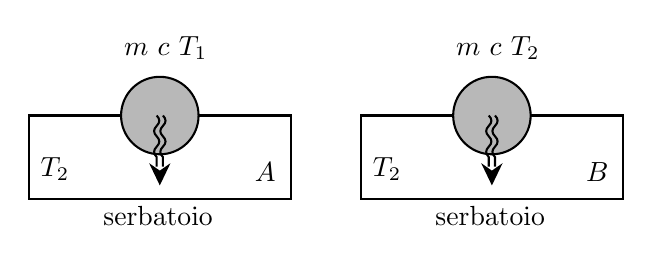
\begin{tikzpicture}[x=0.75pt,y=0.75pt,yscale=-1,xscale=1]
	%uncomment if require: \path (0,300); %set diagram left start at 0, and has height of 300

	%Shape: Rectangle [id:dp7163828634385068] 
	\draw   (110.67,72.33) -- (237,72.33) -- (237,112.33) -- (110.67,112.33) -- cycle ;
	%Shape: Circle [id:dp38214896965195333] 
	\draw  [fill={rgb, 255:red, 184; green, 184; blue, 184 }  ,fill opacity=1 ] (155.17,72.33) .. controls (155.17,62.02) and (163.52,53.67) .. (173.83,53.67) .. controls (184.14,53.67) and (192.5,62.02) .. (192.5,72.33) .. controls (192.5,82.64) and (184.14,91) .. (173.83,91) .. controls (163.52,91) and (155.17,82.64) .. (155.17,72.33) -- cycle ;
	%Straight Lines [id:da7561408389051725] 
	\draw    (175.33,72.33) .. controls (177,74) and (177,75.66) .. (175.33,77.33) .. controls (173.66,79) and (173.66,80.66) .. (175.33,82.33) .. controls (177,84) and (177,85.66) .. (175.33,87.33) .. controls (173.66,89) and (173.66,90.66) .. (175.33,92.33) -- (175.33,94) -- (175.33,97)(172.33,72.33) .. controls (174,74) and (174,75.66) .. (172.33,77.33) .. controls (170.66,79) and (170.66,80.66) .. (172.33,82.33) .. controls (174,84) and (174,85.66) .. (172.33,87.33) .. controls (170.66,89) and (170.66,90.66) .. (172.33,92.33) -- (172.33,94) -- (172.33,97) ;
	\draw [shift={(173.83,106)}, rotate = 270] [fill={rgb, 255:red, 0; green, 0; blue, 0 }  ][line width=0.08]  [draw opacity=0] (10.72,-5.15) -- (0,0) -- (10.72,5.15) -- (7.12,0) -- cycle    ;
	%Shape: Rectangle [id:dp40895364106028165] 
	\draw   (270.67,72.33) -- (397,72.33) -- (397,112.33) -- (270.67,112.33) -- cycle ;
	%Shape: Circle [id:dp18749112210277175] 
	\draw  [fill={rgb, 255:red, 184; green, 184; blue, 184 }  ,fill opacity=1 ] (315.17,72.33) .. controls (315.17,62.02) and (323.52,53.67) .. (333.83,53.67) .. controls (344.14,53.67) and (352.5,62.02) .. (352.5,72.33) .. controls (352.5,82.64) and (344.14,91) .. (333.83,91) .. controls (323.52,91) and (315.17,82.64) .. (315.17,72.33) -- cycle ;
	%Straight Lines [id:da3176905019687204] 
	\draw    (335.33,72.33) .. controls (337,74) and (337,75.66) .. (335.33,77.33) .. controls (333.66,79) and (333.66,80.66) .. (335.33,82.33) .. controls (337,84) and (337,85.66) .. (335.33,87.33) .. controls (333.66,89) and (333.66,90.66) .. (335.33,92.33) -- (335.33,94) -- (335.33,97)(332.33,72.33) .. controls (334,74) and (334,75.66) .. (332.33,77.33) .. controls (330.66,79) and (330.66,80.66) .. (332.33,82.33) .. controls (334,84) and (334,85.66) .. (332.33,87.33) .. controls (330.66,89) and (330.66,90.66) .. (332.33,92.33) -- (332.33,94) -- (332.33,97) ;
	\draw [shift={(333.83,106)}, rotate = 270] [fill={rgb, 255:red, 0; green, 0; blue, 0 }  ][line width=0.08]  [draw opacity=0] (10.72,-5.15) -- (0,0) -- (10.72,5.15) -- (7.12,0) -- cycle    ;

	% Text Node
	\draw (173,120.67) node   [align=left] {serbatoio};
	% Text Node
	\draw (224.67,99.33) node    {$A$};
	% Text Node
	\draw (176.67,40) node    {$m\ c\ T_{1}$};
	% Text Node
	\draw (123.33,98) node    {$T_{2}$};
	% Text Node
	\draw (333,120.67) node   [align=left] {serbatoio};
	% Text Node
	\draw (384.67,99.33) node    {$B$};
	% Text Node
	\draw (336.67,40) node    {$m\ c\ T_{2}$};
	% Text Node
	\draw (283.33,98) node    {$T_{2}$};

	\end{tikzpicture}
\end{figure}
\FloatBarrier
Si calcola la variazione di entropia \emph{del serbatoio} mentre $m$ passa da questo stato iniziale a questo stato finale. Esso assorbe calore dalla massa molto rapidamente, quindi non in maniera reversibile. Quello che si può fare è immaginare di fare avvenire il processo molto lentamente. Questa volta però esso rimane alla temperatura $T_2$.

\[
	\Delta S_{\text{serbatoio}} = \int_A^B \frac{dQ_{\text{rev}} }{T_2} = \frac{\int_A^B dQ_{\text{rev} } }{T_2 } = \frac{Q_{\text{ass, serb }2 } }{T_2}
\]

Il calore assorbito è esattamente quello ceduto dalla massa: $mc\Delta T$. Per i serbatoi, la variazione di entropia è sempre il calore scambiato fratto la temperatura a cui opera, perché essa è costante.

Si immagini di avere questo esempio in cui il serbatoio assorbe calore e quindi esso aumenta la sua entropia.

\[
	\Delta S_{\text{serb} } = \frac{mc(T_1-T_2)}{T_2}
\]

Una parte del sistema aumenta la sua entropia, l'altra parte la diminuisce perché $T_1>T_2$. Le due variazioni di entropia non sono uguali. In un caso è $mc\log(T_2/T_1)$, nell'altro $mc\Delta T$. In realtà si arriverà a dire che se il processo è irreversibile, la variazione netta di entropia di tutte le parti del sistema è sempre positiva.

\[
	\frac{mc(T_1-T_2  )}{T_2 } \neq mc\,\log \frac{T_2 }{T_1}
\]

\paragraph{ $\Delta S$ di un gas perfetto} Si calcoli la variazione di entropia di un gas perfetto che esegue una trasformazione dallo stato $A$ allo stato $B$. Esso sarà caratterizzato da un certo numero di moli. Non bisogna specificare quale trasformazione segue, nè se è reversibile o meno. Si trova $\Delta S$ partendo dalla definizione.

\[
	\Delta S_{\text{gas} } = \int_A^B \frac{dQ_{\text{rev} } }{T}
\]

Utilizzando il primo principio della termodinamica, si può scrivere la variazione infinitesima di lavoro scambiato in maniera reversibile:

\[
	dQ_{\text{rev} } = dU + d\mathcal{L}_{\text{rev} }
\]

Bisogna immaginare che questa piccola trasformazione sia reversibile. Per l'energia interna non va specificato niente perché è una funzione di stato, ma per il lavoro bisogna sottolineare il fatto che si tratta di lavoro fatto in maniera reversibile.

\begin{equation*}
	\begin{aligned}
		\Delta S_{\text{gas} } &= \int_A^B \frac{dU + d\mathcal{L}_{\text{rev} } }{T} \\
		&= \int_A^B \frac{nc_v dT }{T} + \int_A^B \frac{\overbrace{d\mathcal{L}_{\text{rev} }}^{p_{\text{gas}}dV } }{T} \\
		&= \int_A^B \frac{nc_v dT }{T} + \int_A^B \frac{nRT/V}{T}dV \\
		&= \int_A^B \frac{nc_v dT }{T} + \int_A^B \frac{nR}{V}dV \\
		&=nc_v\log \frac{T_B }{T_A } + nR\log \frac{V_B }{V_A }
	\end{aligned}
\end{equation*}

Questa è la relazione che si può utilizzare sempre per calcolare la variazione di entropia di un gas perfetto, qualunque sia la trasformazione che segue.

\[
	\boxed{\Delta S_{\text{gas} } = nc_v\log \frac{T_B }{T_A } + nR\log \frac{V_B }{V_A }}
\]

La si applica a un caso particolare. Si consideri l'esperimento di espansione libera di un gas nel vuoto.

\begin{figure}[htpb]
	\centering

	\tikzset{every picture/.style={line width=0.75pt}} %set default line width to 0.75pt        

	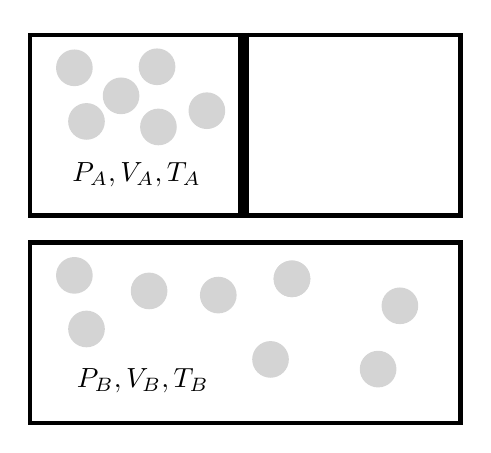
\begin{tikzpicture}[x=0.75pt,y=0.75pt,yscale=-1,xscale=1]
	%uncomment if require: \path (0,300); %set diagram left start at 0, and has height of 300

	%Shape: Rectangle [id:dp7654859373784995] 
	\draw  [line width=1.5]  (132,71) -- (339.5,71) -- (339.5,158) -- (132,158) -- cycle ;
	%Straight Lines [id:da7473689178219229] 
	\draw [line width=3.75]    (235,70) -- (235,158) ;
	%Shape: Circle [id:dp23688450455889987] 
	\draw  [draw opacity=0][fill={rgb, 255:red, 212; green, 212; blue, 212 }  ,fill opacity=1 ] (144.67,86.83) .. controls (144.67,81.95) and (148.62,78) .. (153.5,78) .. controls (158.38,78) and (162.33,81.95) .. (162.33,86.83) .. controls (162.33,91.71) and (158.38,95.67) .. (153.5,95.67) .. controls (148.62,95.67) and (144.67,91.71) .. (144.67,86.83) -- cycle ;
	%Shape: Circle [id:dp22326990723298756] 
	\draw  [draw opacity=0][fill={rgb, 255:red, 212; green, 212; blue, 212 }  ,fill opacity=1 ] (184.5,86.33) .. controls (184.5,81.45) and (188.45,77.5) .. (193.33,77.5) .. controls (198.21,77.5) and (202.17,81.45) .. (202.17,86.33) .. controls (202.17,91.21) and (198.21,95.17) .. (193.33,95.17) .. controls (188.45,95.17) and (184.5,91.21) .. (184.5,86.33) -- cycle ;
	%Shape: Circle [id:dp39356421779783557] 
	\draw  [draw opacity=0][fill={rgb, 255:red, 212; green, 212; blue, 212 }  ,fill opacity=1 ] (208.5,107.5) .. controls (208.5,102.62) and (212.45,98.67) .. (217.33,98.67) .. controls (222.21,98.67) and (226.17,102.62) .. (226.17,107.5) .. controls (226.17,112.38) and (222.21,116.33) .. (217.33,116.33) .. controls (212.45,116.33) and (208.5,112.38) .. (208.5,107.5) -- cycle ;
	%Shape: Circle [id:dp9732115257870197] 
	\draw  [draw opacity=0][fill={rgb, 255:red, 212; green, 212; blue, 212 }  ,fill opacity=1 ] (150.5,112.67) .. controls (150.5,107.79) and (154.45,103.83) .. (159.33,103.83) .. controls (164.21,103.83) and (168.17,107.79) .. (168.17,112.67) .. controls (168.17,117.55) and (164.21,121.5) .. (159.33,121.5) .. controls (154.45,121.5) and (150.5,117.55) .. (150.5,112.67) -- cycle ;
	%Shape: Circle [id:dp14464327361910723] 
	\draw  [draw opacity=0][fill={rgb, 255:red, 212; green, 212; blue, 212 }  ,fill opacity=1 ] (167.17,100.33) .. controls (167.17,95.45) and (171.12,91.5) .. (176,91.5) .. controls (180.88,91.5) and (184.83,95.45) .. (184.83,100.33) .. controls (184.83,105.21) and (180.88,109.17) .. (176,109.17) .. controls (171.12,109.17) and (167.17,105.21) .. (167.17,100.33) -- cycle ;
	%Shape: Circle [id:dp6435399617117978] 
	\draw  [draw opacity=0][fill={rgb, 255:red, 212; green, 212; blue, 212 }  ,fill opacity=1 ] (185.17,115.33) .. controls (185.17,110.45) and (189.12,106.5) .. (194,106.5) .. controls (198.88,106.5) and (202.83,110.45) .. (202.83,115.33) .. controls (202.83,120.21) and (198.88,124.17) .. (194,124.17) .. controls (189.12,124.17) and (185.17,120.21) .. (185.17,115.33) -- cycle ;
	%Shape: Rectangle [id:dp9352467576178161] 
	\draw  [line width=1.5]  (132,171) -- (339.5,171) -- (339.5,258) -- (132,258) -- cycle ;
	%Shape: Circle [id:dp7581647083942251] 
	\draw  [draw opacity=0][fill={rgb, 255:red, 212; green, 212; blue, 212 }  ,fill opacity=1 ] (144.67,186.83) .. controls (144.67,181.95) and (148.62,178) .. (153.5,178) .. controls (158.38,178) and (162.33,181.95) .. (162.33,186.83) .. controls (162.33,191.71) and (158.38,195.67) .. (153.5,195.67) .. controls (148.62,195.67) and (144.67,191.71) .. (144.67,186.83) -- cycle ;
	%Shape: Circle [id:dp11922850645820748] 
	\draw  [draw opacity=0][fill={rgb, 255:red, 212; green, 212; blue, 212 }  ,fill opacity=1 ] (214,196.33) .. controls (214,191.45) and (217.95,187.5) .. (222.83,187.5) .. controls (227.71,187.5) and (231.67,191.45) .. (231.67,196.33) .. controls (231.67,201.21) and (227.71,205.17) .. (222.83,205.17) .. controls (217.95,205.17) and (214,201.21) .. (214,196.33) -- cycle ;
	%Shape: Circle [id:dp8219713042454879] 
	\draw  [draw opacity=0][fill={rgb, 255:red, 212; green, 212; blue, 212 }  ,fill opacity=1 ] (291,232) .. controls (291,227.12) and (294.95,223.17) .. (299.83,223.17) .. controls (304.71,223.17) and (308.67,227.12) .. (308.67,232) .. controls (308.67,236.88) and (304.71,240.83) .. (299.83,240.83) .. controls (294.95,240.83) and (291,236.88) .. (291,232) -- cycle ;
	%Shape: Circle [id:dp9516039190152856] 
	\draw  [draw opacity=0][fill={rgb, 255:red, 212; green, 212; blue, 212 }  ,fill opacity=1 ] (150.5,212.67) .. controls (150.5,207.79) and (154.45,203.83) .. (159.33,203.83) .. controls (164.21,203.83) and (168.17,207.79) .. (168.17,212.67) .. controls (168.17,217.55) and (164.21,221.5) .. (159.33,221.5) .. controls (154.45,221.5) and (150.5,217.55) .. (150.5,212.67) -- cycle ;
	%Shape: Circle [id:dp20810462008863717] 
	\draw  [draw opacity=0][fill={rgb, 255:red, 212; green, 212; blue, 212 }  ,fill opacity=1 ] (180.67,194.33) .. controls (180.67,189.45) and (184.62,185.5) .. (189.5,185.5) .. controls (194.38,185.5) and (198.33,189.45) .. (198.33,194.33) .. controls (198.33,199.21) and (194.38,203.17) .. (189.5,203.17) .. controls (184.62,203.17) and (180.67,199.21) .. (180.67,194.33) -- cycle ;
	%Shape: Circle [id:dp2765007615428927] 
	\draw  [draw opacity=0][fill={rgb, 255:red, 212; green, 212; blue, 212 }  ,fill opacity=1 ] (239.17,227.33) .. controls (239.17,222.45) and (243.12,218.5) .. (248,218.5) .. controls (252.88,218.5) and (256.83,222.45) .. (256.83,227.33) .. controls (256.83,232.21) and (252.88,236.17) .. (248,236.17) .. controls (243.12,236.17) and (239.17,232.21) .. (239.17,227.33) -- cycle ;
	%Shape: Circle [id:dp7090074746213548] 
	\draw  [draw opacity=0][fill={rgb, 255:red, 212; green, 212; blue, 212 }  ,fill opacity=1 ] (301.5,201.5) .. controls (301.5,196.62) and (305.45,192.67) .. (310.33,192.67) .. controls (315.21,192.67) and (319.17,196.62) .. (319.17,201.5) .. controls (319.17,206.38) and (315.21,210.33) .. (310.33,210.33) .. controls (305.45,210.33) and (301.5,206.38) .. (301.5,201.5) -- cycle ;
	%Shape: Circle [id:dp32636661863574723] 
	\draw  [draw opacity=0][fill={rgb, 255:red, 212; green, 212; blue, 212 }  ,fill opacity=1 ] (249.5,188.5) .. controls (249.5,183.62) and (253.45,179.67) .. (258.33,179.67) .. controls (263.21,179.67) and (267.17,183.62) .. (267.17,188.5) .. controls (267.17,193.38) and (263.21,197.33) .. (258.33,197.33) .. controls (253.45,197.33) and (249.5,193.38) .. (249.5,188.5) -- cycle ;
	%Shape: Circle [id:dp35918471123787743] 
	\draw  [draw opacity=0][fill={rgb, 255:red, 212; green, 212; blue, 212 }  ,fill opacity=1 ] (249.5,188.5) .. controls (249.5,183.62) and (253.45,179.67) .. (258.33,179.67) .. controls (263.21,179.67) and (267.17,183.62) .. (267.17,188.5) .. controls (267.17,193.38) and (263.21,197.33) .. (258.33,197.33) .. controls (253.45,197.33) and (249.5,193.38) .. (249.5,188.5) -- cycle ;

	% Text Node
	\draw (183.5,138.5) node    {$P_{A} ,V_{A} ,T_{A}$};
	% Text Node
	\draw (186.5,237.5) node    {$P_{B} ,V_{B} ,T_{B}$};

	\end{tikzpicture}
\end{figure}
\FloatBarrier
Si tratta di un processo irreversibile, il gas non tornerà mai indietro. Si tratta di un'espansione adiabatica. Visto che il gas non scambia calore, si potrebbe pensare che allora nella relazione $dQ$ è pari a $0$ e quindi la variazione di entropia è nulla. Il calore scambiato invece non lo si può usare per calcolare la variazione di entropia perché è quello scambiato in maniera irreversibile. Per questo specifico caso, usando invece la relazione appena trovata:

\[
	nc_v\log \frac{T_B }{T_A } = 0 \implies \Delta S_{\text{gas} } = nR\log \frac{V_B }{V_A }
\]

In questo caso il gas aumenta sempre la sua entropia.

\paragraph{Osservazione} L'entropia può essere scritta anche in forma infinitesima, con riferimento ad una trasformazione reversibile infinitesima, che implica una variazione infinitesima delle coordinate termodinamiche:

\[
	dS = \left( \frac{dQ}{T} \right)_{\text{rev}}
\]
$dQ$ non è un differenziale esatto però se tale quantità è divisa per $T$ ed è considerata in una trasformazione reversibile, essa dà luogo al differenziale esatto $dS$.

\section{Principio di accrescimento dell'entropia dell'universo}

Si vede ora quali informazioni in più porta considerare la disuguaglianza di Clausius con il segno di minore stretto.  Per capirlo, si ripete la stessa dimostrazione che ha portato a definire l'entropia. Si consideri l'integrale definito per un ciclo. Tale ciclo è irreversibile, in particolare, si fa in modo che esso possa essere spezzato in due parti $A$ e $B$, tali per cui $AB$ è irreversibile, mentre $BA$ è reversibile.

\begin{figure}[htpb]
	\centering

	\tikzset{every picture/.style={line width=0.75pt}} %set default line width to 0.75pt        

	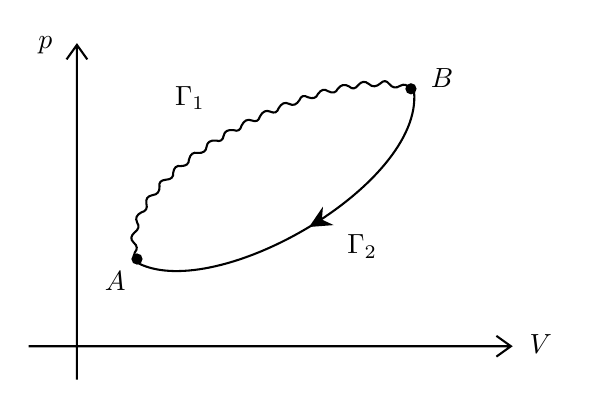
\begin{tikzpicture}[x=0.75pt,y=0.75pt,yscale=-1,xscale=1]
	%uncomment if require: \path (0,300); %set diagram left start at 0, and has height of 300

	%Shape: Axis 2D [id:dp5387427598927963] 
	\draw  (70,229.2) -- (302.33,229.2)(93.23,84) -- (93.23,245.33) (295.33,224.2) -- (302.33,229.2) -- (295.33,234.2) (88.23,91) -- (93.23,84) -- (98.23,91)  ;
	%Curve Lines [id:da06279909715521925] 
	\draw    (123,189.33) .. controls (120.69,188.11) and (120.06,186.33) .. (121.13,183.99) .. controls (122.54,182.42) and (122.36,180.83) .. (120.57,179.23) .. controls (118.94,177.74) and (119.07,176.14) .. (120.96,174.41) .. controls (122.98,173) and (123.4,171.38) .. (122.23,169.55) .. controls (121.22,167.52) and (121.92,165.9) .. (124.32,164.69) .. controls (126.51,164.14) and (127.31,162.75) .. (126.71,160.54) .. controls (126.28,158.2) and (127.25,156.82) .. (129.62,156.41) .. controls (131.99,156.11) and (133.12,154.75) .. (133.01,152.32) .. controls (132.6,150.29) and (133.65,149.17) .. (136.16,148.96) .. controls (138.67,148.83) and (139.81,147.73) .. (139.6,145.65) .. controls (139.97,143.08) and (141.2,142) .. (143.3,142.39) .. controls (145.9,142.4) and (147.21,141.34) .. (147.23,139.2) .. controls (147.88,136.61) and (149.26,135.57) .. (151.37,136.08) .. controls (154.04,136.23) and (155.49,135.22) .. (155.71,133.05) .. controls (155.98,130.86) and (157.48,129.88) .. (160.21,130.1) .. controls (162.31,130.75) and (163.54,129.99) .. (163.91,127.82) .. controls (164.33,125.64) and (165.91,124.72) .. (168.66,125.07) .. controls (170.74,125.82) and (172.03,125.11) .. (172.53,122.95) .. controls (173.72,120.44) and (175.36,119.6) .. (177.44,120.41) .. controls (179.49,121.26) and (180.82,120.61) .. (181.41,118.48) .. controls (182.72,116.03) and (184.39,115.27) .. (186.42,116.18) .. controls (188.42,117.13) and (189.76,116.55) .. (190.44,114.45) .. controls (191.83,112.08) and (193.51,111.41) .. (195.47,112.43) .. controls (197.39,113.48) and (199.06,112.86) .. (200.47,110.57) .. controls (201.26,108.53) and (202.59,108.08) .. (204.45,109.21) .. controls (206.92,110.17) and (208.55,109.66) .. (209.36,107.67) .. controls (210.86,105.51) and (212.47,105.06) .. (214.19,106.32) .. controls (216.48,107.46) and (218.06,107.07) .. (218.91,105.16) .. controls (220.43,103.13) and (222.26,102.76) .. (224.41,104.05) .. controls (225.86,105.5) and (227.33,105.27) .. (228.81,103.36) .. controls (230.34,101.5) and (232.03,101.32) .. (233.86,102.83) .. controls (235.54,104.4) and (237.38,104.34) .. (239.37,102.64) .. controls (240.94,101.02) and (242.39,101.09) .. (243.72,102.86) .. controls (245.24,104.74) and (246.97,105.03) .. (248.92,103.74) .. controls (251.02,102.63) and (252.49,103.16) .. (253.34,105.31) -- (255.67,106.67) ;
	%Curve Lines [id:da995829034171916] 
	\draw    (123,189.33) .. controls (161,208) and (259.67,151.33) .. (255.67,106.67) ;
	\draw [shift={(205.08,171.75)}, rotate = 329.9] [fill={rgb, 255:red, 0; green, 0; blue, 0 }  ][line width=0.08]  [draw opacity=0] (10.72,-5.15) -- (0,0) -- (10.72,5.15) -- (7.12,0) -- cycle    ;
	%Shape: Circle [id:dp006572357997259193] 
	\draw  [fill={rgb, 255:red, 0; green, 0; blue, 0 }  ,fill opacity=1 ] (120,187.17) .. controls (120,185.97) and (120.97,185) .. (122.17,185) .. controls (123.36,185) and (124.33,185.97) .. (124.33,187.17) .. controls (124.33,188.36) and (123.36,189.33) .. (122.17,189.33) .. controls (120.97,189.33) and (120,188.36) .. (120,187.17) -- cycle ;
	%Shape: Circle [id:dp7516795691016311] 
	\draw  [fill={rgb, 255:red, 0; green, 0; blue, 0 }  ,fill opacity=1 ] (252,105.17) .. controls (252,103.97) and (252.97,103) .. (254.17,103) .. controls (255.36,103) and (256.33,103.97) .. (256.33,105.17) .. controls (256.33,106.36) and (255.36,107.33) .. (254.17,107.33) .. controls (252.97,107.33) and (252,106.36) .. (252,105.17) -- cycle ;

	% Text Node
	\draw (78,84.33) node    {$p$};
	% Text Node
	\draw (316.67,228.33) node    {$V$};
	% Text Node
	\draw (111.67,197.67) node    {$A$};
	% Text Node
	\draw (269.17,100.17) node    {$B$};
	% Text Node
	\draw (147.67,109.67) node    {$\Gamma_{1}$};
	% Text Node
	\draw (230.67,181.17) node    {$\Gamma_{2}$};

	\end{tikzpicture}
\end{figure}
\FloatBarrier

\[
	\oint \frac{dQ_{\text{rev} } }{T} = \int_{\Gamma_1,A\to B } \frac{dQ_{\text{irr} } }{T} + \underbrace{\int_{\Gamma_2,B\to A} \frac{dQ_{\text{rev} } }{T}}_{S(A)-S(B)} < 0
\]

La quantità a secondo termine non è altro che la variazione di entropia da $B$ ad $A$. Si sposta a destra $S(A)-S(B)$ cambiandolo di segno.

\[
	\int_{\Gamma_1,A\to B } \frac{dQ_{\text{irr} } }{T} < S(B)-S(A)
\]

Considerati uno stato iniziale $A$ e uno stato finale $B$, se si valuta la variazione di entropia fra questi due stati, quella che si misura è maggiore della somma continua del calore scambiato in maniera irreversibile su $T$.

\[
	S(B)-S(A) > \int_{\Gamma_1,A\to B } \frac{dQ_{\text{irr} } }{T}
\]

Si applica questo risultato alla valutazione della variazione di entropia di un sistema isolato. Si è visto che il sistema termodinamico entra in contatto con un ambiente circostante. In generale esso cede o assorbe calore dall'ambiente circostante. Il complesso sistema termodinamico-ambiente circostante viene detto universo termodinamico. Fondamentalmente gli scambi di calore e di lavoro sono pensati solo fra il sistema termodinamico e l'ambiente. Non c'è altro calore che esce fuori. È come se si immaginasse l'ambiente chiuso in un contenitore adiabatico. Per l'universo termodinamico si può fare una affermazione in termini di calore scambiato: esso è sempre uguale a $0$. C'è solo passaggio di calore fra sistema e l'ambiente ma non esce nulla fuori. Si applicano queste considerazioni ottenute al caso in cui si valuta ciò che accade per l'intero universo termodinamico. Si vuole capire quanto vale la variazione di entropia dell'universo.

\[
	\Delta S_{\text{universo} } = \int_A^B \frac{dQ_{\text{rev} } }{T}
\]

Se all'interno dell'universo termodinamico avvengono solo trasformazioni reversibili il calore totale scambiato è quello reversibile. Dal momento che l'universo è isolato, il secondo termine vale $0$ perché tutte le trasformazioni nell'ipotesi sono reversibili. Ciò significa che in questo caso la variazione di entropia sarà quindi uguale a $0$ e l'entropia è costante. Non aumenta quando si fa passare il sistema da uno stato iniziale a un altro stato.

\[
	\Delta S_{\text{universo}} = S(B)-S(A) > \int \frac{dQ_{\text{irr} } }{T}
\]

Se invece nell'universo avvengono anche trasformazioni irreversibili, chi va a $0$ è il termine $dQ_\text{irr}/T$. Quando ci sono trasformazioni irreversibili, l'entropia dell'universo non può che aumentare. Questo risultato prende il nome di \text{principio di accrescimento dell'entropia dell'universo}. Esso fondamentalmente afferma che se si prende un universo termodinamico, o equivalentemente un sistema isolato dal resto del mondo,  quando esso passa da stato iniziale a stato finale, la variazione di entropia che subisce è sempre maggiore o al limite uguale a zero. L'entropia aumenta se c'è anche solo un processo irreversibile, si mantiene costante solo se tutte le trasformazioni sono reversibili.

\[
	\text{trasformazioni}
	\left\{ \begin{array}{l}
	 	\text{reversibili} \implies \Delta S_{\text{universo}} = 0 \\
		\text{irreversibili} \implies  \Delta S_{\text{universo}} > 0
	\end{array} \right.
\]

Riscrivendo il risultato in maniera più compatta:

\[
	\boxed{\Delta S_{\text{universo}} \geq 0}
\]

Si potrebbe avere una trasformazione in cui per una certa parte del sistema termodinamico l'entropia diminuisce, ma contemporaneamente ci deve essere un'altra parte del sistema per cui l'entropia aumenta. Se il processo è reversibile, la diminuzione di entropia in una certa parte del sistema è bilanciata dall'aumento di entropia di un'altra parte del sistema. Se il processo è irreversibile, chi aumenta l'entropia subirà un aumento maggiore di chi la diminuisce, così che al netto la variazione di entropia è strettamente positiva. Dal punto di vista più generale, il principio lo si può vedere come un altro modo di enunciare il secondo principio della termodinamica. Ci si è arrivati infatti a partire dal teorema di Carnot, dimostrato sfruttando l'enunciato di Clausius del secondo principio della termodinamica.

I processi che avvengono realmente tendono sempre a generare una forma di energia che è più disordinata di quella avuta in partenza. Il principio di accrescimento dell'entropia dell'universo ha il significato di affermare che il disordine dell'universo tende sempre ad aumentare. Si è visto questo anche quando è stato fatto l'esempio dell'oggetto che si muove su un piano. L'energia cinetica ordinata si trasforma spontaneamente in calore, che è un'energia più disordinata legata al moto di agitazione termica delle molecole.

\begin{figure}[htpb]
	\centering

	\tikzset{every picture/.style={line width=0.75pt}} %set default line width to 0.75pt        

	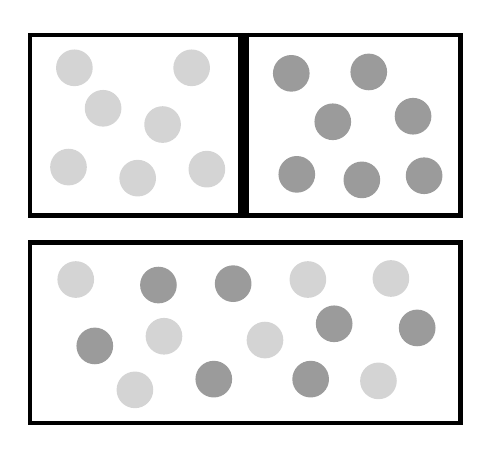
\begin{tikzpicture}[x=0.75pt,y=0.75pt,yscale=-1,xscale=1]
	%uncomment if require: \path (0,300); %set diagram left start at 0, and has height of 300

	%Shape: Rectangle [id:dp1499911640223488] 
	\draw  [line width=1.5]  (132,71) -- (339.5,71) -- (339.5,158) -- (132,158) -- cycle ;
	%Straight Lines [id:da4030620174178323] 
	\draw [line width=3.75]    (235,70) -- (235,158) ;
	%Shape: Circle [id:dp24482697243748608] 
	\draw  [draw opacity=0][fill={rgb, 255:red, 212; green, 212; blue, 212 }  ,fill opacity=1 ] (144.67,86.83) .. controls (144.67,81.95) and (148.62,78) .. (153.5,78) .. controls (158.38,78) and (162.33,81.95) .. (162.33,86.83) .. controls (162.33,91.71) and (158.38,95.67) .. (153.5,95.67) .. controls (148.62,95.67) and (144.67,91.71) .. (144.67,86.83) -- cycle ;
	%Shape: Circle [id:dp5633133397032646] 
	\draw  [draw opacity=0][fill={rgb, 255:red, 212; green, 212; blue, 212 }  ,fill opacity=1 ] (208.5,135.67) .. controls (208.5,130.79) and (212.45,126.83) .. (217.33,126.83) .. controls (222.21,126.83) and (226.17,130.79) .. (226.17,135.67) .. controls (226.17,140.55) and (222.21,144.5) .. (217.33,144.5) .. controls (212.45,144.5) and (208.5,140.55) .. (208.5,135.67) -- cycle ;
	%Shape: Circle [id:dp10481425575013792] 
	\draw  [draw opacity=0][fill={rgb, 255:red, 212; green, 212; blue, 212 }  ,fill opacity=1 ] (187.17,114.17) .. controls (187.17,109.29) and (191.12,105.33) .. (196,105.33) .. controls (200.88,105.33) and (204.83,109.29) .. (204.83,114.17) .. controls (204.83,119.05) and (200.88,123) .. (196,123) .. controls (191.12,123) and (187.17,119.05) .. (187.17,114.17) -- cycle ;
	%Shape: Circle [id:dp46629536046966136] 
	\draw  [draw opacity=0][fill={rgb, 255:red, 212; green, 212; blue, 212 }  ,fill opacity=1 ] (141.83,134.67) .. controls (141.83,129.79) and (145.79,125.83) .. (150.67,125.83) .. controls (155.55,125.83) and (159.5,129.79) .. (159.5,134.67) .. controls (159.5,139.55) and (155.55,143.5) .. (150.67,143.5) .. controls (145.79,143.5) and (141.83,139.55) .. (141.83,134.67) -- cycle ;
	%Shape: Circle [id:dp7346336625541874] 
	\draw  [draw opacity=0][fill={rgb, 255:red, 212; green, 212; blue, 212 }  ,fill opacity=1 ] (158.5,106.33) .. controls (158.5,101.45) and (162.45,97.5) .. (167.33,97.5) .. controls (172.21,97.5) and (176.17,101.45) .. (176.17,106.33) .. controls (176.17,111.21) and (172.21,115.17) .. (167.33,115.17) .. controls (162.45,115.17) and (158.5,111.21) .. (158.5,106.33) -- cycle ;
	%Shape: Circle [id:dp768155105372726] 
	\draw  [draw opacity=0][fill={rgb, 255:red, 212; green, 212; blue, 212 }  ,fill opacity=1 ] (175.17,140) .. controls (175.17,135.12) and (179.12,131.17) .. (184,131.17) .. controls (188.88,131.17) and (192.83,135.12) .. (192.83,140) .. controls (192.83,144.88) and (188.88,148.83) .. (184,148.83) .. controls (179.12,148.83) and (175.17,144.88) .. (175.17,140) -- cycle ;
	%Shape: Rectangle [id:dp4130826075758587] 
	\draw  [line width=1.5]  (132,171) -- (339.5,171) -- (339.5,258) -- (132,258) -- cycle ;
	%Shape: Circle [id:dp2121341951790583] 
	\draw  [draw opacity=0][fill={rgb, 255:red, 212; green, 212; blue, 212 }  ,fill opacity=1 ] (201.17,86.83) .. controls (201.17,81.95) and (205.12,78) .. (210,78) .. controls (214.88,78) and (218.83,81.95) .. (218.83,86.83) .. controls (218.83,91.71) and (214.88,95.67) .. (210,95.67) .. controls (205.12,95.67) and (201.17,91.71) .. (201.17,86.83) -- cycle ;
	%Shape: Circle [id:dp9598242837355548] 
	\draw  [draw opacity=0][fill={rgb, 255:red, 155; green, 155; blue, 155 }  ,fill opacity=1 ] (249.17,89.5) .. controls (249.17,84.62) and (253.12,80.67) .. (258,80.67) .. controls (262.88,80.67) and (266.83,84.62) .. (266.83,89.5) .. controls (266.83,94.38) and (262.88,98.33) .. (258,98.33) .. controls (253.12,98.33) and (249.17,94.38) .. (249.17,89.5) -- cycle ;
	%Shape: Circle [id:dp7914645715580639] 
	\draw  [draw opacity=0][fill={rgb, 255:red, 155; green, 155; blue, 155 }  ,fill opacity=1 ] (286.5,88.83) .. controls (286.5,83.95) and (290.45,80) .. (295.33,80) .. controls (300.21,80) and (304.17,83.95) .. (304.17,88.83) .. controls (304.17,93.71) and (300.21,97.67) .. (295.33,97.67) .. controls (290.45,97.67) and (286.5,93.71) .. (286.5,88.83) -- cycle ;
	%Shape: Circle [id:dp714912835594077] 
	\draw  [draw opacity=0][fill={rgb, 255:red, 155; green, 155; blue, 155 }  ,fill opacity=1 ] (269.17,112.83) .. controls (269.17,107.95) and (273.12,104) .. (278,104) .. controls (282.88,104) and (286.83,107.95) .. (286.83,112.83) .. controls (286.83,117.71) and (282.88,121.67) .. (278,121.67) .. controls (273.12,121.67) and (269.17,117.71) .. (269.17,112.83) -- cycle ;
	%Shape: Circle [id:dp6674219180240206] 
	\draw  [draw opacity=0][fill={rgb, 255:red, 155; green, 155; blue, 155 }  ,fill opacity=1 ] (307.83,110.17) .. controls (307.83,105.29) and (311.79,101.33) .. (316.67,101.33) .. controls (321.55,101.33) and (325.5,105.29) .. (325.5,110.17) .. controls (325.5,115.05) and (321.55,119) .. (316.67,119) .. controls (311.79,119) and (307.83,115.05) .. (307.83,110.17) -- cycle ;
	%Shape: Circle [id:dp38802677325492496] 
	\draw  [draw opacity=0][fill={rgb, 255:red, 155; green, 155; blue, 155 }  ,fill opacity=1 ] (283.17,140.83) .. controls (283.17,135.95) and (287.12,132) .. (292,132) .. controls (296.88,132) and (300.83,135.95) .. (300.83,140.83) .. controls (300.83,145.71) and (296.88,149.67) .. (292,149.67) .. controls (287.12,149.67) and (283.17,145.71) .. (283.17,140.83) -- cycle ;
	%Shape: Circle [id:dp07135425312606158] 
	\draw  [draw opacity=0][fill={rgb, 255:red, 155; green, 155; blue, 155 }  ,fill opacity=1 ] (251.83,138.17) .. controls (251.83,133.29) and (255.79,129.33) .. (260.67,129.33) .. controls (265.55,129.33) and (269.5,133.29) .. (269.5,138.17) .. controls (269.5,143.05) and (265.55,147) .. (260.67,147) .. controls (255.79,147) and (251.83,143.05) .. (251.83,138.17) -- cycle ;
	%Shape: Circle [id:dp28812148833016016] 
	\draw  [draw opacity=0][fill={rgb, 255:red, 155; green, 155; blue, 155 }  ,fill opacity=1 ] (313.17,138.83) .. controls (313.17,133.95) and (317.12,130) .. (322,130) .. controls (326.88,130) and (330.83,133.95) .. (330.83,138.83) .. controls (330.83,143.71) and (326.88,147.67) .. (322,147.67) .. controls (317.12,147.67) and (313.17,143.71) .. (313.17,138.83) -- cycle ;
	%Shape: Circle [id:dp22984044315113872] 
	\draw  [draw opacity=0][fill={rgb, 255:red, 155; green, 155; blue, 155 }  ,fill opacity=1 ] (154.5,220.83) .. controls (154.5,215.95) and (158.45,212) .. (163.33,212) .. controls (168.21,212) and (172.17,215.95) .. (172.17,220.83) .. controls (172.17,225.71) and (168.21,229.67) .. (163.33,229.67) .. controls (158.45,229.67) and (154.5,225.71) .. (154.5,220.83) -- cycle ;
	%Shape: Circle [id:dp5312743164052502] 
	\draw  [draw opacity=0][fill={rgb, 255:red, 155; green, 155; blue, 155 }  ,fill opacity=1 ] (269.83,210.17) .. controls (269.83,205.29) and (273.79,201.33) .. (278.67,201.33) .. controls (283.55,201.33) and (287.5,205.29) .. (287.5,210.17) .. controls (287.5,215.05) and (283.55,219) .. (278.67,219) .. controls (273.79,219) and (269.83,215.05) .. (269.83,210.17) -- cycle ;
	%Shape: Circle [id:dp3499674700441038] 
	\draw  [draw opacity=0][fill={rgb, 255:red, 155; green, 155; blue, 155 }  ,fill opacity=1 ] (185.17,191.5) .. controls (185.17,186.62) and (189.12,182.67) .. (194,182.67) .. controls (198.88,182.67) and (202.83,186.62) .. (202.83,191.5) .. controls (202.83,196.38) and (198.88,200.33) .. (194,200.33) .. controls (189.12,200.33) and (185.17,196.38) .. (185.17,191.5) -- cycle ;
	%Shape: Circle [id:dp8378654755230381] 
	\draw  [draw opacity=0][fill={rgb, 255:red, 155; green, 155; blue, 155 }  ,fill opacity=1 ] (309.83,212.17) .. controls (309.83,207.29) and (313.79,203.33) .. (318.67,203.33) .. controls (323.55,203.33) and (327.5,207.29) .. (327.5,212.17) .. controls (327.5,217.05) and (323.55,221) .. (318.67,221) .. controls (313.79,221) and (309.83,217.05) .. (309.83,212.17) -- cycle ;
	%Shape: Circle [id:dp5028590035257423] 
	\draw  [draw opacity=0][fill={rgb, 255:red, 155; green, 155; blue, 155 }  ,fill opacity=1 ] (258.5,236.83) .. controls (258.5,231.95) and (262.45,228) .. (267.33,228) .. controls (272.21,228) and (276.17,231.95) .. (276.17,236.83) .. controls (276.17,241.71) and (272.21,245.67) .. (267.33,245.67) .. controls (262.45,245.67) and (258.5,241.71) .. (258.5,236.83) -- cycle ;
	%Shape: Circle [id:dp11373845294447271] 
	\draw  [draw opacity=0][fill={rgb, 255:red, 155; green, 155; blue, 155 }  ,fill opacity=1 ] (211.83,236.83) .. controls (211.83,231.95) and (215.79,228) .. (220.67,228) .. controls (225.55,228) and (229.5,231.95) .. (229.5,236.83) .. controls (229.5,241.71) and (225.55,245.67) .. (220.67,245.67) .. controls (215.79,245.67) and (211.83,241.71) .. (211.83,236.83) -- cycle ;
	%Shape: Circle [id:dp621786237948103] 
	\draw  [draw opacity=0][fill={rgb, 255:red, 155; green, 155; blue, 155 }  ,fill opacity=1 ] (221.17,190.83) .. controls (221.17,185.95) and (225.12,182) .. (230,182) .. controls (234.88,182) and (238.83,185.95) .. (238.83,190.83) .. controls (238.83,195.71) and (234.88,199.67) .. (230,199.67) .. controls (225.12,199.67) and (221.17,195.71) .. (221.17,190.83) -- cycle ;
	%Shape: Circle [id:dp10207076001389193] 
	\draw  [draw opacity=0][fill={rgb, 255:red, 212; green, 212; blue, 212 }  ,fill opacity=1 ] (145.33,188.83) .. controls (145.33,183.95) and (149.29,180) .. (154.17,180) .. controls (159.05,180) and (163,183.95) .. (163,188.83) .. controls (163,193.71) and (159.05,197.67) .. (154.17,197.67) .. controls (149.29,197.67) and (145.33,193.71) .. (145.33,188.83) -- cycle ;
	%Shape: Circle [id:dp4968942376874157] 
	\draw  [draw opacity=0][fill={rgb, 255:red, 212; green, 212; blue, 212 }  ,fill opacity=1 ] (291.17,237.67) .. controls (291.17,232.79) and (295.12,228.83) .. (300,228.83) .. controls (304.88,228.83) and (308.83,232.79) .. (308.83,237.67) .. controls (308.83,242.55) and (304.88,246.5) .. (300,246.5) .. controls (295.12,246.5) and (291.17,242.55) .. (291.17,237.67) -- cycle ;
	%Shape: Circle [id:dp3748523271121522] 
	\draw  [draw opacity=0][fill={rgb, 255:red, 212; green, 212; blue, 212 }  ,fill opacity=1 ] (187.83,216.17) .. controls (187.83,211.29) and (191.79,207.33) .. (196.67,207.33) .. controls (201.55,207.33) and (205.5,211.29) .. (205.5,216.17) .. controls (205.5,221.05) and (201.55,225) .. (196.67,225) .. controls (191.79,225) and (187.83,221.05) .. (187.83,216.17) -- cycle ;
	%Shape: Circle [id:dp1434364339701799] 
	\draw  [draw opacity=0][fill={rgb, 255:red, 212; green, 212; blue, 212 }  ,fill opacity=1 ] (173.83,242) .. controls (173.83,237.12) and (177.79,233.17) .. (182.67,233.17) .. controls (187.55,233.17) and (191.5,237.12) .. (191.5,242) .. controls (191.5,246.88) and (187.55,250.83) .. (182.67,250.83) .. controls (177.79,250.83) and (173.83,246.88) .. (173.83,242) -- cycle ;
	%Shape: Circle [id:dp11933510273696224] 
	\draw  [draw opacity=0][fill={rgb, 255:red, 212; green, 212; blue, 212 }  ,fill opacity=1 ] (297.17,188.33) .. controls (297.17,183.45) and (301.12,179.5) .. (306,179.5) .. controls (310.88,179.5) and (314.83,183.45) .. (314.83,188.33) .. controls (314.83,193.21) and (310.88,197.17) .. (306,197.17) .. controls (301.12,197.17) and (297.17,193.21) .. (297.17,188.33) -- cycle ;
	%Shape: Circle [id:dp6178267766318197] 
	\draw  [draw opacity=0][fill={rgb, 255:red, 212; green, 212; blue, 212 }  ,fill opacity=1 ] (236.5,218) .. controls (236.5,213.12) and (240.45,209.17) .. (245.33,209.17) .. controls (250.21,209.17) and (254.17,213.12) .. (254.17,218) .. controls (254.17,222.88) and (250.21,226.83) .. (245.33,226.83) .. controls (240.45,226.83) and (236.5,222.88) .. (236.5,218) -- cycle ;
	%Shape: Circle [id:dp24762806284995897] 
	\draw  [draw opacity=0][fill={rgb, 255:red, 212; green, 212; blue, 212 }  ,fill opacity=1 ] (257.17,188.83) .. controls (257.17,183.95) and (261.12,180) .. (266,180) .. controls (270.88,180) and (274.83,183.95) .. (274.83,188.83) .. controls (274.83,193.71) and (270.88,197.67) .. (266,197.67) .. controls (261.12,197.67) and (257.17,193.71) .. (257.17,188.83) -- cycle ;

	\end{tikzpicture}
\end{figure}
\FloatBarrier
C'è un esempio tipico sul fatto che il disordine molecolare aumenta sempre. Se si prende un contenitore diviso in due parti da una parete, in cui si mettono tante palline rosse da una parte e tante nere dall'altra, inizialmente le due parti del sistema sono molto ordinate. Se ad un certo punto si rimuove la parete e si agita il sistema, spontaneamente accade che le palline si mischiano e la probabilità che tutte le palline di un colore ritornino da una parte e tutte quelle dell'altro nell'altra, è assolutamente nulla. Questa è una visualizzazione del fatto che nell'universo ci sono sempre fenomeni che tendono a portare all'aumento del disordine molecolare, per cui spontaneamente si avrà un suo aumento.

\section{Esempi di calcolo della variazione di entropia di un sistema isolato}

In seguito ci sono alcuni esempi in cui si verifica questo principio calcolando la variazione di entropia dell'universo.

\paragraph{Esempio 1} Si valuta cosa accade quando si ha una macchina termica che sta compiendo un ciclo termodinamico e si calcola la variazione di entropia dell'universo nei due casi in cui il ciclo è percorso in maniera reversibile o irreversibile.

\begin{figure}[htpb]
	\centering

	\tikzset{every picture/.style={line width=0.75pt}} %set default line width to 0.75pt        

	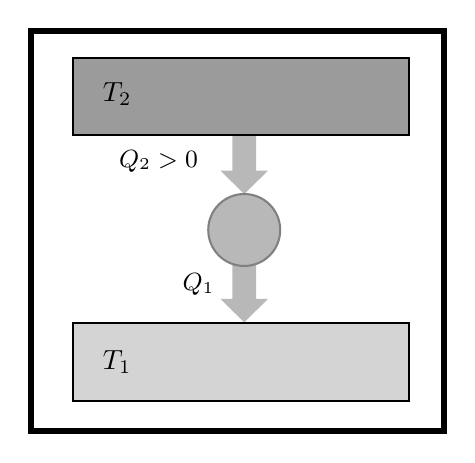
\begin{tikzpicture}[x=0.75pt,y=0.75pt,yscale=-1,xscale=1]
	%uncomment if require: \path (0,300); %set diagram left start at 0, and has height of 300

	%Right Arrow [id:dp29085795084499666] 
	\draw  [draw opacity=0][fill={rgb, 255:red, 184; green, 184; blue, 184 }  ,fill opacity=1 ] (178.06,177.31) -- (178.06,194.19) -- (183.8,194.19) -- (172.33,205.45) -- (160.87,194.19) -- (166.6,194.19) -- (166.6,177.31) -- cycle ;
	%Right Arrow [id:dp3212737354734736] 
	\draw  [draw opacity=0][fill={rgb, 255:red, 184; green, 184; blue, 184 }  ,fill opacity=1 ] (178.06,115.5) -- (178.06,132.38) -- (183.8,132.38) -- (172.33,143.64) -- (160.87,132.38) -- (166.6,132.38) -- (166.6,115.5) -- cycle ;
	%Shape: Rectangle [id:dp5029916281625293] 
	\draw  [fill={rgb, 255:red, 155; green, 155; blue, 155 }  ,fill opacity=1 ] (90,78) -- (251.5,78) -- (251.5,115.27) -- (90,115.27) -- cycle ;
	%Shape: Rectangle [id:dp3067577613932537] 
	\draw  [fill={rgb, 255:red, 212; green, 212; blue, 212 }  ,fill opacity=1 ] (90,205.9) -- (251.5,205.9) -- (251.5,243.17) -- (90,243.17) -- cycle ;
	%Shape: Ellipse [id:dp546617301961033] 
	\draw  [color={rgb, 255:red, 128; green, 128; blue, 128 }  ,draw opacity=1 ][fill={rgb, 255:red, 184; green, 184; blue, 184 }  ,fill opacity=1 ] (155,160.97) .. controls (155,151.4) and (162.76,143.64) .. (172.33,143.64) .. controls (181.91,143.64) and (189.67,151.4) .. (189.67,160.97) .. controls (189.67,170.55) and (181.91,178.31) .. (172.33,178.31) .. controls (162.76,178.31) and (155,170.55) .. (155,160.97) -- cycle ;
	%Shape: Rectangle [id:dp149197922715806] 
	\draw  [line width=2.25]  (69.5,65) -- (268.5,65) -- (268.5,258) -- (69.5,258) -- cycle ;

	% Text Node
	\draw (111.12,95.39) node    {$T_{2}$};
	% Text Node
	\draw (111.12,224.53) node    {$T_{1}$};
	% Text Node
	\draw (131.03,127.7) node  [font=\small]  {$Q_{2}  >0$};
	% Text Node
	\draw (150.33,187.4) node  [font=\small]  {$Q_{1}$};

	\end{tikzpicture}
\end{figure}
\FloatBarrier

\begin{itemize}
	\item Si prova a vedere cosa accade per un ciclo di Carnot. Se si guarda tutto dal punto di vista del gas perfetto, $Q_1$ è negativo e $Q_2$ è positivo. La variazione di entropia è una quantità additiva. Se l'universo è costituito da tante parti, la sua variazione di entropia totale è pari alla somma della variazione di entropia di ogni sua parte.
	\[
		\Delta S_{\text{universo}} = \underbrace{\Delta S_{\text{ciclo}}}_{=0} + \underbrace{\Delta S_1}_{\frac{Q_1 }{T_1 }} + \underbrace{\Delta S_2}_{-\frac{Q_2 }{T_2 }}
	\]
	La variazione di entropia durante il ciclo vale zero perché $S$ è una funzione stato e in quanto tale è nulla.
	
	Il serbatoio caldo diminuisce la sua entropia perché dal suo punto di vista il calore è ceduto. Il serbatoio freddo invece aumenta la sua entropia per motivi analoghi. Essendo l'intero processo reversibile, ci si aspetta che la variazione di entropia dell'universo faccia zero. Come si dimostra?  La macchina di Carnot ha rendimento per definizione:
	\[
		1 - \frac{|Q_1|}{Q_2 } = 1 - \frac{T_1 }{T_2 } \implies \frac{|Q_1|}{T_1 } = \frac{Q_2 }{T_2 }
	\]
	Si constata quindi che la variazione di entropia è uguale a $0$.
	\item Si ripete sempre lo stesso ragionamento nel caso in cui il ciclo percorso sia irreversibile. Abbiamo allora che il rendimento di una macchina irreversibile è sempre minore al rendimento della macchina di Carnot:
	\[
		1 - \frac{|Q_1|}{Q_2 } < 1 - \frac{T_1 }{T_2 } \implies \frac{|Q_1|}{T_1 } - \frac{Q_2 }{T_2 } > 0
	\]
	Essendo il ciclo irreversibile l'entropia dell'universo deve aumentare. Si è allora verificato il principio di accrescimento dell'entropia.
\end{itemize}

\paragraph{Esempio 2} Si hanno due corpi che scambiano calore fra di loro, ci si aspetta che l'entropia sia positiva, perché il processo è irreversibile.

\begin{figure}[htpb]
	\centering

	\tikzset{every picture/.style={line width=0.75pt}} %set default line width to 0.75pt        

	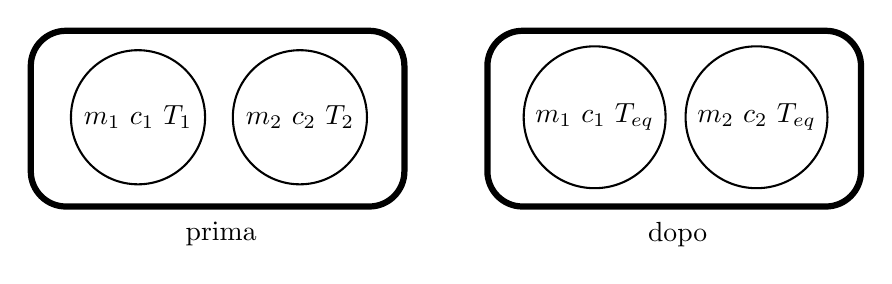
\begin{tikzpicture}[x=0.75pt,y=0.75pt,yscale=-1,xscale=1]
	%uncomment if require: \path (0,300); %set diagram left start at 0, and has height of 300

	%Rounded Rect [id:dp691740350311459] 
	\draw  [line width=2.25]  (61.67,82.6) .. controls (61.67,73.25) and (69.25,65.67) .. (78.6,65.67) -- (224.73,65.67) .. controls (234.09,65.67) and (241.67,73.25) .. (241.67,82.6) -- (241.67,133.4) .. controls (241.67,142.75) and (234.09,150.33) .. (224.73,150.33) -- (78.6,150.33) .. controls (69.25,150.33) and (61.67,142.75) .. (61.67,133.4) -- cycle ;
	%Rounded Rect [id:dp2640122403102567] 
	\draw  [line width=2.25]  (281.67,82.6) .. controls (281.67,73.25) and (289.25,65.67) .. (298.6,65.67) -- (444.73,65.67) .. controls (454.09,65.67) and (461.67,73.25) .. (461.67,82.6) -- (461.67,133.4) .. controls (461.67,142.75) and (454.09,150.33) .. (444.73,150.33) -- (298.6,150.33) .. controls (289.25,150.33) and (281.67,142.75) .. (281.67,133.4) -- cycle ;

	% Text Node
	\draw    (113.33, 107.33) circle [x radius= 32.31, y radius= 32.31]   ;
	\draw (113.33,107.33) node    {$m_{1} \ c_1\ T_{1}$};
	% Text Node
	\draw    (191.33, 107.33) circle [x radius= 32.31, y radius= 32.31]   ;
	\draw (191.33,107.33) node    {$m_{2} \ c_2\ T_{2}$};
	% Text Node
	\draw (153.33,163.67) node   [align=left] {prima};
	% Text Node
	\draw    (333.33, 107.33) circle [x radius= 34.18, y radius= 34.18]   ;
	\draw (333.33,107.33) node    {$m_{1} \ c_1\ T_{eq}$};
	% Text Node
	\draw    (411.33, 107.33) circle [x radius= 34.18, y radius= 34.18]   ;
	\draw (411.33,107.33) node    {$m_{2} \ c_2\ T_{eq}$};
	% Text Node
	\draw (373.33,163.67) node   [align=left] {dopo};

	\end{tikzpicture}
\end{figure}
\FloatBarrier
La temperatura finale sarà la media delle temperature iniziali pesate per la massa del corpo. Si calcola la variazione di entropia per il corpo che si sta scaldando. Bisogna valutare il calore scambiato in maniera reversibile fratto la temperatura, immaginando che il corpo inizialmente alla temperatura $T_1$, si porta fino alla temperatura finale di equilibrio:

\begin{gather*}
	\Delta S_{\text{universo}} = \Delta S_1 + \Delta S_2 \\
	\Delta S_1 = \int_{T_1 }^{T_{eq} } \frac{dQ_{\text{rev} } }{T } = \int_{T_1 }^{T_{eq} } \frac{m_1 c_1 dT}{T} = m_1 c_1\log \frac{T_{eq} }{T_1 } > 0
\end{gather*}

Per il primo corpo si ha un aumento di entropia, per il secondo corpo una diminuzione.

\[
	\Delta S_2 = m_2 c_2 \log \frac{T_2 }{T_{eq} }
\]

Si può dimostrare che la somma fra i due è sempre strettamente positiva.

\paragraph{Esempio 3} Si ha la trasformazione di un un gas perfetto, non ciclica, che lo porta da uno stato $A$ a uno stato $B$. L'espansione è isobara, il gas si trova in un recipiente con pistone mobile. Si valuta cosa accade all'intero universo quando il gas compie una trasformazione prima reversibile e poi irreversibile.

\begin{figure}[htpb]
	\centering

	% Pattern Info
	 
	\tikzset{
	pattern size/.store in=\mcSize, 
	pattern size = 5pt,
	pattern thickness/.store in=\mcThickness, 
	pattern thickness = 0.3pt,
	pattern radius/.store in=\mcRadius, 
	pattern radius = 1pt}
	\makeatletter
	\pgfutil@ifundefined{pgf@pattern@name@_swe55zz85}{
	\pgfdeclarepatternformonly[\mcThickness,\mcSize]{_swe55zz85}
	{\pgfqpoint{0pt}{-\mcThickness}}
	{\pgfpoint{\mcSize}{\mcSize}}
	{\pgfpoint{\mcSize}{\mcSize}}
	{
	\pgfsetcolor{\tikz@pattern@color}
	\pgfsetlinewidth{\mcThickness}
	\pgfpathmoveto{\pgfqpoint{0pt}{\mcSize}}
	\pgfpathlineto{\pgfpoint{\mcSize+\mcThickness}{-\mcThickness}}
	\pgfusepath{stroke}
	}}
	\makeatother

	% Pattern Info
	 
	\tikzset{
	pattern size/.store in=\mcSize, 
	pattern size = 5pt,
	pattern thickness/.store in=\mcThickness, 
	pattern thickness = 0.3pt,
	pattern radius/.store in=\mcRadius, 
	pattern radius = 1pt}
	\makeatletter
	\pgfutil@ifundefined{pgf@pattern@name@_kdvoi9lcg}{
	\pgfdeclarepatternformonly[\mcThickness,\mcSize]{_kdvoi9lcg}
	{\pgfqpoint{0pt}{-\mcThickness}}
	{\pgfpoint{\mcSize}{\mcSize}}
	{\pgfpoint{\mcSize}{\mcSize}}
	{
	\pgfsetcolor{\tikz@pattern@color}
	\pgfsetlinewidth{\mcThickness}
	\pgfpathmoveto{\pgfqpoint{0pt}{\mcSize}}
	\pgfpathlineto{\pgfpoint{\mcSize+\mcThickness}{-\mcThickness}}
	\pgfusepath{stroke}
	}}
	\makeatother
	\tikzset{every picture/.style={line width=0.75pt}} %set default line width to 0.75pt        

	\begin{tikzpicture}[x=0.75pt,y=0.75pt,yscale=-0.9,xscale=0.9]
	%uncomment if require: \path (0,300); %set diagram left start at 0, and has height of 300

	%Shape: Axis 2D [id:dp8058287341299237] 
	\draw  (70,229.2) -- (276.5,229.2)(90.65,84) -- (90.65,245.33) (269.5,224.2) -- (276.5,229.2) -- (269.5,234.2) (85.65,91) -- (90.65,84) -- (95.65,91)  ;
	%Shape: Circle [id:dp9545224062227355] 
	\draw  [fill={rgb, 255:red, 0; green, 0; blue, 0 }  ,fill opacity=1 ] (130.5,151.67) .. controls (130.5,150.47) and (131.47,149.5) .. (132.67,149.5) .. controls (133.86,149.5) and (134.83,150.47) .. (134.83,151.67) .. controls (134.83,152.86) and (133.86,153.83) .. (132.67,153.83) .. controls (131.47,153.83) and (130.5,152.86) .. (130.5,151.67) -- cycle ;
	%Shape: Circle [id:dp47566357433303774] 
	\draw  [fill={rgb, 255:red, 0; green, 0; blue, 0 }  ,fill opacity=1 ] (243.5,151.67) .. controls (243.5,150.47) and (244.47,149.5) .. (245.67,149.5) .. controls (246.86,149.5) and (247.83,150.47) .. (247.83,151.67) .. controls (247.83,152.86) and (246.86,153.83) .. (245.67,153.83) .. controls (244.47,153.83) and (243.5,152.86) .. (243.5,151.67) -- cycle ;
	%Straight Lines [id:da6627242733785048] 
	\draw  [dash pattern={on 4.5pt off 4.5pt}]  (132.67,151.67) -- (245.67,151.67) ;
	%Straight Lines [id:da3245537645654515] 
	\draw    (360,90) -- (360,190) ;
	%Straight Lines [id:da9971336049446691] 
	\draw    (450,90) -- (450,190) ;
	%Straight Lines [id:da7174015175372075] 
	\draw    (360,190) -- (450,190) ;
	%Straight Lines [id:da7830114963304644] 
	\draw [line width=2.25]    (360,131) -- (450,131) ;
	%Shape: Circle [id:dp1526687558537272] 
	\draw  [draw opacity=0][fill={rgb, 255:red, 212; green, 212; blue, 212 }  ,fill opacity=1 ] (388.5,146.13) .. controls (388.5,141.64) and (392.14,138) .. (396.63,138) .. controls (401.11,138) and (404.75,141.64) .. (404.75,146.13) .. controls (404.75,150.61) and (401.11,154.25) .. (396.63,154.25) .. controls (392.14,154.25) and (388.5,150.61) .. (388.5,146.13) -- cycle ;
	%Shape: Circle [id:dp11176800168068657] 
	\draw  [draw opacity=0][fill={rgb, 255:red, 212; green, 212; blue, 212 }  ,fill opacity=1 ] (414,143.13) .. controls (414,138.64) and (417.64,135) .. (422.13,135) .. controls (426.61,135) and (430.25,138.64) .. (430.25,143.13) .. controls (430.25,147.61) and (426.61,151.25) .. (422.13,151.25) .. controls (417.64,151.25) and (414,147.61) .. (414,143.13) -- cycle ;
	%Shape: Circle [id:dp1424335390311502] 
	\draw  [draw opacity=0][fill={rgb, 255:red, 212; green, 212; blue, 212 }  ,fill opacity=1 ] (370.5,157.63) .. controls (370.5,153.14) and (374.14,149.5) .. (378.63,149.5) .. controls (383.11,149.5) and (386.75,153.14) .. (386.75,157.63) .. controls (386.75,162.11) and (383.11,165.75) .. (378.63,165.75) .. controls (374.14,165.75) and (370.5,162.11) .. (370.5,157.63) -- cycle ;
	%Shape: Circle [id:dp6744602416932006] 
	\draw  [draw opacity=0][fill={rgb, 255:red, 212; green, 212; blue, 212 }  ,fill opacity=1 ] (404,160.63) .. controls (404,156.14) and (407.64,152.5) .. (412.13,152.5) .. controls (416.61,152.5) and (420.25,156.14) .. (420.25,160.63) .. controls (420.25,165.11) and (416.61,168.75) .. (412.13,168.75) .. controls (407.64,168.75) and (404,165.11) .. (404,160.63) -- cycle ;
	%Shape: Circle [id:dp5636972303361274] 
	\draw  [draw opacity=0][fill={rgb, 255:red, 212; green, 212; blue, 212 }  ,fill opacity=1 ] (369,177.63) .. controls (369,173.14) and (372.64,169.5) .. (377.13,169.5) .. controls (381.61,169.5) and (385.25,173.14) .. (385.25,177.63) .. controls (385.25,182.11) and (381.61,185.75) .. (377.13,185.75) .. controls (372.64,185.75) and (369,182.11) .. (369,177.63) -- cycle ;
	%Shape: Circle [id:dp7870849322523599] 
	\draw  [draw opacity=0][fill={rgb, 255:red, 212; green, 212; blue, 212 }  ,fill opacity=1 ] (429.5,154.63) .. controls (429.5,150.14) and (433.14,146.5) .. (437.63,146.5) .. controls (442.11,146.5) and (445.75,150.14) .. (445.75,154.63) .. controls (445.75,159.11) and (442.11,162.75) .. (437.63,162.75) .. controls (433.14,162.75) and (429.5,159.11) .. (429.5,154.63) -- cycle ;
	%Shape: Circle [id:dp33718622447106417] 
	\draw  [draw opacity=0][fill={rgb, 255:red, 212; green, 212; blue, 212 }  ,fill opacity=1 ] (389.5,177.63) .. controls (389.5,173.14) and (393.14,169.5) .. (397.63,169.5) .. controls (402.11,169.5) and (405.75,173.14) .. (405.75,177.63) .. controls (405.75,182.11) and (402.11,185.75) .. (397.63,185.75) .. controls (393.14,185.75) and (389.5,182.11) .. (389.5,177.63) -- cycle ;
	%Shape: Circle [id:dp8268977759879512] 
	\draw  [draw opacity=0][fill={rgb, 255:red, 212; green, 212; blue, 212 }  ,fill opacity=1 ] (421,175.13) .. controls (421,170.64) and (424.64,167) .. (429.13,167) .. controls (433.61,167) and (437.25,170.64) .. (437.25,175.13) .. controls (437.25,179.61) and (433.61,183.25) .. (429.13,183.25) .. controls (424.64,183.25) and (421,179.61) .. (421,175.13) -- cycle ;
	%Rounded Rect [id:dp8086986890864896] 
	\draw  [pattern=_swe55zz85,pattern size=6pt,pattern thickness=0.75pt,pattern radius=0pt, pattern color={rgb, 255:red, 155; green, 155; blue, 155}] (350.25,194) .. controls (350.25,191.79) and (352.04,190) .. (354.25,190) -- (456.75,190) .. controls (458.96,190) and (460.75,191.79) .. (460.75,194) -- (460.75,206) .. controls (460.75,208.21) and (458.96,210) .. (456.75,210) -- (354.25,210) .. controls (352.04,210) and (350.25,208.21) .. (350.25,206) -- cycle ;
	%Straight Lines [id:da2900764154820674] 
	\draw    (490,90) -- (490,190) ;
	%Straight Lines [id:da9993641947267269] 
	\draw    (580,90) -- (580,190) ;
	%Straight Lines [id:da3381628855234695] 
	\draw    (490,190) -- (580,190) ;
	%Straight Lines [id:da19064922329872536] 
	\draw [line width=2.25]    (490,97) -- (580,97) ;
	%Shape: Circle [id:dp5535222198453056] 
	\draw  [draw opacity=0][fill={rgb, 255:red, 212; green, 212; blue, 212 }  ,fill opacity=1 ] (496.5,113.46) .. controls (496.5,108.97) and (500.14,105.33) .. (504.63,105.33) .. controls (509.11,105.33) and (512.75,108.97) .. (512.75,113.46) .. controls (512.75,117.95) and (509.11,121.58) .. (504.63,121.58) .. controls (500.14,121.58) and (496.5,117.95) .. (496.5,113.46) -- cycle ;
	%Shape: Circle [id:dp9147284437607994] 
	\draw  [draw opacity=0][fill={rgb, 255:red, 212; green, 212; blue, 212 }  ,fill opacity=1 ] (528.33,114.79) .. controls (528.33,110.3) and (531.97,106.67) .. (536.46,106.67) .. controls (540.95,106.67) and (544.58,110.3) .. (544.58,114.79) .. controls (544.58,119.28) and (540.95,122.92) .. (536.46,122.92) .. controls (531.97,122.92) and (528.33,119.28) .. (528.33,114.79) -- cycle ;
	%Shape: Circle [id:dp9893912797861739] 
	\draw  [draw opacity=0][fill={rgb, 255:red, 212; green, 212; blue, 212 }  ,fill opacity=1 ] (512,130.96) .. controls (512,126.47) and (515.64,122.83) .. (520.13,122.83) .. controls (524.61,122.83) and (528.25,126.47) .. (528.25,130.96) .. controls (528.25,135.45) and (524.61,139.08) .. (520.13,139.08) .. controls (515.64,139.08) and (512,135.45) .. (512,130.96) -- cycle ;
	%Shape: Circle [id:dp8866417359566012] 
	\draw  [draw opacity=0][fill={rgb, 255:red, 212; green, 212; blue, 212 }  ,fill opacity=1 ] (552,125.29) .. controls (552,120.8) and (555.64,117.17) .. (560.13,117.17) .. controls (564.61,117.17) and (568.25,120.8) .. (568.25,125.29) .. controls (568.25,129.78) and (564.61,133.42) .. (560.13,133.42) .. controls (555.64,133.42) and (552,129.78) .. (552,125.29) -- cycle ;
	%Shape: Circle [id:dp4898906214425265] 
	\draw  [draw opacity=0][fill={rgb, 255:red, 212; green, 212; blue, 212 }  ,fill opacity=1 ] (499,177.63) .. controls (499,173.14) and (502.64,169.5) .. (507.13,169.5) .. controls (511.61,169.5) and (515.25,173.14) .. (515.25,177.63) .. controls (515.25,182.11) and (511.61,185.75) .. (507.13,185.75) .. controls (502.64,185.75) and (499,182.11) .. (499,177.63) -- cycle ;
	%Shape: Circle [id:dp4152153683103923] 
	\draw  [draw opacity=0][fill={rgb, 255:red, 212; green, 212; blue, 212 }  ,fill opacity=1 ] (503,152.63) .. controls (503,148.14) and (506.64,144.5) .. (511.13,144.5) .. controls (515.61,144.5) and (519.25,148.14) .. (519.25,152.63) .. controls (519.25,157.11) and (515.61,160.75) .. (511.13,160.75) .. controls (506.64,160.75) and (503,157.11) .. (503,152.63) -- cycle ;
	%Shape: Circle [id:dp32271698384904934] 
	\draw  [draw opacity=0][fill={rgb, 255:red, 212; green, 212; blue, 212 }  ,fill opacity=1 ] (546.83,148.96) .. controls (546.83,144.47) and (550.47,140.83) .. (554.96,140.83) .. controls (559.45,140.83) and (563.08,144.47) .. (563.08,148.96) .. controls (563.08,153.45) and (559.45,157.08) .. (554.96,157.08) .. controls (550.47,157.08) and (546.83,153.45) .. (546.83,148.96) -- cycle ;
	%Shape: Circle [id:dp5475742467603371] 
	\draw  [draw opacity=0][fill={rgb, 255:red, 212; green, 212; blue, 212 }  ,fill opacity=1 ] (551,175.13) .. controls (551,170.64) and (554.64,167) .. (559.13,167) .. controls (563.61,167) and (567.25,170.64) .. (567.25,175.13) .. controls (567.25,179.61) and (563.61,183.25) .. (559.13,183.25) .. controls (554.64,183.25) and (551,179.61) .. (551,175.13) -- cycle ;
	%Rounded Rect [id:dp7271810046379437] 
	\draw  [pattern=_kdvoi9lcg,pattern size=6pt,pattern thickness=0.75pt,pattern radius=0pt, pattern color={rgb, 255:red, 155; green, 155; blue, 155}] (480.25,194) .. controls (480.25,191.79) and (482.04,190) .. (484.25,190) -- (586.75,190) .. controls (588.96,190) and (590.75,191.79) .. (590.75,194) -- (590.75,206) .. controls (590.75,208.21) and (588.96,210) .. (586.75,210) -- (484.25,210) .. controls (482.04,210) and (480.25,208.21) .. (480.25,206) -- cycle ;
	%Straight Lines [id:da829616761495358] 
	\draw    (427.67,225) -- (514,225) ;
	\draw [shift={(517,225)}, rotate = 180] [fill={rgb, 255:red, 0; green, 0; blue, 0 }  ][line width=0.08]  [draw opacity=0] (10.72,-5.15) -- (0,0) -- (10.72,5.15) -- (7.12,0) -- cycle    ;
	%Straight Lines [id:da8315949696634524] 
	\draw    (534,200) .. controls (532.33,198.33) and (532.33,196.67) .. (534,195) .. controls (535.67,193.33) and (535.67,191.67) .. (534,190) .. controls (532.33,188.33) and (532.33,186.67) .. (534,185) .. controls (535.67,183.33) and (535.67,181.67) .. (534,180) .. controls (532.33,178.33) and (532.33,176.67) .. (534,175) .. controls (535.67,173.33) and (535.67,171.67) .. (534,170) -- (534,168.5) -- (534,165.5)(537,200) .. controls (535.33,198.33) and (535.33,196.67) .. (537,195) .. controls (538.67,193.33) and (538.67,191.67) .. (537,190) .. controls (535.33,188.33) and (535.33,186.67) .. (537,185) .. controls (538.67,183.33) and (538.67,181.67) .. (537,180) .. controls (535.33,178.33) and (535.33,176.67) .. (537,175) .. controls (538.67,173.33) and (538.67,171.67) .. (537,170) -- (537,168.5) -- (537,165.5) ;
	\draw [shift={(535.5,156.5)}, rotate = 450] [fill={rgb, 255:red, 0; green, 0; blue, 0 }  ][line width=0.08]  [draw opacity=0] (10.72,-5.15) -- (0,0) -- (10.72,5.15) -- (7.12,0) -- cycle    ;

	% Text Node
	\draw (78,84.33) node    {$p$};
	% Text Node
	\draw (296.67,228.33) node    {$V$};
	% Text Node
	\draw (120.33,162.33) node    {$A$};
	% Text Node
	\draw (256.5,154.83) node    {$B$};
	% Text Node
	\draw (407.33,226.33) node    {$T_{A}$};
	% Text Node
	\draw (537.33,226.33) node    {$T_{B}$};
	% Text Node
	\draw (407.33,111.33) node    {$p_{ext}$};
	% Text Node
	\draw (536.67,78) node    {$p_{ext}$};
	% Text Node
	\draw (345.33,176.33) node    {$T_{A}$};
	% Text Node
	\draw (597.33,176.33) node    {$T_{B}$};

	\end{tikzpicture}
\end{figure}
\FloatBarrier

\textbf{Processo reversibile}. Nell'espandersi il gas si sarà scaldato. Esso avrà bisogno di assorbire calore da un certo serbatoio. La pressione esterna viene mantenuta costante.

\begin{gather*}
	\Delta S_{\text{universo} } = \Delta S_{\text{gas} } + \Delta S_{\text{serb} } \\
	\Delta S_{\text{gas} } = nc_v \log \frac{T_B }{T_A } + nR\log \frac{V_B }{V_A }
\end{gather*}

Se la pressione è costante, volume e temperatura variano linearmente. Quindi:

\[
	pV=nRT \qquad \frac{V_B }{V_A } = \frac{T_B }{T_A } \qquad \Delta S_{\text{gas} } = \log \frac{T_B }{T_A }(c_v+R)n = nc_p\log \frac{T_B }{T_A }
\]

Si fa espandere in maniera molto lenta il gas mettendolo a contatto con infiniti serbatoi, fino a che non si passa dalla temperatura iniziale a quella finale. Bisogna valutare la variazione di entropia di tutti i serbatoi, facendo la somma continua di tutti i calori scambiati da ogni serbatoio. Essi dal punto di vista dei serbatoi sono ceduti quindi ci si aspetta una somma di tanti termini negativi. Il calore scambiato dal gas a pressione costante è:

\[
	\Delta S_{\text{serb} } = \int \frac{dQ_{\text{rev} } }{T} = \int_{T_A }^{T_B } \frac{n c_p dT }{T} = - nc_p\log \frac{T_B }{T_A }
\]

La variazione di entropia dell'universo è uguale a zero perché il processo è reversibile.

\textbf{Processo irreversibile}. Si suppone quindi che il gas venga scaldato alla temperatura $T_B$ mettendolo immediatamente a contatto con il serbatoio $T_B$. Il gas scambierà calore solo con lui. Nel valutare la variazione di entropia del gas, lo stato finale è sempre lo stesso perciò la variazione di entropia dal suo punto di vista sarà la stessa ottenuta per l'esempio precedente. È il serbatoio, che è uno solo, a diminuire l'entropia di una quantità minore di quella vista prima:

\begin{gather*}
	\Delta S_{\text{serb} } = - \frac{Q}{T_B } = \frac{-nc_v(T_B-T_A)}{T_A} \\
	\Delta S_{\text{universo}} = nc_p\log \frac{T_B }{T_A } - nc_p\frac{T_B - T_A  }{T_B } > 0
\end{gather*}

\paragraph{Esempio 4} Si consideri il caso in cui invece il gas segue una trasformazione adiabatica partendo da un certo stato $A$. Si ha un contenitore a pareti isolanti. Il gas in tal caso è isolato termicamente rispetto al resto del mondo. Nel caso di una trasformazione adiabatica il gas è già di suo l'universo termodinamico perché non può scambiare calore con nulla. Si studiano i due casi, reversibile o irreversibile.

\textbf{Processo reversibile}. Non c'è calore scambiato in maniera reversibile. Quindi, quando il gas si espande in maniera adiabatica, l'entropia non può aumentare perché si andrebbe contro il principio di accrescimento dell'entropia. Questo dà un'informazione molto interessante. Se si disegna nel piano di Clapeyron la funzione analitica che descrive la trasformazione reversibile, essa porterà a uno stato $B$ in cui il gas si è espanso, ha diminuito la sua pressione senza scambiare calore. Questa e tutte le curve del tipo $pV^{\gamma}=\text{costante}$ sono curve \textbf{isoentropiche}, dove cioè $S=\text{costante}=S(A)$.

\begin{figure}[htpb]
	\centering

	\tikzset{every picture/.style={line width=0.75pt}} %set default line width to 0.75pt        

	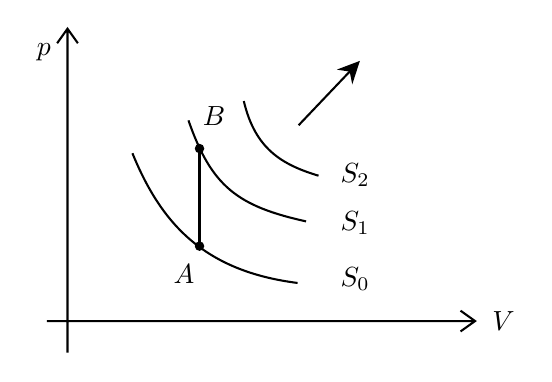
\begin{tikzpicture}[x=0.75pt,y=0.75pt,yscale=-1,xscale=1]
	%uncomment if require: \path (0,300); %set diagram left start at 0, and has height of 300

	%Shape: Axis 2D [id:dp6791519383518894] 
	\draw  (128.5,213.85) -- (334.75,213.85)(138.39,73) -- (138.39,229) (327.75,208.85) -- (334.75,213.85) -- (327.75,218.85) (133.39,80) -- (138.39,73) -- (143.39,80)  ;
	%Straight Lines [id:da040550923790030335] 
	\draw    (277.18,90.67) -- (249.75,119.5) ;
	\draw [shift={(279.25,88.5)}, rotate = 133.58] [fill={rgb, 255:red, 0; green, 0; blue, 0 }  ][line width=0.08]  [draw opacity=0] (10.72,-5.15) -- (0,0) -- (10.72,5.15) -- (7.12,0) -- cycle    ;
	%Curve Lines [id:da05652566709120643] 
	\draw    (169.67,133) .. controls (183.75,167.5) and (204.67,189.83) .. (249.25,195.5) ;
	%Curve Lines [id:da5603647881324592] 
	\draw    (196.67,117.17) .. controls (207.75,149) and (220.25,158.5) .. (253.33,165.83) ;
	%Curve Lines [id:da9493672186610809] 
	\draw    (223.33,107.83) .. controls (228.75,131) and (241.75,138.5) .. (259.33,143.83) ;
	%Straight Lines [id:da8585995024490722] 
	\draw    (202,130) -- (202,178) ;
	%Shape: Circle [id:dp6458738509454554] 
	\draw  [fill={rgb, 255:red, 0; green, 0; blue, 0 }  ,fill opacity=1 ] (200.25,130.75) .. controls (200.25,129.78) and (201.03,129) .. (202,129) .. controls (202.97,129) and (203.75,129.78) .. (203.75,130.75) .. controls (203.75,131.72) and (202.97,132.5) .. (202,132.5) .. controls (201.03,132.5) and (200.25,131.72) .. (200.25,130.75) -- cycle ;
	%Shape: Circle [id:dp08600776298855717] 
	\draw  [fill={rgb, 255:red, 0; green, 0; blue, 0 }  ,fill opacity=1 ] (200.25,177.75) .. controls (200.25,176.78) and (201.03,176) .. (202,176) .. controls (202.97,176) and (203.75,176.78) .. (203.75,177.75) .. controls (203.75,178.72) and (202.97,179.5) .. (202,179.5) .. controls (201.03,179.5) and (200.25,178.72) .. (200.25,177.75) -- cycle ;

	% Text Node
	\draw (127,84.5) node    {$p$};
	% Text Node
	\draw (348.5,214) node    {$V$};
	% Text Node
	\draw (277,193.5) node    {$S_{0}$};
	% Text Node
	\draw (277,166.5) node    {$S_{1}$};
	% Text Node
	\draw (277,143.5) node    {$S_{2}$};
	% Text Node
	\draw (194.5,191) node    {$A$};
	% Text Node
	\draw (209,115) node    {$B$};

	\end{tikzpicture}
\end{figure}
\FloatBarrier
Così come erano state disegnate tutte le isoterme e si era mostrato come la temperatura cresce in una certa direzione, analogamente nel piano di Clapeyron si può disegnare una famiglia di curve isoentropiche del tipo $pV^{\gamma}=\text{costante}$ e l'entropia aumenta nel verso in figura.

\textbf{Processo irreversibile}. Si lascia espandere il gas rimuovendo il peso che c'era sul pistone tutto in una volta. Si arriva in uno stato finale senza scambiare calore. Facendo considerazioni soltanto sulla variazione di entropia del processo, il sistema dovrà arrivare per forza in uno stato diverso, perché altrimenti se passasse per lo stato $B$ pur seguendo un processo irreversibile, si starebbe muovendo lungo una curva isoentropica e quindi arriverebbe ad avere la stessa entropia di $A$, ottenendo una variazione di entropia pari a $0$. Ma se il processo è irreversibile, bisogna aspettarsi che la variazione di entropia del gas sia maggiore di $0$. Si dovrà arrivare in un nuovo stato $B'$ più a sinistra, su una nuova isoentropica con entropia maggiore. Mentre con le isoterme, le isocore e le isobare, partendo da un certo stato si arriva sempre a un altro certo stato, nelle adiabatiche l'irreversiblità porta sempre il gas ad arrivare ad uno stato finale diverso.

Si osservi inoltre che quando si passa tramite un'adiabatica irreversibile da uno stato $A$ ad uno stato $B$, con $S_B$ necessariamente maggiore di $S_A$, non è più possibile ritornare in $A$ adiabaticamente, né in modo reversibile né irreversibile, perché in ogni caso ciò comporterebbe $\Delta S<0$. Si può allora dire che una trasformazione adiabatica irreversibile presenta una \emph{irreversibilità in senso stretto}. Questo non è il caso di altre trasformazioni irreversibili, perché in generale l'intervento dell'ambiente con le sue variazioni di entropia rende possibile il ritorno allo stato iniziale con lo stesso tipo di trasformazione senza violare il principio di aumento dell'entropia dell'universo termodinamico.
In altre parole, due stati collegati con un'adiabatica irreversibile hanno necessariamente entropia diversa e non possono quindi essere collegati anche con un'adiabatica reversibile, che è un'isoentropica.

La famiglia delle curve adiabatiche reversibili sono caratterizzate dalla relazione:

\[
	pV^{\gamma } = \text{costante}
\]

Tale famiglia è rappresentata in figura. Se ci si muove su una di queste curve, ci si sta muovendo su una trasformazione a entropia costante.

Come si fa a capire se spostandosi dalla curva a entropia $S_0$ a quella a entropia $S_1$ aumenta $S$?
Si supponga di prendere uno stato qualunque $A$ sulla curva $S_0$ e di muoversi con un' isocora su uno stato $B$ che è ad un certo punto della curva $S_1$ facendo fondamentalmente un riscaldamento a volume costante. Si scrive la variazione di entropia da stato $A$ a stato $B$ per la variazione di entropia di un gas perfetto.

\[
	\Delta S = S(B)-S(A) = nc_v\log \frac{T_2 }{T_1 } + nR \log \frac{V_2 }{V_1 }
\]

Nel caso che si sta considerando il secondo addendo non c'è, rimane solo il primo. $T_B$ è maggiore di $T_A$ perché ci si sposta su un'isoterma più a destra. È quindi un riscaldamento e $S(B)>S(A)$. Se si vanno a disegnare le varie isoentropiche nel piano di Clapeyron, si vede fondamentalmente che l'entropia cresce nel verso della freccia.
Mettendo le famiglie di curve, isoterme e isoentropiche, si possono fare delle considerazioni interessanti sulle porzioni del piano di Clapeyron che non sono permesse. Si sfrutta il principio di accrescimento dell'entropia dell'universo. Ci si pone in uno stato $A$ e in tale stato si vanno a disegnare la curva isoterma e quella isoentropica che passano per quello stato.

\begin{figure}[htpb]
	\centering

	\tikzset{every picture/.style={line width=0.75pt}} %set default line width to 0.75pt        

	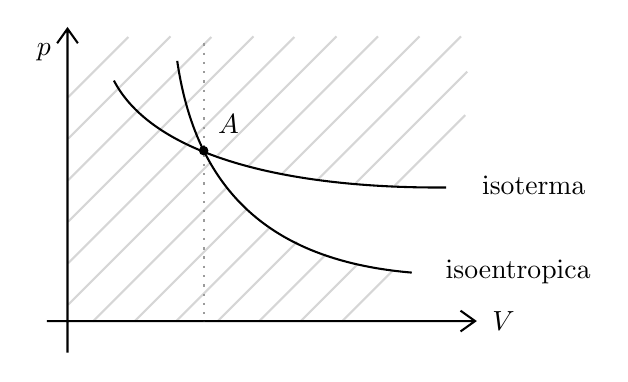
\begin{tikzpicture}[x=0.75pt,y=0.75pt,yscale=-1,xscale=1]
	%uncomment if require: \path (0,300); %set diagram left start at 0, and has height of 300

	%Straight Lines [id:da0741049687567581] 
	\draw [color={rgb, 255:red, 214; green, 214; blue, 214 }  ,draw opacity=1 ]   (295,250.67) -- (270.67,275) ;
	%Straight Lines [id:da012561168898262531] 
	\draw [color={rgb, 255:red, 214; green, 214; blue, 214 }  ,draw opacity=1 ]   (167.67,138) -- (138.67,167) ;
	%Straight Lines [id:da6370578645029346] 
	\draw [color={rgb, 255:red, 214; green, 214; blue, 214 }  ,draw opacity=1 ]   (188,137.67) -- (138.67,187) ;
	%Straight Lines [id:da11423227056922736] 
	\draw [color={rgb, 255:red, 214; green, 214; blue, 214 }  ,draw opacity=1 ]   (207.67,138) -- (138.67,207) ;
	%Straight Lines [id:da808109097546619] 
	\draw [color={rgb, 255:red, 214; green, 214; blue, 214 }  ,draw opacity=1 ]   (228,137.67) -- (138.67,227) ;
	%Straight Lines [id:da5056432870620773] 
	\draw [color={rgb, 255:red, 214; green, 214; blue, 214 }  ,draw opacity=1 ]   (247.67,138) -- (138.67,247) ;
	%Straight Lines [id:da9799464593161868] 
	\draw [color={rgb, 255:red, 214; green, 214; blue, 214 }  ,draw opacity=1 ]   (207,198.67) -- (138.67,267) ;
	%Straight Lines [id:da7504849115865206] 
	\draw [color={rgb, 255:red, 214; green, 214; blue, 214 }  ,draw opacity=1 ]   (215,210.67) -- (150.67,275) ;
	%Straight Lines [id:da7433407923845881] 
	\draw [color={rgb, 255:red, 214; green, 214; blue, 214 }  ,draw opacity=1 ]   (225,220.67) -- (170.67,275) ;
	%Straight Lines [id:da38984121270333993] 
	\draw [color={rgb, 255:red, 214; green, 214; blue, 214 }  ,draw opacity=1 ]   (236,229.67) -- (190.67,275) ;
	%Straight Lines [id:da654830155031356] 
	\draw [color={rgb, 255:red, 214; green, 214; blue, 214 }  ,draw opacity=1 ]   (249,236.67) -- (210.67,275) ;
	%Straight Lines [id:da6109502725467904] 
	\draw [color={rgb, 255:red, 214; green, 214; blue, 214 }  ,draw opacity=1 ]   (263,242.67) -- (230.67,275) ;
	%Straight Lines [id:da73216921122118] 
	\draw [color={rgb, 255:red, 214; green, 214; blue, 214 }  ,draw opacity=1 ]   (278,247.67) -- (250.67,275) ;
	%Straight Lines [id:da23448718854163642] 
	\draw [color={rgb, 255:red, 214; green, 214; blue, 214 }  ,draw opacity=1 ]   (288,137.67) -- (225.67,200) ;
	%Straight Lines [id:da7315296214909419] 
	\draw [color={rgb, 255:red, 214; green, 214; blue, 214 }  ,draw opacity=1 ]   (308,137.67) -- (241.67,204) ;
	%Straight Lines [id:da34186492151441694] 
	\draw [color={rgb, 255:red, 214; green, 214; blue, 214 }  ,draw opacity=1 ]   (328,137.67) -- (258.67,207) ;
	%Straight Lines [id:da4290520340827755] 
	\draw [color={rgb, 255:red, 214; green, 214; blue, 214 }  ,draw opacity=1 ]   (331,154.67) -- (276.67,209) ;
	%Straight Lines [id:da5480858567328142] 
	\draw [color={rgb, 255:red, 214; green, 214; blue, 214 }  ,draw opacity=1 ]   (330,175.67) -- (295.67,210) ;
	%Shape: Axis 2D [id:dp9314597919243865] 
	\draw  (128.5,274.85) -- (334.75,274.85)(138.39,134) -- (138.39,290) (327.75,269.85) -- (334.75,274.85) -- (327.75,279.85) (133.39,141) -- (138.39,134) -- (143.39,141)  ;
	%Curve Lines [id:da49963022668914747] 
	\draw    (160.75,159) .. controls (179.25,194.5) and (241.75,211) .. (320.75,210.5) ;
	%Curve Lines [id:da2838240681359938] 
	\draw    (191.25,149.5) .. controls (200.75,215) and (239.25,246) .. (304.25,251.5) ;
	%Straight Lines [id:da9931014522236101] 
	\draw [color={rgb, 255:red, 155; green, 155; blue, 155 }  ,draw opacity=1 ] [dash pattern={on 0.84pt off 2.51pt}]  (204,141) -- (204,275) ;
	%Shape: Circle [id:dp8807672671591289] 
	\draw  [fill={rgb, 255:red, 0; green, 0; blue, 0 }  ,fill opacity=1 ] (202.25,192.75) .. controls (202.25,191.78) and (203.03,191) .. (204,191) .. controls (204.97,191) and (205.75,191.78) .. (205.75,192.75) .. controls (205.75,193.72) and (204.97,194.5) .. (204,194.5) .. controls (203.03,194.5) and (202.25,193.72) .. (202.25,192.75) -- cycle ;
	%Straight Lines [id:da5075107359701121] 
	\draw [color={rgb, 255:red, 214; green, 214; blue, 214 }  ,draw opacity=1 ]   (268,137.67) -- (210.67,195) ;

	% Text Node
	\draw (127,145.5) node    {$p$};
	% Text Node
	\draw (348.5,275) node    {$V$};
	% Text Node
	\draw (216,180) node    {$A$};
	% Text Node
	\draw (355.5,251) node   [align=left] {isoentropica};
	% Text Node
	\draw (363,209.5) node   [align=left] {isoterma};

	\end{tikzpicture}
\end{figure}
\FloatBarrier

\section{Porzioni di piano permesse dal II principio}

Si vuol far espandere il gas con una trasformazione reale, quindi irreversibile, adiabatica, che porta da $A$ ad uno stato $B'$. Qual è sia là porzione di piano in cui può trovarsi $B'$?
È intanto permessa quella porzione di piano per cui $V>V_A$. Essendo adiabatica, la variazione di entropia del gas è uguale alla variazione di entropia dell'universo. Poiché è irreversibile la variazione di entropia del gas deve essere sicuramente positiva. Sono permesse solo le porzioni di spazio al di sopra della isoentropica passante per $A$.
Quando si fa espandere un gas si può fare una considerazione sulla temperatura. Infatti se lo si fa espandere non permettendogli di assorbire calore dall'ambiente costante, esso si raffredda. Quindi può stare solo in quella regione di piano al di sotto della isoterma passante per $A$.
Questo discorso fa capire che, mentre con il primo principio della termodinamica considerando questa situazione si sarebbero poste delle limitazioni solo riguardo al fatto che il volume deve aumentare e la temperatura diminuire, si capisce che ci sono regioni di spazio non permesse a causa del fatto che l'entropia dell'universo deve sempre aumentare. Il secondo principio della termodinamica pone dei limiti al modo in cui il sistema deve evolvere, alle possibili trasformazioni che si possono realizzare nella pratica. Ci si rende conto che la situazione $\mathcal{L} = -\Delta U$ è molto particolare, nel senso che la maggior parte delle trasformazioni di un sistema termodinamico avvengono solo se c'è scambio di calore.

\section{Il piano di Gibbs}

Esiste un altro piano interessante noto come \textbf{piano di Gibbs}. In esso si va a disegnare lo stato di un sistema termodinamico in funzione delle variabili termodinamiche temperatura e entropia. L'entropia infatti, essendo funzione di stato, può essere scelta come variabile indipendente per descrivere, insieme ad una seconda variabile indipendente opportunamente scelta, lo stato termodinamico di un sistema. Nel piano di Clapeyron, se si prende il prodotto fra la variabile pressione e un infinitesimo della variabile sulle $x$, il volume, si ottiene un'energia, in particolare il lavoro compiuto da un sistema termodinamico.
Si riprenda allora la variazione di entropia finita fra due stati. Essa è uguale all'integrale del calore infinitesimo scambiato in maniera reversibile su $T$ integrato fra stato iniziale e finale. Questa relazione, scritta in termini finiti, si potrebbe anche esprimere come quantità infinitesima fra due stati molto vicini.

\[
	dS = \frac{dQ_{\text{rev} } }{T} \implies T\,dS = dQ_{\text{rev} }
\]

Così come si può rappresentare una trasformazione reversibile nel piano $pV$,  e valutarne l'area sottesa, che rappresenta il lavoro reversibile fatto dal gas, in maniera del tutto analoga, se si disegna nel piano $TS$ una qualunque trasformazione reversibile, l'area sottesa dalla curva è il calore scambiato durante la trasformazione in maniera reversibile. È interessante notare come si disegna il ciclo di Carnot nel piano di Gibbs.

\begin{figure}[htpb]
	\centering

	\tikzset{every picture/.style={line width=0.75pt}} %set default line width to 0.75pt        

	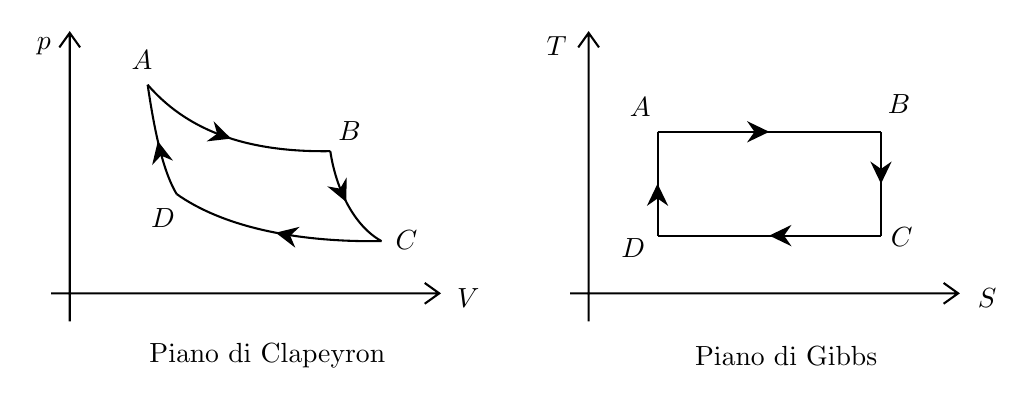
\begin{tikzpicture}[x=0.75pt,y=0.75pt,yscale=-1,xscale=1]
	%uncomment if require: \path (0,300); %set diagram left start at 0, and has height of 300

	%Shape: Axis 2D [id:dp6207852838282175] 
	\draw  (68.5,188.5) -- (255.5,188.5)(77.46,63) -- (77.46,202) (248.5,183.5) -- (255.5,188.5) -- (248.5,193.5) (72.46,70) -- (77.46,63) -- (82.46,70)  ;
	%Curve Lines [id:da17880604881557938] 
	\draw    (115,88) .. controls (132.33,108) and (159,120.67) .. (203,120) ;
	\draw [shift={(155.22,113.94)}, rotate = 199.15] [fill={rgb, 255:red, 0; green, 0; blue, 0 }  ][line width=0.08]  [draw opacity=0] (10.72,-5.15) -- (0,0) -- (10.72,5.15) -- (7.12,0) -- cycle    ;
	%Curve Lines [id:da7787902897460273] 
	\draw    (203,120) .. controls (205.67,138) and (214.33,156) .. (227.67,163.33) ;
	\draw [shift={(210.72,144.51)}, rotate = 245.12] [fill={rgb, 255:red, 0; green, 0; blue, 0 }  ][line width=0.08]  [draw opacity=0] (10.72,-5.15) -- (0,0) -- (10.72,5.15) -- (7.12,0) -- cycle    ;
	%Curve Lines [id:da5376663670104085] 
	\draw    (115,88) .. controls (117.67,106) and (121.67,128.67) .. (129,140.67) ;
	\draw [shift={(119.92,115.17)}, rotate = 77.79] [fill={rgb, 255:red, 0; green, 0; blue, 0 }  ][line width=0.08]  [draw opacity=0] (10.72,-5.15) -- (0,0) -- (10.72,5.15) -- (7.12,0) -- cycle    ;
	%Curve Lines [id:da706592795484827] 
	\draw    (129,140.67) .. controls (149.67,155.33) and (183.67,164) .. (227.67,163.33) ;
	\draw [shift={(176.72,159.28)}, rotate = 11.86] [fill={rgb, 255:red, 0; green, 0; blue, 0 }  ][line width=0.08]  [draw opacity=0] (10.72,-5.15) -- (0,0) -- (10.72,5.15) -- (7.12,0) -- cycle    ;
	%Shape: Axis 2D [id:dp4893064797014206] 
	\draw  (318.5,188.5) -- (505.5,188.5)(327.46,63) -- (327.46,202) (498.5,183.5) -- (505.5,188.5) -- (498.5,193.5) (322.46,70) -- (327.46,63) -- (332.46,70)  ;
	%Straight Lines [id:da6745812171453553] 
	\draw    (360.67,110.67) -- (468.33,110.67) ;
	%Straight Lines [id:da09160897438719262] 
	\draw    (360.67,110.67) -- (468.33,110.67) ;
	\draw [shift={(414.5,110.67)}, rotate = 180] [fill={rgb, 255:red, 0; green, 0; blue, 0 }  ][line width=0.08]  [draw opacity=0] (10.72,-5.15) -- (0,0) -- (10.72,5.15) -- (7.12,0) -- cycle    ;
	%Straight Lines [id:da3351262724181472] 
	\draw    (360.67,160.67) -- (468.33,160.67) ;
	\draw [shift={(414.5,160.67)}, rotate = 0] [fill={rgb, 255:red, 0; green, 0; blue, 0 }  ][line width=0.08]  [draw opacity=0] (10.72,-5.15) -- (0,0) -- (10.72,5.15) -- (7.12,0) -- cycle    ;
	%Straight Lines [id:da7493185984968482] 
	\draw    (468.33,160.67) -- (468.33,110.67) ;
	\draw [shift={(468.33,135.67)}, rotate = 270] [fill={rgb, 255:red, 0; green, 0; blue, 0 }  ][line width=0.08]  [draw opacity=0] (10.72,-5.15) -- (0,0) -- (10.72,5.15) -- (7.12,0) -- cycle    ;
	%Straight Lines [id:da37877542289534505] 
	\draw    (360.67,160.67) -- (360.67,110.67) ;
	\draw [shift={(360.67,135.67)}, rotate = 450] [fill={rgb, 255:red, 0; green, 0; blue, 0 }  ][line width=0.08]  [draw opacity=0] (10.72,-5.15) -- (0,0) -- (10.72,5.15) -- (7.12,0) -- cycle    ;

	% Text Node
	\draw (65,69.5) node    {$p$};
	% Text Node
	\draw (269.5,191) node    {$V$};
	% Text Node
	\draw (312,69.5) node    {$T$};
	% Text Node
	\draw (519.5,191) node    {$S$};
	% Text Node
	\draw (352.33,98.83) node    {$A$};
	% Text Node
	\draw (477,97.5) node    {$B$};
	% Text Node
	\draw (478.33,161.5) node    {$C$};
	% Text Node
	\draw (349,166.83) node    {$D$};
	% Text Node
	\draw (112.33,76.17) node    {$A$};
	% Text Node
	\draw (212.33,110.17) node    {$B$};
	% Text Node
	\draw (239.67,162.83) node    {$C$};
	% Text Node
	\draw (122.33,152.17) node    {$D$};
	% Text Node
	\draw (172.67,218.67) node   [align=left] {Piano di Clapeyron};
	% Text Node
	\draw (422.67,218.67) node   [align=left] {Piano di Gibbs};

	\end{tikzpicture}
\end{figure}
\FloatBarrier
Le isoterme si diagrammano come rette orizzontali alle quote rispettivamente $T_1$ e $T_2$. Le isoentropiche invece si rappresentano come rette verticali. Il piano di Gibbs è comodo perché si può calcolare direttamente dal grafico il rendimento di una macchina reversibile. Esso è dato dal rapporto tra l'area racchiusa dal ciclo (che rappresenta il lavoro per il primo principio della termodinamica, oltre che al calore) e quella sottesa dalla curva superiore.
Risulta così evidente che il rendimento della macchina è inferiore all'unità.

Si consideri ad esempio una macchina più complicata di Carnot che scambia calore con tre serbatoi. Il ciclo è rappresentato in figura su entrambi i piani.

\begin{figure}[htpb]
	\centering

	% Pattern Info
	 
	\tikzset{
	pattern size/.store in=\mcSize, 
	pattern size = 5pt,
	pattern thickness/.store in=\mcThickness, 
	pattern thickness = 0.3pt,
	pattern radius/.store in=\mcRadius, 
	pattern radius = 1pt}
	\makeatletter
	\pgfutil@ifundefined{pgf@pattern@name@_25zm4e1hf lines}{
	\pgfdeclarepatternformonly[\mcThickness,\mcSize]{_25zm4e1hf}
	{\pgfqpoint{0pt}{0pt}}
	{\pgfpoint{\mcSize+\mcThickness}{\mcSize+\mcThickness}}
	{\pgfpoint{\mcSize}{\mcSize}}
	{\pgfsetcolor{\tikz@pattern@color}
	\pgfsetlinewidth{\mcThickness}
	\pgfpathmoveto{\pgfpointorigin}
	\pgfpathlineto{\pgfpoint{\mcSize}{0}}
	\pgfusepath{stroke}}}
	\makeatother

	% Pattern Info
	 
	\tikzset{
	pattern size/.store in=\mcSize, 
	pattern size = 5pt,
	pattern thickness/.store in=\mcThickness, 
	pattern thickness = 0.3pt,
	pattern radius/.store in=\mcRadius, 
	pattern radius = 1pt}
	\makeatletter
	\pgfutil@ifundefined{pgf@pattern@name@_063m0qo2e}{
	\makeatletter
	\pgfdeclarepatternformonly[\mcRadius,\mcThickness,\mcSize]{_063m0qo2e}
	{\pgfpoint{-0.5*\mcSize}{-0.5*\mcSize}}
	{\pgfpoint{0.5*\mcSize}{0.5*\mcSize}}
	{\pgfpoint{\mcSize}{\mcSize}}
	{
	\pgfsetcolor{\tikz@pattern@color}
	\pgfsetlinewidth{\mcThickness}
	\pgfpathcircle\pgfpointorigin{\mcRadius}
	\pgfusepath{stroke}
	}}
	\makeatother

	% Pattern Info
	 
	\tikzset{
	pattern size/.store in=\mcSize, 
	pattern size = 5pt,
	pattern thickness/.store in=\mcThickness, 
	pattern thickness = 0.3pt,
	pattern radius/.store in=\mcRadius, 
	pattern radius = 1pt}
	\makeatletter
	\pgfutil@ifundefined{pgf@pattern@name@_u93ic1mtb}{
	\pgfdeclarepatternformonly[\mcThickness,\mcSize]{_u93ic1mtb}
	{\pgfqpoint{0pt}{0pt}}
	{\pgfpoint{\mcSize+\mcThickness}{\mcSize+\mcThickness}}
	{\pgfpoint{\mcSize}{\mcSize}}
	{
	\pgfsetcolor{\tikz@pattern@color}
	\pgfsetlinewidth{\mcThickness}
	\pgfpathmoveto{\pgfqpoint{0pt}{0pt}}
	\pgfpathlineto{\pgfpoint{\mcSize+\mcThickness}{\mcSize+\mcThickness}}
	\pgfusepath{stroke}
	}}
	\makeatother
	\tikzset{every picture/.style={line width=0.75pt}} %set default line width to 0.75pt        

	\begin{tikzpicture}[x=0.75pt,y=0.75pt,yscale=-1,xscale=1]
	%uncomment if require: \path (0,300); %set diagram left start at 0, and has height of 300

	%Shape: Rectangle [id:dp35068313855016964] 
	\draw  [draw opacity=0][pattern=_25zm4e1hf,pattern size=2.25pt,pattern thickness=0.75pt,pattern radius=0pt, pattern color={rgb, 255:red, 155; green, 155; blue, 155}] (360.67,160.67) -- (468.33,160.67) -- (468.33,186.8) -- (360.67,186.8) -- cycle ;
	%Shape: Rectangle [id:dp47426860666934667] 
	\draw  [draw opacity=0][pattern=_063m0qo2e,pattern size=6pt,pattern thickness=0.75pt,pattern radius=0.75pt, pattern color={rgb, 255:red, 155; green, 155; blue, 155}] (418.33,110.67) -- (468.33,110.67) -- (468.33,187.2) -- (418.33,187.2) -- cycle ;
	%Shape: Rectangle [id:dp593521786657115] 
	\draw  [draw opacity=0][pattern=_u93ic1mtb,pattern size=6pt,pattern thickness=0.75pt,pattern radius=0pt, pattern color={rgb, 255:red, 155; green, 155; blue, 155}] (360.67,60.67) -- (418.33,60.67) -- (418.33,186.8) -- (360.67,186.8) -- cycle ;
	%Shape: Axis 2D [id:dp42718451569737725] 
	\draw  (68.5,186.98) -- (260.67,186.98)(77.71,47.33) -- (77.71,202) (253.67,181.98) -- (260.67,186.98) -- (253.67,191.98) (72.71,54.33) -- (77.71,47.33) -- (82.71,54.33)  ;
	%Curve Lines [id:da6495179254879908] 
	\draw    (101.67,56.33) .. controls (123.33,69) and (130,76.33) .. (162,76.33) ;
	\draw [shift={(130.25,71.97)}, rotate = 202.63] [fill={rgb, 255:red, 0; green, 0; blue, 0 }  ][line width=0.08]  [draw opacity=0] (10.72,-5.15) -- (0,0) -- (10.72,5.15) -- (7.12,0) -- cycle    ;
	%Curve Lines [id:da8141226896387221] 
	\draw    (162,76.33) .. controls (164.67,94.33) and (171.33,109) .. (180.67,121) ;
	\draw [shift={(168.46,100.02)}, rotate = 249.3] [fill={rgb, 255:red, 0; green, 0; blue, 0 }  ][line width=0.08]  [draw opacity=0] (10.72,-5.15) -- (0,0) -- (10.72,5.15) -- (7.12,0) -- cycle    ;
	%Curve Lines [id:da13989607523506598] 
	\draw    (101.67,56.33) .. controls (104.33,74.33) and (110.67,125.33) .. (127.33,153.33) ;
	\draw [shift={(110.37,106.1)}, rotate = 77.43] [fill={rgb, 255:red, 0; green, 0; blue, 0 }  ][line width=0.08]  [draw opacity=0] (10.72,-5.15) -- (0,0) -- (10.72,5.15) -- (7.12,0) -- cycle    ;
	%Curve Lines [id:da5225465849499047] 
	\draw    (127.33,153.33) .. controls (144.67,164.67) and (191.33,173) .. (235.33,172.33) ;
	\draw [shift={(180.24,168.77)}, rotate = 8.85] [fill={rgb, 255:red, 0; green, 0; blue, 0 }  ][line width=0.08]  [draw opacity=0] (10.72,-5.15) -- (0,0) -- (10.72,5.15) -- (7.12,0) -- cycle    ;
	%Shape: Axis 2D [id:dp025738552451401775] 
	\draw  (318.5,187.3) -- (505.5,187.3)(327.46,50.67) -- (327.46,202) (498.5,182.3) -- (505.5,187.3) -- (498.5,192.3) (322.46,57.67) -- (327.46,50.67) -- (332.46,57.67)  ;
	%Straight Lines [id:da17184396492467124] 
	\draw    (360.67,60.67) -- (418.33,60.67) ;
	\draw [shift={(389.5,60.67)}, rotate = 180] [fill={rgb, 255:red, 0; green, 0; blue, 0 }  ][line width=0.08]  [draw opacity=0] (10.72,-5.15) -- (0,0) -- (10.72,5.15) -- (7.12,0) -- cycle    ;
	%Straight Lines [id:da3328308427577038] 
	\draw    (418.33,110.67) -- (468.33,110.67) ;
	\draw [shift={(443.33,110.67)}, rotate = 180] [fill={rgb, 255:red, 0; green, 0; blue, 0 }  ][line width=0.08]  [draw opacity=0] (10.72,-5.15) -- (0,0) -- (10.72,5.15) -- (7.12,0) -- cycle    ;
	%Straight Lines [id:da9505803052171997] 
	\draw    (360.67,160.67) -- (468.33,160.67) ;
	\draw [shift={(414.5,160.67)}, rotate = 0] [fill={rgb, 255:red, 0; green, 0; blue, 0 }  ][line width=0.08]  [draw opacity=0] (10.72,-5.15) -- (0,0) -- (10.72,5.15) -- (7.12,0) -- cycle    ;
	%Straight Lines [id:da5801133154586786] 
	\draw    (468.33,160.67) -- (468.33,110.67) ;
	\draw [shift={(468.33,135.67)}, rotate = 270] [fill={rgb, 255:red, 0; green, 0; blue, 0 }  ][line width=0.08]  [draw opacity=0] (10.72,-5.15) -- (0,0) -- (10.72,5.15) -- (7.12,0) -- cycle    ;
	%Straight Lines [id:da6975245276911515] 
	\draw    (360.67,160.67) -- (360.67,60.67) ;
	\draw [shift={(360.67,110.67)}, rotate = 450] [fill={rgb, 255:red, 0; green, 0; blue, 0 }  ][line width=0.08]  [draw opacity=0] (10.72,-5.15) -- (0,0) -- (10.72,5.15) -- (7.12,0) -- cycle    ;
	%Curve Lines [id:da6975020862261498] 
	\draw    (180.67,121) .. controls (196,129) and (202.67,131.67) .. (221.33,131.67) ;
	\draw [shift={(200.28,129.48)}, rotate = 198.23] [fill={rgb, 255:red, 0; green, 0; blue, 0 }  ][line width=0.08]  [draw opacity=0] (10.72,-5.15) -- (0,0) -- (10.72,5.15) -- (7.12,0) -- cycle    ;
	%Curve Lines [id:da8289401327108623] 
	\draw    (221.33,131.67) .. controls (224,149.67) and (226,160.33) .. (235.33,172.33) ;
	\draw [shift={(225.48,153.09)}, rotate = 255.79000000000002] [fill={rgb, 255:red, 0; green, 0; blue, 0 }  ][line width=0.08]  [draw opacity=0] (10.72,-5.15) -- (0,0) -- (10.72,5.15) -- (7.12,0) -- cycle    ;
	%Straight Lines [id:da3869861390769662] 
	\draw    (418.33,110.67) -- (418.33,60.67) ;
	\draw [shift={(418.33,85.67)}, rotate = 270] [fill={rgb, 255:red, 0; green, 0; blue, 0 }  ][line width=0.08]  [draw opacity=0] (10.72,-5.15) -- (0,0) -- (10.72,5.15) -- (7.12,0) -- cycle    ;
	%Straight Lines [id:da5224236485541403] 
	\draw    (139.17,50.67) .. controls (140.84,52.34) and (140.84,54) .. (139.17,55.67) .. controls (137.5,57.34) and (137.5,59) .. (139.17,60.67) .. controls (140.84,62.34) and (140.84,64) .. (139.17,65.67) .. controls (137.5,67.34) and (137.5,69) .. (139.17,70.67) .. controls (140.84,72.34) and (140.84,74) .. (139.17,75.67) .. controls (137.5,77.34) and (137.5,79) .. (139.17,80.67) -- (139.17,83) -- (139.17,86)(136.17,50.67) .. controls (137.84,52.34) and (137.84,54) .. (136.17,55.67) .. controls (134.5,57.34) and (134.5,59) .. (136.17,60.67) .. controls (137.84,62.34) and (137.84,64) .. (136.17,65.67) .. controls (134.5,67.34) and (134.5,69) .. (136.17,70.67) .. controls (137.84,72.34) and (137.84,74) .. (136.17,75.67) .. controls (134.5,77.34) and (134.5,79) .. (136.17,80.67) -- (136.17,83) -- (136.17,86) ;
	\draw [shift={(137.67,94)}, rotate = 270] [color={rgb, 255:red, 0; green, 0; blue, 0 }  ][line width=0.75]    (10.93,-3.29) .. controls (6.95,-1.4) and (3.31,-0.3) .. (0,0) .. controls (3.31,0.3) and (6.95,1.4) .. (10.93,3.29)   ;
	%Straight Lines [id:da491624189292325] 
	\draw    (207.17,106) .. controls (208.84,107.67) and (208.84,109.33) .. (207.17,111) .. controls (205.5,112.67) and (205.5,114.33) .. (207.17,116) .. controls (208.84,117.67) and (208.84,119.33) .. (207.17,121) .. controls (205.5,122.67) and (205.5,124.33) .. (207.17,126) .. controls (208.84,127.67) and (208.84,129.33) .. (207.17,131) .. controls (205.5,132.67) and (205.5,134.33) .. (207.17,136) -- (207.17,138.33) -- (207.17,141.33)(204.17,106) .. controls (205.84,107.67) and (205.84,109.33) .. (204.17,111) .. controls (202.5,112.67) and (202.5,114.33) .. (204.17,116) .. controls (205.84,117.67) and (205.84,119.33) .. (204.17,121) .. controls (202.5,122.67) and (202.5,124.33) .. (204.17,126) .. controls (205.84,127.67) and (205.84,129.33) .. (204.17,131) .. controls (202.5,132.67) and (202.5,134.33) .. (204.17,136) -- (204.17,138.33) -- (204.17,141.33) ;
	\draw [shift={(205.67,149.33)}, rotate = 270] [color={rgb, 255:red, 0; green, 0; blue, 0 }  ][line width=0.75]    (10.93,-3.29) .. controls (6.95,-1.4) and (3.31,-0.3) .. (0,0) .. controls (3.31,0.3) and (6.95,1.4) .. (10.93,3.29)   ;
	%Straight Lines [id:da8687331853501177] 
	\draw    (161.17,145.33) .. controls (162.84,147) and (162.84,148.66) .. (161.17,150.33) .. controls (159.5,152) and (159.5,153.66) .. (161.17,155.33) .. controls (162.84,157) and (162.84,158.66) .. (161.17,160.33) .. controls (159.5,162) and (159.5,163.66) .. (161.17,165.33) .. controls (162.84,167) and (162.84,168.66) .. (161.17,170.33) -- (161.17,171.67) -- (161.17,174.67)(158.17,145.33) .. controls (159.84,147) and (159.84,148.66) .. (158.17,150.33) .. controls (156.5,152) and (156.5,153.66) .. (158.17,155.33) .. controls (159.84,157) and (159.84,158.66) .. (158.17,160.33) .. controls (156.5,162) and (156.5,163.66) .. (158.17,165.33) .. controls (159.84,167) and (159.84,168.66) .. (158.17,170.33) -- (158.17,171.67) -- (158.17,174.67) ;
	\draw [shift={(159.67,182.67)}, rotate = 270] [color={rgb, 255:red, 0; green, 0; blue, 0 }  ][line width=0.75]    (10.93,-3.29) .. controls (6.95,-1.4) and (3.31,-0.3) .. (0,0) .. controls (3.31,0.3) and (6.95,1.4) .. (10.93,3.29)   ;
	%Straight Lines [id:da9329491022140817] 
	\draw    (397.17,43) .. controls (398.84,44.67) and (398.84,46.33) .. (397.17,48) .. controls (395.5,49.67) and (395.5,51.33) .. (397.17,53) .. controls (398.84,54.67) and (398.84,56.33) .. (397.17,58) .. controls (395.5,59.67) and (395.5,61.33) .. (397.17,63) .. controls (398.84,64.67) and (398.84,66.33) .. (397.17,68) -- (397.17,69.67) -- (397.17,72.67)(394.17,43) .. controls (395.84,44.67) and (395.84,46.33) .. (394.17,48) .. controls (392.5,49.67) and (392.5,51.33) .. (394.17,53) .. controls (395.84,54.67) and (395.84,56.33) .. (394.17,58) .. controls (392.5,59.67) and (392.5,61.33) .. (394.17,63) .. controls (395.84,64.67) and (395.84,66.33) .. (394.17,68) -- (394.17,69.67) -- (394.17,72.67) ;
	\draw [shift={(395.67,80.67)}, rotate = 270] [color={rgb, 255:red, 0; green, 0; blue, 0 }  ][line width=0.75]    (10.93,-3.29) .. controls (6.95,-1.4) and (3.31,-0.3) .. (0,0) .. controls (3.31,0.3) and (6.95,1.4) .. (10.93,3.29)   ;
	%Straight Lines [id:da35854165790435655] 
	\draw    (453.17,90.33) .. controls (454.84,92) and (454.84,93.66) .. (453.17,95.33) .. controls (451.5,97) and (451.5,98.66) .. (453.17,100.33) .. controls (454.84,102) and (454.84,103.66) .. (453.17,105.33) .. controls (451.5,107) and (451.5,108.66) .. (453.17,110.33) .. controls (454.84,112) and (454.84,113.66) .. (453.17,115.33) -- (453.17,117) -- (453.17,120)(450.17,90.33) .. controls (451.84,92) and (451.84,93.66) .. (450.17,95.33) .. controls (448.5,97) and (448.5,98.66) .. (450.17,100.33) .. controls (451.84,102) and (451.84,103.66) .. (450.17,105.33) .. controls (448.5,107) and (448.5,108.66) .. (450.17,110.33) .. controls (451.84,112) and (451.84,113.66) .. (450.17,115.33) -- (450.17,117) -- (450.17,120) ;
	\draw [shift={(451.67,128)}, rotate = 270] [color={rgb, 255:red, 0; green, 0; blue, 0 }  ][line width=0.75]    (10.93,-3.29) .. controls (6.95,-1.4) and (3.31,-0.3) .. (0,0) .. controls (3.31,0.3) and (6.95,1.4) .. (10.93,3.29)   ;
	%Straight Lines [id:da32349585359843824] 
	\draw    (400.5,141.67) .. controls (402.17,143.34) and (402.17,145) .. (400.5,146.67) .. controls (398.83,148.34) and (398.83,150) .. (400.5,151.67) .. controls (402.17,153.34) and (402.17,155) .. (400.5,156.67) .. controls (398.83,158.34) and (398.83,160) .. (400.5,161.67) .. controls (402.17,163.34) and (402.17,165) .. (400.5,166.67) -- (400.5,168.33) -- (400.5,171.33)(397.5,141.67) .. controls (399.17,143.34) and (399.17,145) .. (397.5,146.67) .. controls (395.83,148.34) and (395.83,150) .. (397.5,151.67) .. controls (399.17,153.34) and (399.17,155) .. (397.5,156.67) .. controls (395.83,158.34) and (395.83,160) .. (397.5,161.67) .. controls (399.17,163.34) and (399.17,165) .. (397.5,166.67) -- (397.5,168.33) -- (397.5,171.33) ;
	\draw [shift={(399,179.33)}, rotate = 270] [color={rgb, 255:red, 0; green, 0; blue, 0 }  ][line width=0.75]    (10.93,-3.29) .. controls (6.95,-1.4) and (3.31,-0.3) .. (0,0) .. controls (3.31,0.3) and (6.95,1.4) .. (10.93,3.29)   ;

	% Text Node
	\draw (65,46.5) node    {$p$};
	% Text Node
	\draw (269.5,191) node    {$V$};
	% Text Node
	\draw (312,49.5) node    {$T$};
	% Text Node
	\draw (519.5,191) node    {$S$};
	% Text Node
	\draw (352.33,49.5) node    {$A$};
	% Text Node
	\draw (429,50.17) node    {$B$};
	% Text Node
	\draw (431.67,91.5) node    {$C$};
	% Text Node
	\draw (349,166.83) node    {$F$};
	% Text Node
	\draw (99.67,42.5) node    {$A$};
	% Text Node
	\draw (172.67,218.67) node   [align=left] {Piano di Clapeyron};
	% Text Node
	\draw (422.67,218.67) node   [align=left] {Piano di Gibbs};
	% Text Node
	\draw (480.33,101.5) node    {$D$};
	% Text Node
	\draw (480.33,161.5) node    {$E$};
	% Text Node
	\draw (169,64.83) node    {$B$};
	% Text Node
	\draw (185.67,107.5) node    {$C$};
	% Text Node
	\draw (233,123.5) node    {$D$};
	% Text Node
	\draw (247,163.5) node    {$E$};
	% Text Node
	\draw (115.67,162.17) node    {$F$};

	\end{tikzpicture}
\end{figure}
\FloatBarrier
Si vede come calcolarne il rendimento.

\[
	\eta = \frac{\mathcal{L} }{Q_{\text{ass} } }
\]

Nel piano di Clapeyron si vede direttamente il lavoro compiuto dal ciclo ma non si riesce a valutare immediatamente quali sono i calori. Il rendimento può essere scritto come $1-|Q_\text{ced}|/Q_\text{ass}$. Il calore ceduto sarà quello scambiato durante la compressione isoterma a temperatura $T_1$. I calori assorbiti saranno quelli scambiati durante le espansioni isoterme. Quindi si avrà:

\[
	\eta = 1 - \frac{|Q_1|}{Q_2+Q_3}
\]

Tali calori li si riesce a vedere tutti nel piano di Gibbs perché $Q_3$ è l'area a linee diagonali, $Q_2$ quella a pallini, $Q_1$ quella a linee orizzontali.
Inoltre si legge chiaramente come si calcola la variazione di entropia di due importanti trasformazioni.

\begin{gather*}
	\Delta S = \frac{Q}{T} \quad \text{isoterma irreversibile} \\
	\Delta S = 0 \quad \text{adiabatica reversibile}
\end{gather*}

Un'ultima osservazione su piano di Gibbs e piano di Clapeyron: In entrambi i casi si fa il prodotto fra due variabili che dimensionalmente danno sempre un energia. Il prodotto fra queste due variabili nel piano di Clapeyron è $pV$ ed è infatti il frutto di una variabile estensiva e una intensiva. Nel piano di Gibbs si ha il prodotto fra la temperatura, che è una variabile intensiva, e l'entropia, che è invece una variabile estensiva. Essa infatti è un valore che caratterizza tutto il sistema termodinamico ed è tanto più grande quanto più questo è esteso. Esiste sempre quindi tale analogia, il fatto che l'energia è sempre il prodotto fra una variabile intensiva e una variabile intensiva.

\section{Teoria cinetica dei gas}

\subsection{Le ipotesi della teoria}

È stata data una visione della termodinamica descrivendo un gas in termini di variabili macroscopiche. Un gas ha una certa pressione, occupa un certo volume, ha una certa temperatura. La teoria cinetica dei gas descrive tali variabili con un modello microscopico che si va a legare al comportamento del gas inteso come dato da particelle molecolari che hanno un certo comportamento.

L'obbiettivo della sezione è quello di arrivare a dare un'interpretazione microscopica della temperatura e della pressione di un certo gas.
Si suppone di avere a che fare con un gas ideale contenuto in un recipiente cubico di lato $A$. Nella sua descrizione, si utilizzeranno le seguenti ipotesi:

\begin{itemize}
	\item Il gas è costituito da particelle molecolari tutte uguali e distribuite in maniera caotica.
	\item Il gas è rarefatto. Ciò significa che le particelle hanno dimensioni molto piccole rispetto allo spazio che c'è fra di loro. C'è molto più vuoto rispetto allo spazio occupato dalle particelle.
	\item Durante il loro movimento caotico, le particelle si urtano fra di loro e urtano le pareti del recipiente. L'ipotesi è che tali urti siano ideali. Per ideali si intende elastici, quindi in assenza di forze di attrito, e centrali.
	\item Non ci siano altre forze di interazione tra le molecole del gas. Esse non si attraggono per interazione elettrostatica.
\end{itemize}

\begin{figure}[htpb]
	\centering

	\tikzset{every picture/.style={line width=0.75pt}} %set default line width to 0.75pt        

	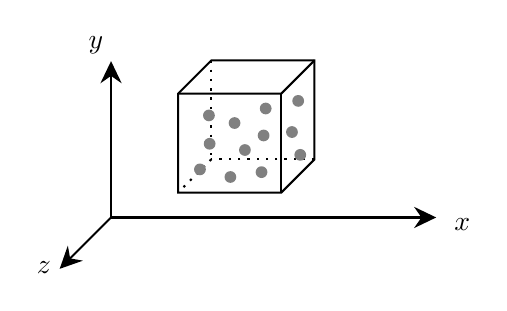
\begin{tikzpicture}[x=0.75pt,y=0.75pt,yscale=-1,xscale=1]
	%uncomment if require: \path (0,300); %set diagram left start at 0, and has height of 300

	%Straight Lines [id:da45879241397607173] 
	\draw  [dash pattern={on 0.84pt off 2.51pt}]  (217.33,94.33) -- (217.33,142) ;
	%Straight Lines [id:da9742441093997318] 
	\draw  [dash pattern={on 0.84pt off 2.51pt}]  (267,142) -- (217.13,142) ;
	%Straight Lines [id:da6927479790989322] 
	\draw  [dash pattern={on 0.84pt off 2.51pt}]  (217.33,142) -- (201.63,157.7) ;
	%Straight Lines [id:da4354392473018709] 
	\draw    (169,170) -- (169,97.67) ;
	\draw [shift={(169,94.67)}, rotate = 450] [fill={rgb, 255:red, 0; green, 0; blue, 0 }  ][line width=0.08]  [draw opacity=0] (10.72,-5.15) -- (0,0) -- (10.72,5.15) -- (7.12,0) -- cycle    ;
	%Straight Lines [id:da9740500633855294] 
	\draw    (169,170) -- (146.37,192.63) ;
	\draw [shift={(144.25,194.75)}, rotate = 315] [fill={rgb, 255:red, 0; green, 0; blue, 0 }  ][line width=0.08]  [draw opacity=0] (10.72,-5.15) -- (0,0) -- (10.72,5.15) -- (7.12,0) -- cycle    ;
	%Straight Lines [id:da17051109556175215] 
	\draw    (169,170) -- (322.67,170) ;
	\draw [shift={(325.67,170)}, rotate = 180] [fill={rgb, 255:red, 0; green, 0; blue, 0 }  ][line width=0.08]  [draw opacity=0] (10.72,-5.15) -- (0,0) -- (10.72,5.15) -- (7.12,0) -- cycle    ;
	%Shape: Cube [id:dp559325738726933] 
	\draw   (201.33,110.33) -- (217.33,94.33) -- (267,94.33) -- (267,142) -- (251,158) -- (201.33,158) -- cycle ; \draw   (267,94.33) -- (251,110.33) -- (201.33,110.33) ; \draw   (251,110.33) -- (251,158) ;
	%Shape: Circle [id:dp3295026946934616] 
	\draw  [draw opacity=0][fill={rgb, 255:red, 128; green, 128; blue, 128 }  ,fill opacity=1 ] (213.33,120.83) .. controls (213.33,119.27) and (214.6,118) .. (216.17,118) .. controls (217.73,118) and (219,119.27) .. (219,120.83) .. controls (219,122.4) and (217.73,123.67) .. (216.17,123.67) .. controls (214.6,123.67) and (213.33,122.4) .. (213.33,120.83) -- cycle ;
	%Shape: Circle [id:dp8704491879909637] 
	\draw  [draw opacity=0][fill={rgb, 255:red, 128; green, 128; blue, 128 }  ,fill opacity=1 ] (238.67,148.17) .. controls (238.67,146.6) and (239.94,145.33) .. (241.5,145.33) .. controls (243.06,145.33) and (244.33,146.6) .. (244.33,148.17) .. controls (244.33,149.73) and (243.06,151) .. (241.5,151) .. controls (239.94,151) and (238.67,149.73) .. (238.67,148.17) -- cycle ;
	%Shape: Circle [id:dp9279661658238063] 
	\draw  [draw opacity=0][fill={rgb, 255:red, 128; green, 128; blue, 128 }  ,fill opacity=1 ] (256.33,113.83) .. controls (256.33,112.27) and (257.6,111) .. (259.17,111) .. controls (260.73,111) and (262,112.27) .. (262,113.83) .. controls (262,115.4) and (260.73,116.67) .. (259.17,116.67) .. controls (257.6,116.67) and (256.33,115.4) .. (256.33,113.83) -- cycle ;
	%Shape: Circle [id:dp6636119609330704] 
	\draw  [draw opacity=0][fill={rgb, 255:red, 128; green, 128; blue, 128 }  ,fill opacity=1 ] (253.33,128.83) .. controls (253.33,127.27) and (254.6,126) .. (256.17,126) .. controls (257.73,126) and (259,127.27) .. (259,128.83) .. controls (259,130.4) and (257.73,131.67) .. (256.17,131.67) .. controls (254.6,131.67) and (253.33,130.4) .. (253.33,128.83) -- cycle ;
	%Shape: Circle [id:dp7894888587590783] 
	\draw  [draw opacity=0][fill={rgb, 255:red, 128; green, 128; blue, 128 }  ,fill opacity=1 ] (257.33,139.83) .. controls (257.33,138.27) and (258.6,137) .. (260.17,137) .. controls (261.73,137) and (263,138.27) .. (263,139.83) .. controls (263,141.4) and (261.73,142.67) .. (260.17,142.67) .. controls (258.6,142.67) and (257.33,141.4) .. (257.33,139.83) -- cycle ;
	%Shape: Circle [id:dp21747914903436993] 
	\draw  [draw opacity=0][fill={rgb, 255:red, 128; green, 128; blue, 128 }  ,fill opacity=1 ] (240.67,117.5) .. controls (240.67,115.94) and (241.94,114.67) .. (243.5,114.67) .. controls (245.06,114.67) and (246.33,115.94) .. (246.33,117.5) .. controls (246.33,119.06) and (245.06,120.33) .. (243.5,120.33) .. controls (241.94,120.33) and (240.67,119.06) .. (240.67,117.5) -- cycle ;
	%Shape: Circle [id:dp7272550201057293] 
	\draw  [draw opacity=0][fill={rgb, 255:red, 128; green, 128; blue, 128 }  ,fill opacity=1 ] (209,146.83) .. controls (209,145.27) and (210.27,144) .. (211.83,144) .. controls (213.4,144) and (214.67,145.27) .. (214.67,146.83) .. controls (214.67,148.4) and (213.4,149.67) .. (211.83,149.67) .. controls (210.27,149.67) and (209,148.4) .. (209,146.83) -- cycle ;
	%Shape: Circle [id:dp6688552083133636] 
	\draw  [draw opacity=0][fill={rgb, 255:red, 128; green, 128; blue, 128 }  ,fill opacity=1 ] (230.67,137.5) .. controls (230.67,135.94) and (231.94,134.67) .. (233.5,134.67) .. controls (235.06,134.67) and (236.33,135.94) .. (236.33,137.5) .. controls (236.33,139.06) and (235.06,140.33) .. (233.5,140.33) .. controls (231.94,140.33) and (230.67,139.06) .. (230.67,137.5) -- cycle ;
	%Shape: Circle [id:dp4611735824001546] 
	\draw  [draw opacity=0][fill={rgb, 255:red, 128; green, 128; blue, 128 }  ,fill opacity=1 ] (225.67,124.5) .. controls (225.67,122.94) and (226.94,121.67) .. (228.5,121.67) .. controls (230.06,121.67) and (231.33,122.94) .. (231.33,124.5) .. controls (231.33,126.06) and (230.06,127.33) .. (228.5,127.33) .. controls (226.94,127.33) and (225.67,126.06) .. (225.67,124.5) -- cycle ;
	%Shape: Circle [id:dp8099918451310808] 
	\draw  [draw opacity=0][fill={rgb, 255:red, 128; green, 128; blue, 128 }  ,fill opacity=1 ] (213.67,134.5) .. controls (213.67,132.94) and (214.94,131.67) .. (216.5,131.67) .. controls (218.06,131.67) and (219.33,132.94) .. (219.33,134.5) .. controls (219.33,136.06) and (218.06,137.33) .. (216.5,137.33) .. controls (214.94,137.33) and (213.67,136.06) .. (213.67,134.5) -- cycle ;
	%Shape: Circle [id:dp6693692291433728] 
	\draw  [draw opacity=0][fill={rgb, 255:red, 128; green, 128; blue, 128 }  ,fill opacity=1 ] (223.67,150.5) .. controls (223.67,148.94) and (224.94,147.67) .. (226.5,147.67) .. controls (228.06,147.67) and (229.33,148.94) .. (229.33,150.5) .. controls (229.33,152.06) and (228.06,153.33) .. (226.5,153.33) .. controls (224.94,153.33) and (223.67,152.06) .. (223.67,150.5) -- cycle ;
	%Shape: Circle [id:dp5611121559728784] 
	\draw  [draw opacity=0][fill={rgb, 255:red, 128; green, 128; blue, 128 }  ,fill opacity=1 ] (239.67,130.5) .. controls (239.67,128.94) and (240.94,127.67) .. (242.5,127.67) .. controls (244.06,127.67) and (245.33,128.94) .. (245.33,130.5) .. controls (245.33,132.06) and (244.06,133.33) .. (242.5,133.33) .. controls (240.94,133.33) and (239.67,132.06) .. (239.67,130.5) -- cycle ;

	% Text Node
	\draw (161.67,87.17) node    {$y$};
	% Text Node
	\draw (338.17,173.33) node    {$x$};
	% Text Node
	\draw (136.67,194.33) node    {$z$};

	\end{tikzpicture}
\end{figure}
\FloatBarrier
Come si vedrà più in dettaglio, la prima ipotesi implica che la velocità media vettoriale sia nulla. La terza che negli urti tra molecole si conservano quantità di moto ed energia, mentre nell'urto di una molecola contro una parete si conserva solo l'energia. Dalla quarta ipotesi deriva che l'energia potenziale interna è nulla e quindi la sola forma di energia è quella cinetica.
Sulla base del modello cinetico, è stata sviluppata, nella seconda metà dell'800, la \textbf{teoria cinetica dei gas}, che permette di arrivare a previsioni sul comportamento dei gas, verificabili sperimentalmente.

\subsection{La visione microscopica della pressione}

Si ha un contenitore cubico con $n$ molecole che si muovono caoticamente e ogni molecola $i$-esima possiede la velocità vettoriale $\vec{v}_i$. Se si vuole calcolare il valore medio della velocità vettoriale di tutte le particelle si trova che esso è pari a $0$ perché il moto è caotico. Se $n$ particelle vanno a sinistra ce ne saranno altrettante che vanno a destra. Le forze esterne sono trascurabili e quindi il centro di massa ha velocità costante, in particolare pari a $0$. La particella $i$-esima avrà una componente lungo $x,y$ e $z$. L'obbiettivo che ci si pone è di legare la pressione al moto microscopico delle particelle. Si parte dalla pressione che si sente sulla parete $yz$ del recipiente. Essa sarà dovuta agli urti delle particelle contro la parete, sarà la forza totale esercitata dalle molecole, divisa per l'area della parete. La pressione è frutto soltanto delle forze ortogonali alla superficie, quindi conta soltanto la forza che sta agendo in direzione $x$. La forza totale è la somma estesa a tutte le molecole della forza generata dalla singola molecola in direzione $x$.

\[
	p = \frac{\norm{\vec{F}_{tot,x}} }{a^2} = \frac{\sum_{i=1}^N F_{x,i}}{a^2}
\]

Per comodità si trasforma il disegno da tridimensionale a bidimensionale, si ha la parete su cui vanno a urtare le varie molecole. Si consideri la molecola $i$-esima che sta arrivando con velocità qualunque.

\begin{figure}[htpb]
	\centering

	\tikzset{every picture/.style={line width=0.75pt}} %set default line width to 0.75pt        

	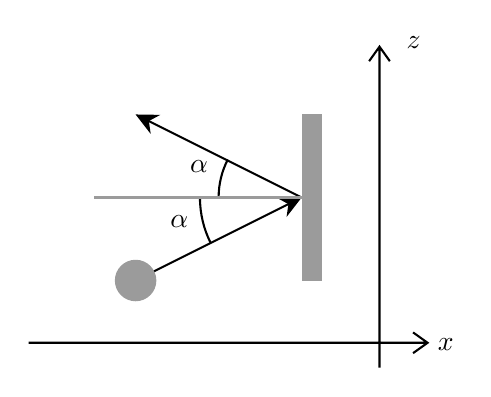
\begin{tikzpicture}[x=0.75pt,y=0.75pt,yscale=-1,xscale=1]
	%uncomment if require: \path (0,300); %set diagram left start at 0, and has height of 300

	%Shape: Axis 2D [id:dp18325872511828445] 
	\draw  (68.5,190) -- (260.67,190)(237.5,47.33) -- (237.5,202) (253.67,185) -- (260.67,190) -- (253.67,195) (232.5,54.33) -- (237.5,47.33) -- (242.5,54.33)  ;
	%Straight Lines [id:da46888513249136965] 
	\draw    (120,160) -- (197.32,121.34) ;
	\draw [shift={(200,120)}, rotate = 513.4300000000001] [fill={rgb, 255:red, 0; green, 0; blue, 0 }  ][line width=0.08]  [draw opacity=0] (10.72,-5.15) -- (0,0) -- (10.72,5.15) -- (7.12,0) -- cycle    ;
	%Straight Lines [id:da752842138682754] 
	\draw    (122.68,81.34) -- (200,120) ;
	\draw [shift={(120,80)}, rotate = 26.57] [fill={rgb, 255:red, 0; green, 0; blue, 0 }  ][line width=0.08]  [draw opacity=0] (10.72,-5.15) -- (0,0) -- (10.72,5.15) -- (7.12,0) -- cycle    ;
	%Shape: Rectangle [id:dp8263956807721704] 
	\draw  [draw opacity=0][fill={rgb, 255:red, 155; green, 155; blue, 155 }  ,fill opacity=1 ] (210,80) -- (200,80) -- (200,160) -- (210,160) -- cycle ;
	%Shape: Arc [id:dp42415565235130726] 
	\draw  [draw opacity=0] (160,120.49) .. controls (160,120.33) and (160,120.16) .. (160,120) .. controls (160,113.42) and (161.59,107.22) .. (164.4,101.74) -- (200,120) -- cycle ; \draw   (160,120.49) .. controls (160,120.33) and (160,120.16) .. (160,120) .. controls (160,113.42) and (161.59,107.22) .. (164.4,101.74) ;
	%Shape: Circle [id:dp9782826031645953] 
	\draw  [draw opacity=0][fill={rgb, 255:red, 155; green, 155; blue, 155 }  ,fill opacity=1 ] (110,160) .. controls (110,154.48) and (114.48,150) .. (120,150) .. controls (125.52,150) and (130,154.48) .. (130,160) .. controls (130,165.52) and (125.52,170) .. (120,170) .. controls (114.48,170) and (110,165.52) .. (110,160) -- cycle ;
	%Shape: Arc [id:dp33191213110278794] 
	\draw  [draw opacity=0] (156.04,141.66) .. controls (152.83,135.16) and (151.02,127.85) .. (151,120.11) -- (200,120) -- cycle ; \draw   (156.04,141.66) .. controls (152.83,135.16) and (151.02,127.85) .. (151,120.11) ;
	%Straight Lines [id:da6672059317477186] 
	\draw [color={rgb, 255:red, 155; green, 155; blue, 155 }  ,draw opacity=1 ]   (100,120) -- (200,120) ;

	% Text Node
	\draw (254,45.5) node    {$z$};
	% Text Node
	\draw (269.5,191) node    {$x$};
	% Text Node
	\draw (150.5,105) node    {$\alpha $};
	% Text Node
	\draw (141,131.5) node    {$\alpha $};

	\end{tikzpicture}
\end{figure}
\FloatBarrier
Gli urti sono elastici. Quindi la velocità dopo l'urto sarà la stessa perché l'energia cinetica si conserva. Visto che non c'è alcuna forza di attrito, la componente della velocità in direzione parallela alla parete non cambierà. Ciò significa che l'unica cosa che succede è che la componente $v_{i,x}$ semplicemente si ribalta e diventa $-v_{i,x}$. Quindi l'unica componente della velocità che varia è quella in $x$. Quando una particella urta una parete in modo perfettamente elastico, l'urto è speculare. Rispetto alla normale i due angoli sono uguali. La quantità di moto in direzione $x$ della particella è cambiata perché si è ribaltata di segno. Ciò è accaduto perché ha ricevuto una forza impulsiva $\vec{F}_{i,x}$ dalla parete. Si va a calcolarla. La variazione della quantità di moto in un urto è pari all'impulso della forza $\vec{F}_{i,x}$.

\[
	\Delta p = \int F_{x,i} dt = F_{x,i}\Delta t
\]

Ora il problema rimane il calcolo di $\vec{F}_{i,x}$, ossia la forza generata dalla particella $i$-esima sulla parete. Si ragioni sull'evoluzione temporale di quello che accade a questa parete a causa del fatto che la particella va a sbattere.
Si va a dare un grafico dell'andamento nel tempo della forza esercitata dalla parete sulla particella $i$-esima considerata.

\begin{figure}[htpb]
	\centering

	\tikzset{every picture/.style={line width=0.75pt}} %set default line width to 0.75pt        

	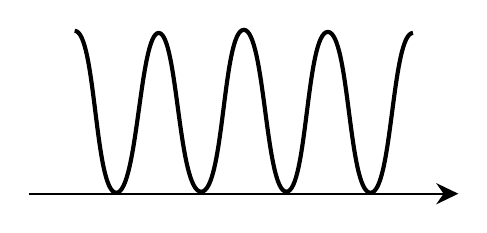
\begin{tikzpicture}[x=0.75pt,y=0.75pt,yscale=-1,xscale=1]
	%uncomment if require: \path (0,300); %set diagram left start at 0, and has height of 300

	% Plotting does not support converting to Tikz
	%Straight Lines [id:da5012780936511261] 
	\draw    (82.36,182.71) -- (286.36,182.71) ;
	\draw [shift={(289.36,182.71)}, rotate = 180] [fill={rgb, 255:red, 0; green, 0; blue, 0 }  ][line width=0.08]  [draw opacity=0] (10.72,-5.15) -- (0,0) -- (10.72,5.15) -- (7.12,0) -- cycle    ;
	%Curve Lines [id:da31123642176672517] 
	\draw [line width=1.5]    (104.5,104.25) .. controls (114.71,104) and (114.14,182) .. (124.5,182.25) .. controls (134.86,182.5) and (135.86,105.14) .. (145,105.25) .. controls (154.14,105.36) and (154.43,182) .. (165.5,181.75) .. controls (176.57,181.5) and (175.86,103.71) .. (186,103.75) .. controls (196.14,103.79) and (196.43,181.71) .. (206.5,181.75) .. controls (216.57,181.79) and (216.14,104.57) .. (226.5,104.75) .. controls (236.86,104.93) and (236.43,182) .. (247,182.25) .. controls (257.57,182.5) and (257.29,105.14) .. (267.5,105.25) ;

	\end{tikzpicture}
\end{figure}
\FloatBarrier
La particella rimbalza indietro e si mette a muoversi nell'altra direzione. Dopo un certo intervallo di tempo va a risbattere contro una stessa parete. Quindi essa urta le pareti continuamente. C'è un continuo di forze impulsive esercitate dalla particella su quella parete di intensità $\vec{F}_{i,x}$. Per valutare l'intervallo di tempo che intercorre fra un urto e il successivo, conta il tempo medio che ci mette la particella a fare avanti e indietro e quindi conta spazio / velocità. Lo spazio è $2a$, la velocità della particella è quella nella direzione $x$.

\[
	\Delta t = \frac{2a}{v_x }
\]

Nella realtà la particella è inclinata, ma la componente in $y$ non ha alcun effetto sul moto nella direzione considerata. Nella realtà inoltre essa muovendosi non continua a fare avanti indietro. Andrà a sbattere contro un'altra particella che si mette a muoversi. Per tenere conto di ciò si sfrutta il fatto che gli urti sono elastici. Quando un corpo urta in maniera elastica un corpo inizialmente fermo, il primo che era in moto si ferma e trasferisce tutta la sua quantità di moto al secondo. La particella urta una seconda particella, la prima si ferma e va avanti la seconda. Questo fa sì che il moto delle particelle possa essere pensato come quello di un'unica particella che si muove. Quello in figura è l'andamento nel tempo della forza, lo si vuole integrare nel tempo. Il numero di urti al secondo, ossia la frequenza degli urti, è l'inverso di $\Delta t$. Se tra un urto e l'altro passano $100 ms$, in un secondo ci sono 10 urti. Si può prendere il valore medio della forza fra un urto e il successivo e moltiplicarlo per l'intervallo di tempo per ottenere la variazione della quantità di moto in un intervallo di tempo. La relazione permette di calcolare quanto vale $\vec{F}_{i,x}$, quindi la forza che la particella $i$-esima imprime alla parete. $\vec{F}_{i,x}$ sarà quindi la variazione della quantità di moto in un urto fratto l'intervallo di tempo che intercorre fra un urto e il successivo.
Visto che che $\Delta p = 2m\,v_{x,i}$:

\[
	F_{x,i} = \frac{\Delta p_{\text{urto} } }{\Delta t} = \frac{2m\,v_{x,i} }{2a/v_{x,i} } = \frac{m\,v_{x,i}^2}{a} \qquad \text{impulso comunicato in un secondo}
\]

A questo punto si può sostituire il risultato nell'espressione della pressione vista come rapporto fra la forza esercitata da tutte le particelle sulla parere e l'area della parete stessa.

\[
	p = \frac{F_{tot,x}}{a^2} = \frac{\sum_{i=1}^N F_{i,x}  }{a^2} = \frac{\sum_{i=1}^N v_{x,i}^2\cdot m}{\underbrace{a^3}_V}
\]

La pressione dipende dal volume del recipiente e dal quadrato della velocità lungo $x$. Si attua un ultimo passaggio. Visto che la velocità vettoriale media non porta alcuna informazione, bisogna considerare un altro valore medio che dica quanto rapidamente si muovono le particelle. Si calcola il valore medio del quadrato della velocità, detto appunto velocità quadratica media.

\[
	\langle v^2 \rangle = \frac{1}{N} \sum_{i=1}^N (v_{x,i}^2 +v_{y,i}^2 + v_{z,i}^2)
\]

Esso si può esprimere anche in termini delle tre componenti.

\[
	\langle \vec{v} \rangle = 0 \qquad \langle v^2 \rangle = \langle v_x^2 +v_y^2 +v_z^2 \rangle = \langle v_x^2 \rangle + \langle v_y^2 \rangle + \langle v_z^2 \rangle
\]

Il valore medio di tre addendi si può anche scrivere come la somma dei valori medi degli addendi. Visto che le particelle sono tutte uguali e si muovono caoticamente in tutte le direzioni, ci si deve aspettare che, considerato il quadrato delle componenti, questi tre valori medi siano uguali. In media tutte le particelle si muovono rapide ugualmente in tutte tre le direzione. Allora questo valore medio al quadrato si può riscrivere come tre volte il valore medio della velocità quadratica media.

\[
	\langle v^2 \rangle = 3 \langle v_x^2 \rangle = 3 \frac{\sum_{i=1}^N v_{x,i}^2}{N} = \frac{3}{N} \sum_{i=1}^N v_{x,i}^2
\]

Andando a sostituirla nell'espressione per la pressione trovata in precedenza:

\[
	\boxed{p = \frac{mN\langle v^2 \rangle}{3V}}
\]

Si è arrivati a dire che la pressione che si va a misurare con un sensore sulla parete è fondamentalmente legata alla velocità quadratica media con cui si muovono le particelle e a quante sono. Più le particelle si muovono con velocità quadratica media elevata, più la pressione è elevata. Questa è la visione microscopica della pressione. Volendo là si può legare invece che alla velocità quadratica media, all'\textbf{energia cinetica media} delle molecole. Si definisce energia cinetica media di una molecola del gas, la quantità: $E_K = \frac{1}{2} m\langle v^2 \rangle$. Questa relazione si può riscrivere in modo tale che la pressione diventi:

\[
	\boxed{p = \frac{2}{3} \frac{N}{V} \langle E_K \rangle}
\]

\subsection{La visione microscopica della temperatura}

È noto che il prodotto pressione e volume è proporzionale a una certa quantità. Ci si aggiunge il risultato dato dell'equazione di stato dei gas perfetti. Il tutto perché si vuole avere una visione microscopica della temperatura.
Si ottiene che $pV = \frac{2}{3} N \langle E_K \rangle = nRT$. Attuando la sostituzione: $n=N/N_A$, si ha:

\[
	\frac{N}{N_A } RT = \frac{2}{3} N \langle E_K \rangle
\]

e il rapporto

\[
	\frac{R}{N_A } = k_B = \frac{8.314}{6.022 \times 10^{23} } = 1.3807 \times 10^{-23}\,J/K
\]
$R/N_A$ prende il nome di \emph{costante di Boltzmann}. Si ottiene che l'energia cinetica media delle particelle è:

\[
	k_B T = \frac{2}{3} \langle E_K \rangle \implies \boxed{\langle E_K \rangle = \frac{3}{2} k_B T}
\]

Questa è l'interpretazione microscopica della temperatura, o se si vuole, del moto delle particelle. Più un gas è caldo in temperatura, più le particelle si muovono con energia cinetica media elevata. L'agitazione termica è data dalla temperatura.

\emph{L'energia cinetica media traslazionale di una molecola di un gas ideale è proporzionale alla temperatura di un gas}.
